\section*{Appendix to chapter \ref{chap:routing}}

%figure : 3 time series (3 reservoirs) on average over the IP for both routings
\begin{figure}[htbp]
    \centering
    \begin{subfigure}[b]{0.48\textwidth}
        \caption{Groundwater reservoir average}
        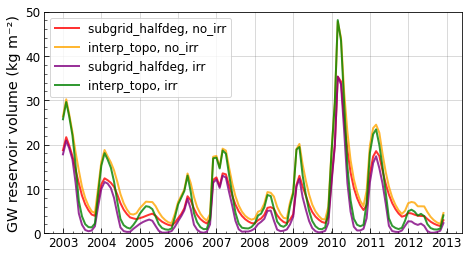
\includegraphics[width=\textwidth]{images/chap3/time_series/slowr_time_series.png}
    \end{subfigure}
        \begin{subfigure}[b]{0.48\textwidth}
        \caption{Groundwater reservoir average seasonal cycle}
        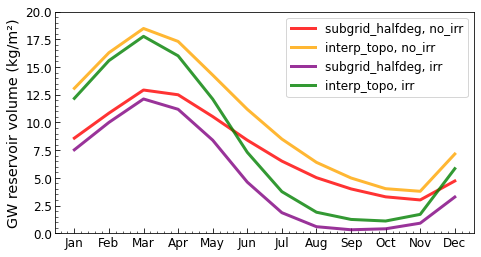
\includegraphics[width=\textwidth]{images/chap3/time_series/slowr_seasonal_cycle.png}
    \end{subfigure} \\
    
    \begin{subfigure}[b]{0.48\textwidth}
        \caption{Overland reservoir average}
        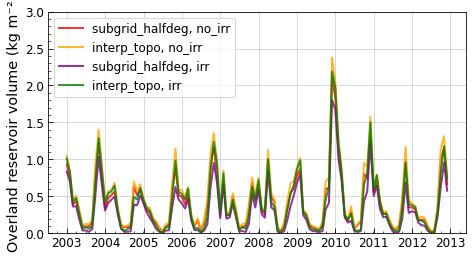
\includegraphics[width=\textwidth]{images/chap3/time_series/fastr_time_series.png}
    \end{subfigure}
    \begin{subfigure}[b]{0.48\textwidth}
        \caption{Overland reservoir average seasonal cycle}
        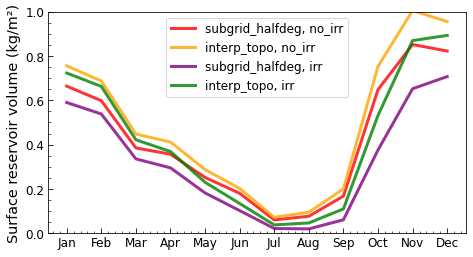
\includegraphics[width=\textwidth]{images/chap3/time_series/fastr_seasonal_cycle.png}
    \end{subfigure} \\
    
    \begin{subfigure}[b]{0.48\textwidth}
        \caption{River reservoir average}
        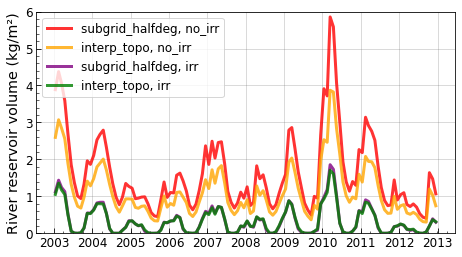
\includegraphics[width=\textwidth]{images/chap3/time_series/streamr_time_series.png}
    \end{subfigure} 
    \begin{subfigure}[b]{0.48\textwidth}
        \caption{River reservoir average seasonal cycle}
        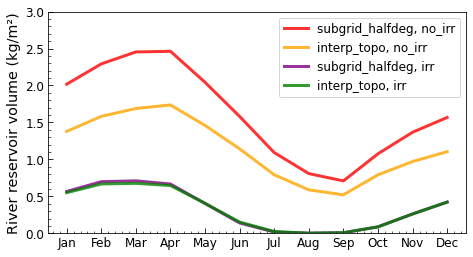
\includegraphics[width=\textwidth]{images/chap3/time_series/streamr_seasonal_cycle.png}
    \end{subfigure} \\

    \caption{Time series and seasonal cycles of reservoir volumes on average over the Iberian Peninsula domain.}
    \label{fig:reservoir_time_series}
\end{figure}

%figure : maps of diff vs ERA for 2 forcing sampling freqs
\begin{figure}[!h]
    \centering
    \begin{tabular}{cc}
        %total cc
        \begin{subfigure}[b]{0.33\textwidth}
            \caption{Total cloud cover bias\\(\%, \forcingoneh)}
            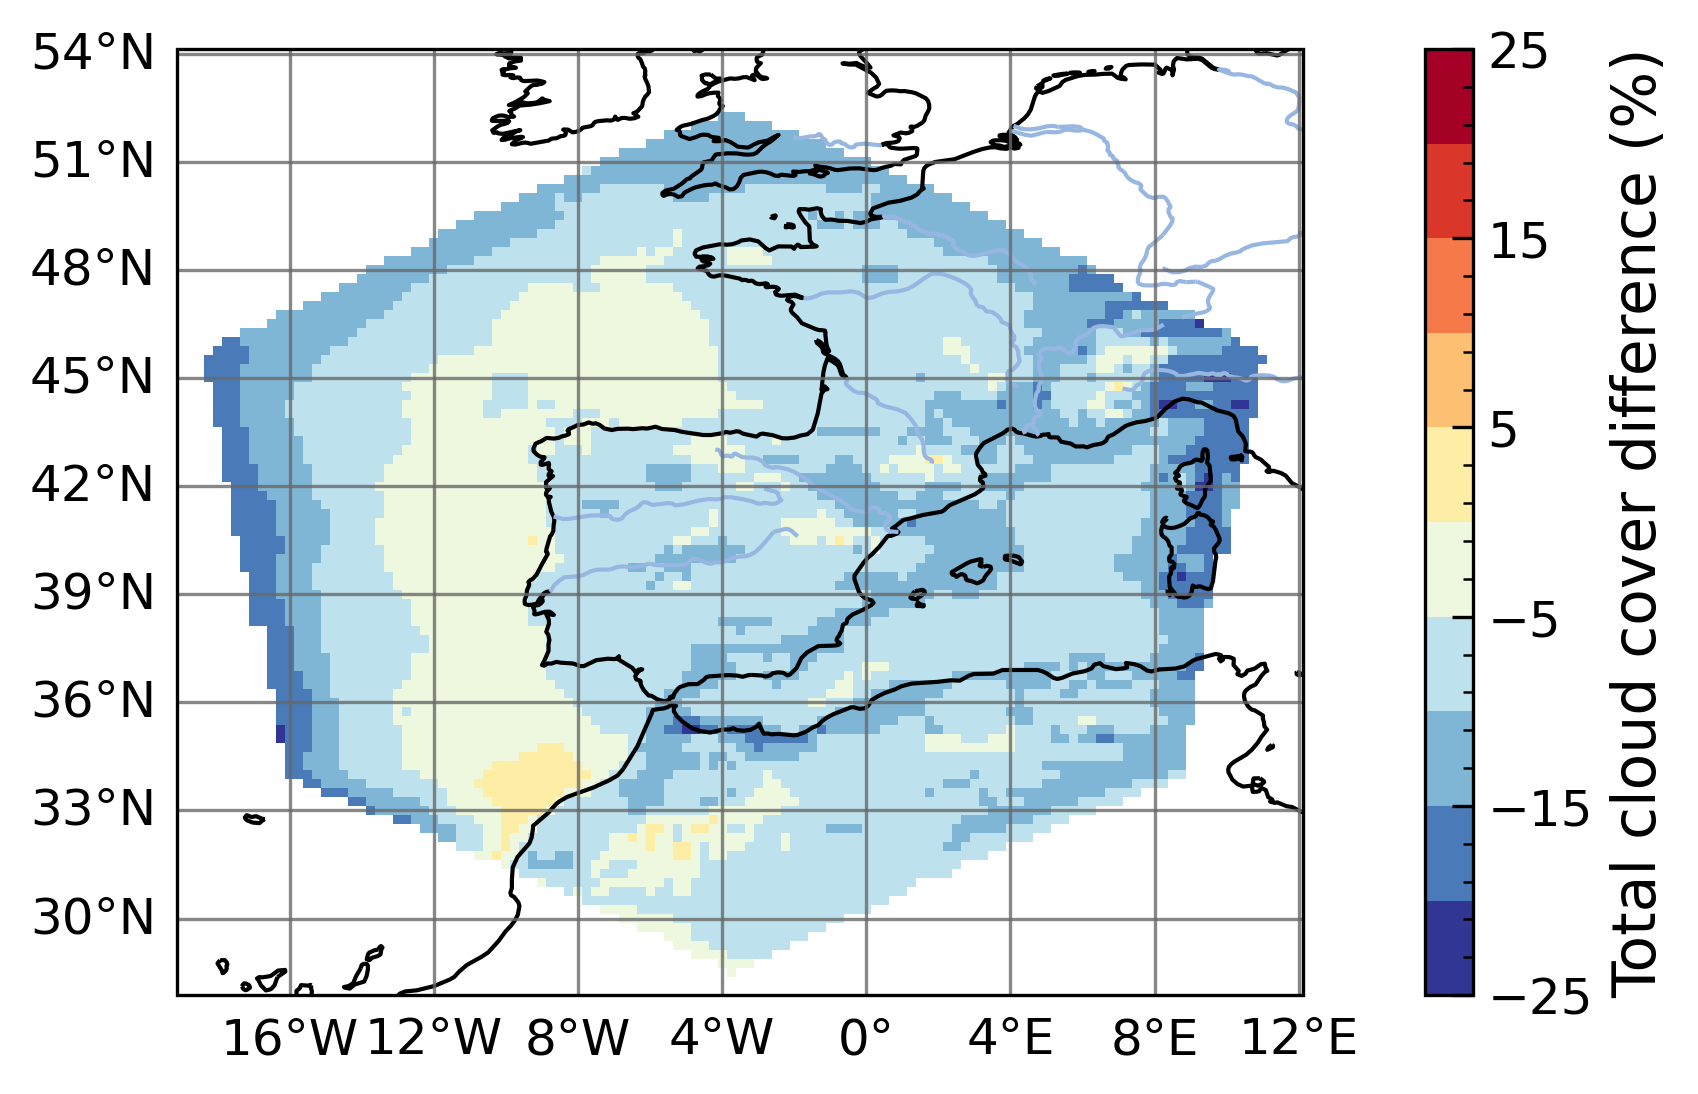
\includegraphics[width=\textwidth]{images/chap4/forcing_sampling_freq/diff_map_cldt_lmdz1h_era.png}
        \end{subfigure} &
        \begin{subfigure}[b]{0.33\textwidth}
            \caption{Total cloud cover bias\\(\%, \forcingsixh)}
            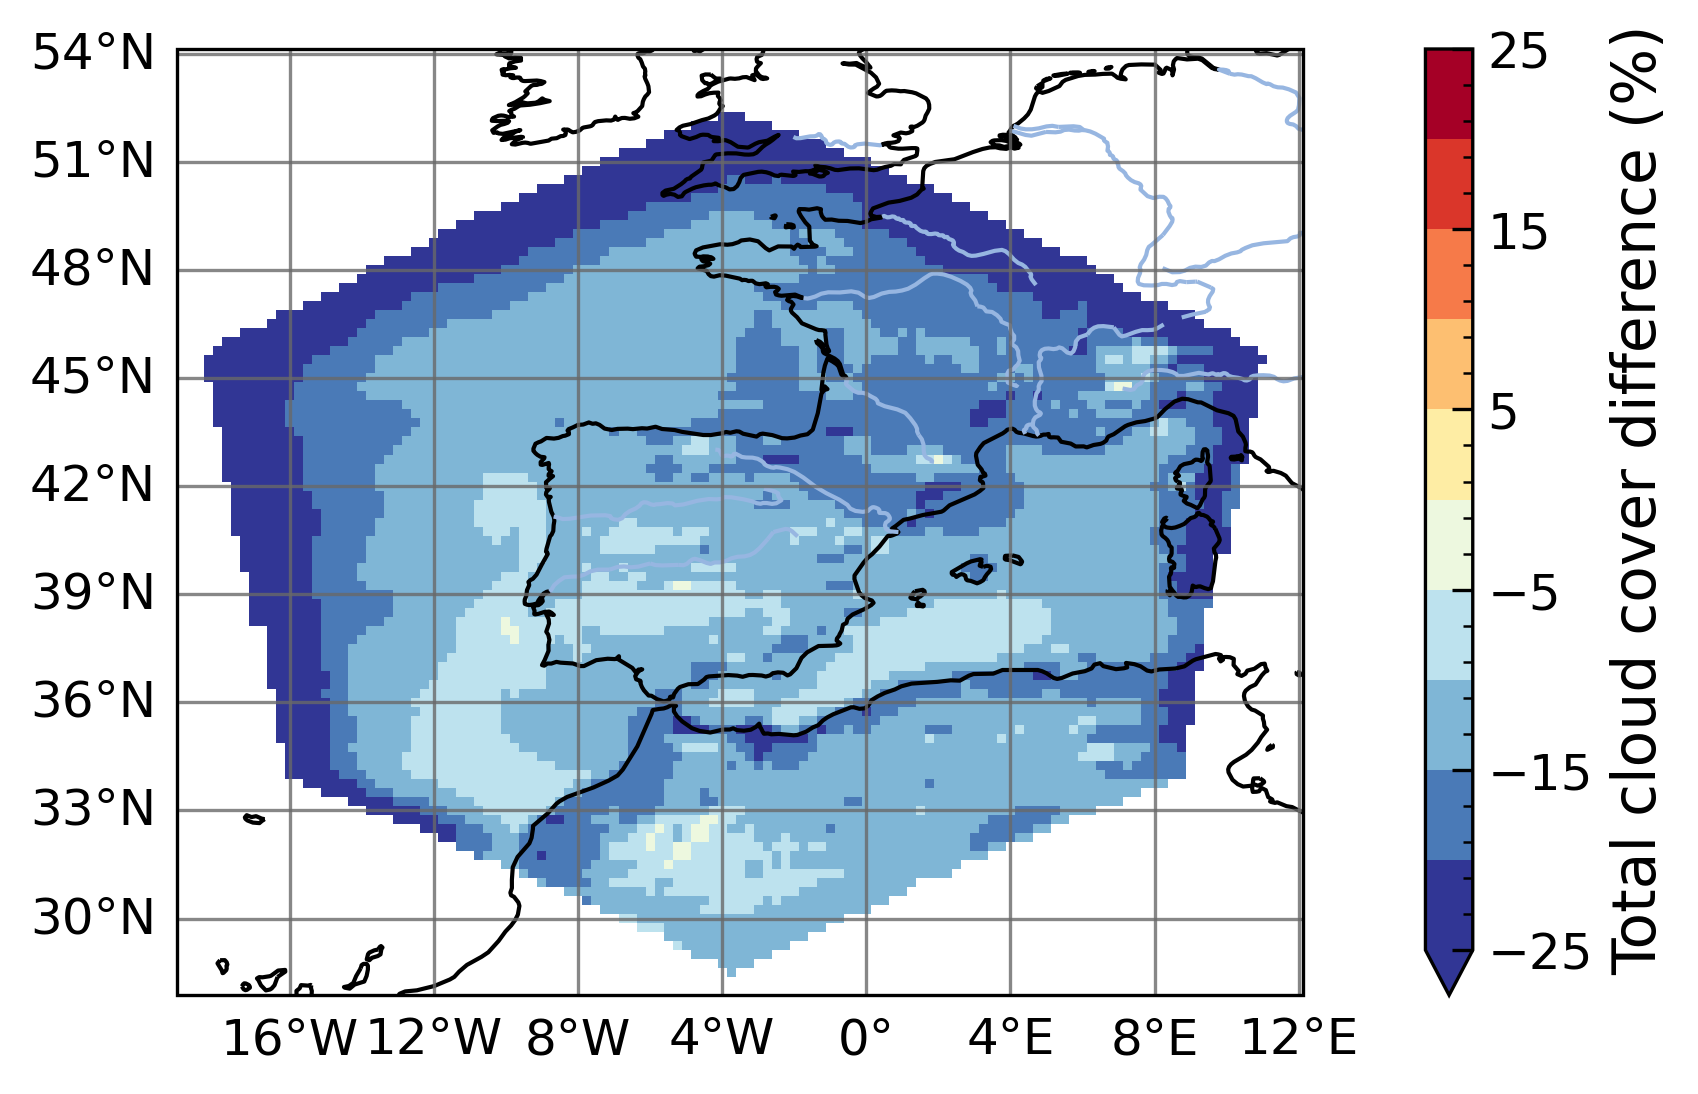
\includegraphics[width=\textwidth]{images/chap4/forcing_sampling_freq/diff_map_cldt_lmdz6h_era.png}
        \end{subfigure}\\
        %low cc
        \begin{subfigure}[b]{0.33\textwidth}
            \caption{Low cloud cover bias\\(\%, \forcingoneh)}
            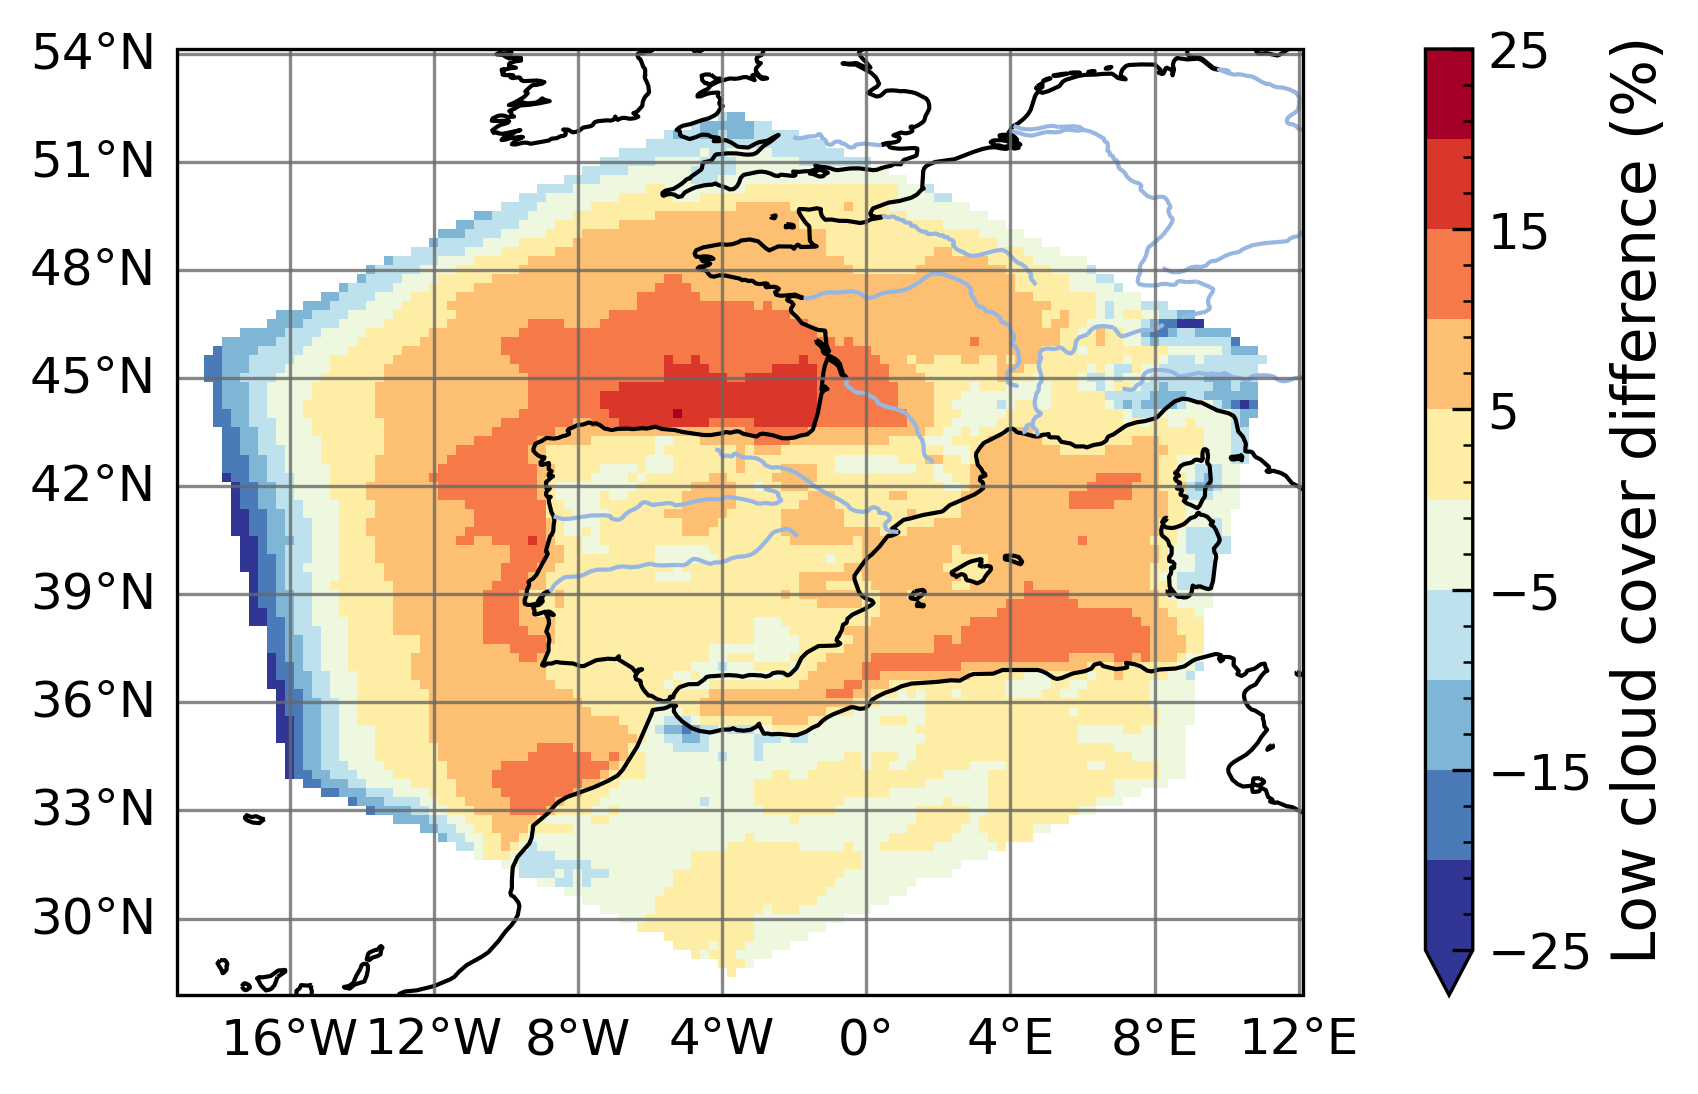
\includegraphics[width=\textwidth]{images/chap4/forcing_sampling_freq/diff_map_cldl_lmdz1h_era.png}
        \end{subfigure} &
        \begin{subfigure}[b]{0.33\textwidth}
            \caption{Low cloud cover bias\\(\%, \forcingsixh)}
            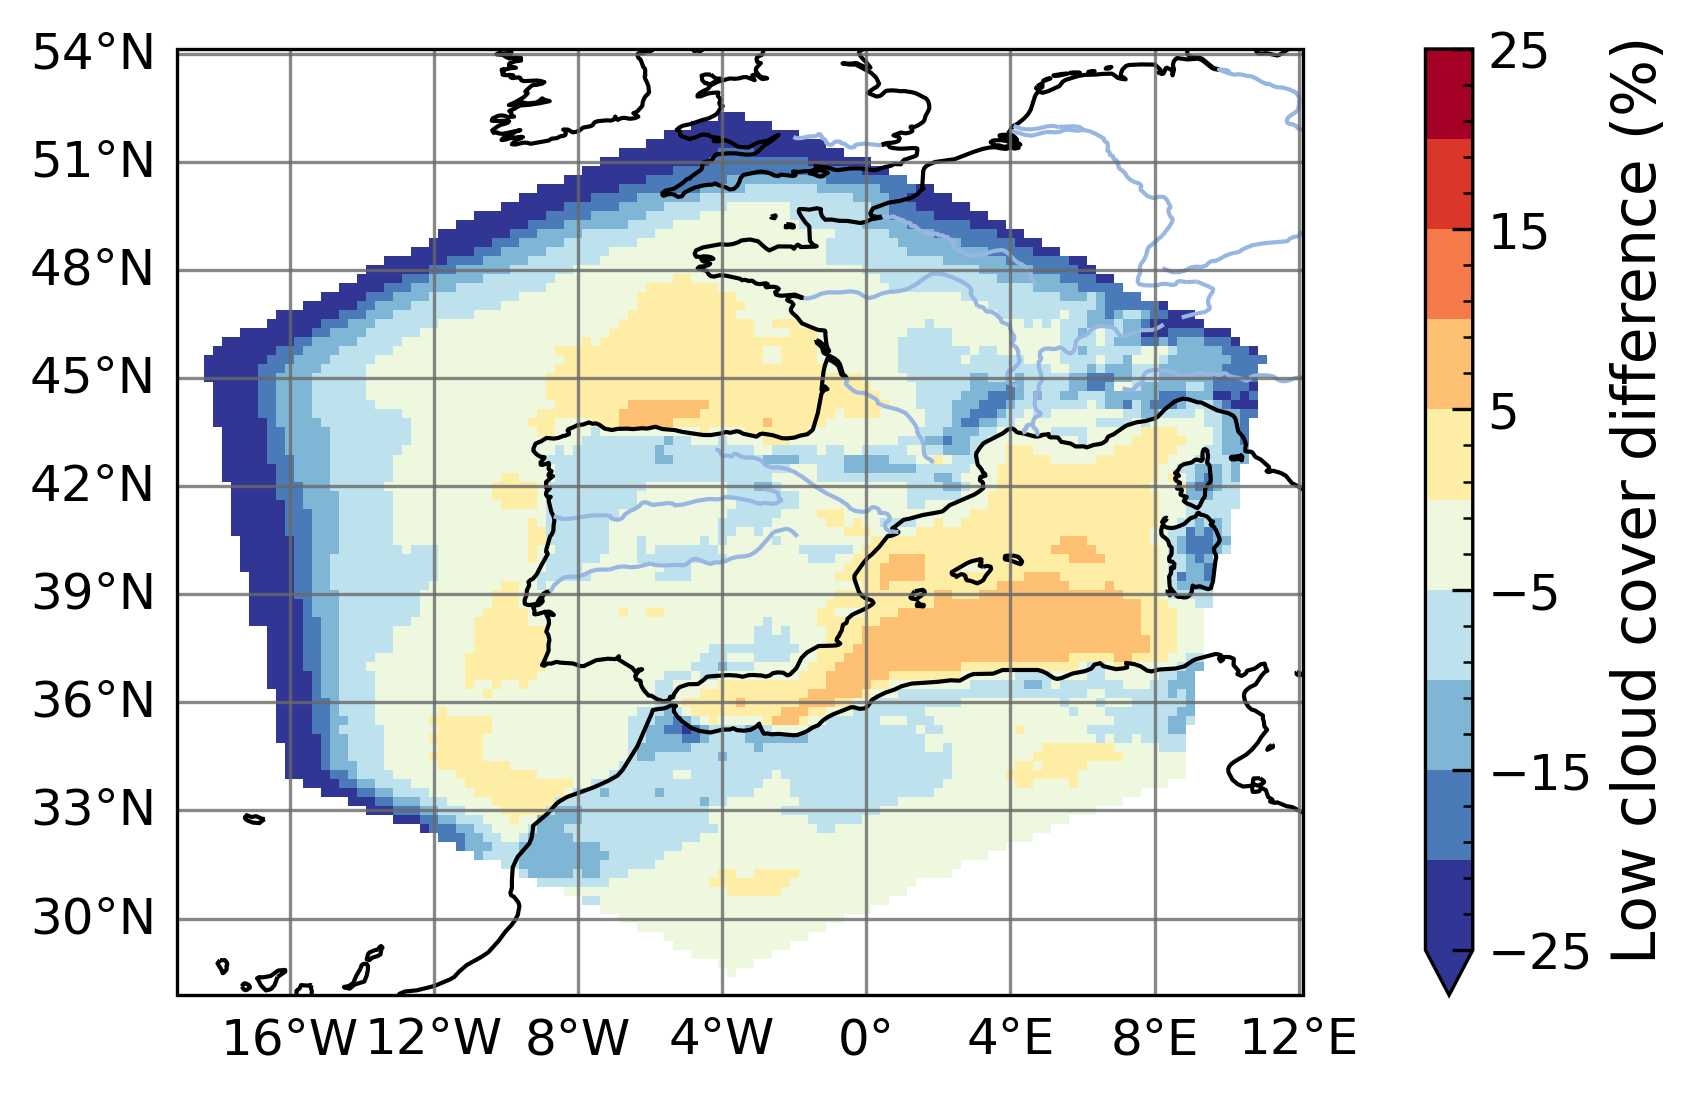
\includegraphics[width=\textwidth]{images/chap4/forcing_sampling_freq/diff_map_cldl_lmdz6h_era.png}
        \end{subfigure}
    \end{tabular}
    \caption{Biases of cloud cover for the simulations with hourly and 6-hourly forcing data, compared to ERA (2013).}
    \label{fig:forcing_sampling_freq_ERA_diff_maps_appendix}
\end{figure}

\clearpage

\section*{Appendix to chapter \ref{chap:forcing}}
%Forcing influence

%figure : maps of relative diff vs ERA for 3 domain sizes
%todo:captions
\begin{figure}[htbp]
    \centering
    \begin{tabular}{ccc}
        %precip
        \begin{subfigure}[b]{0.33\textwidth}
            \caption{}
            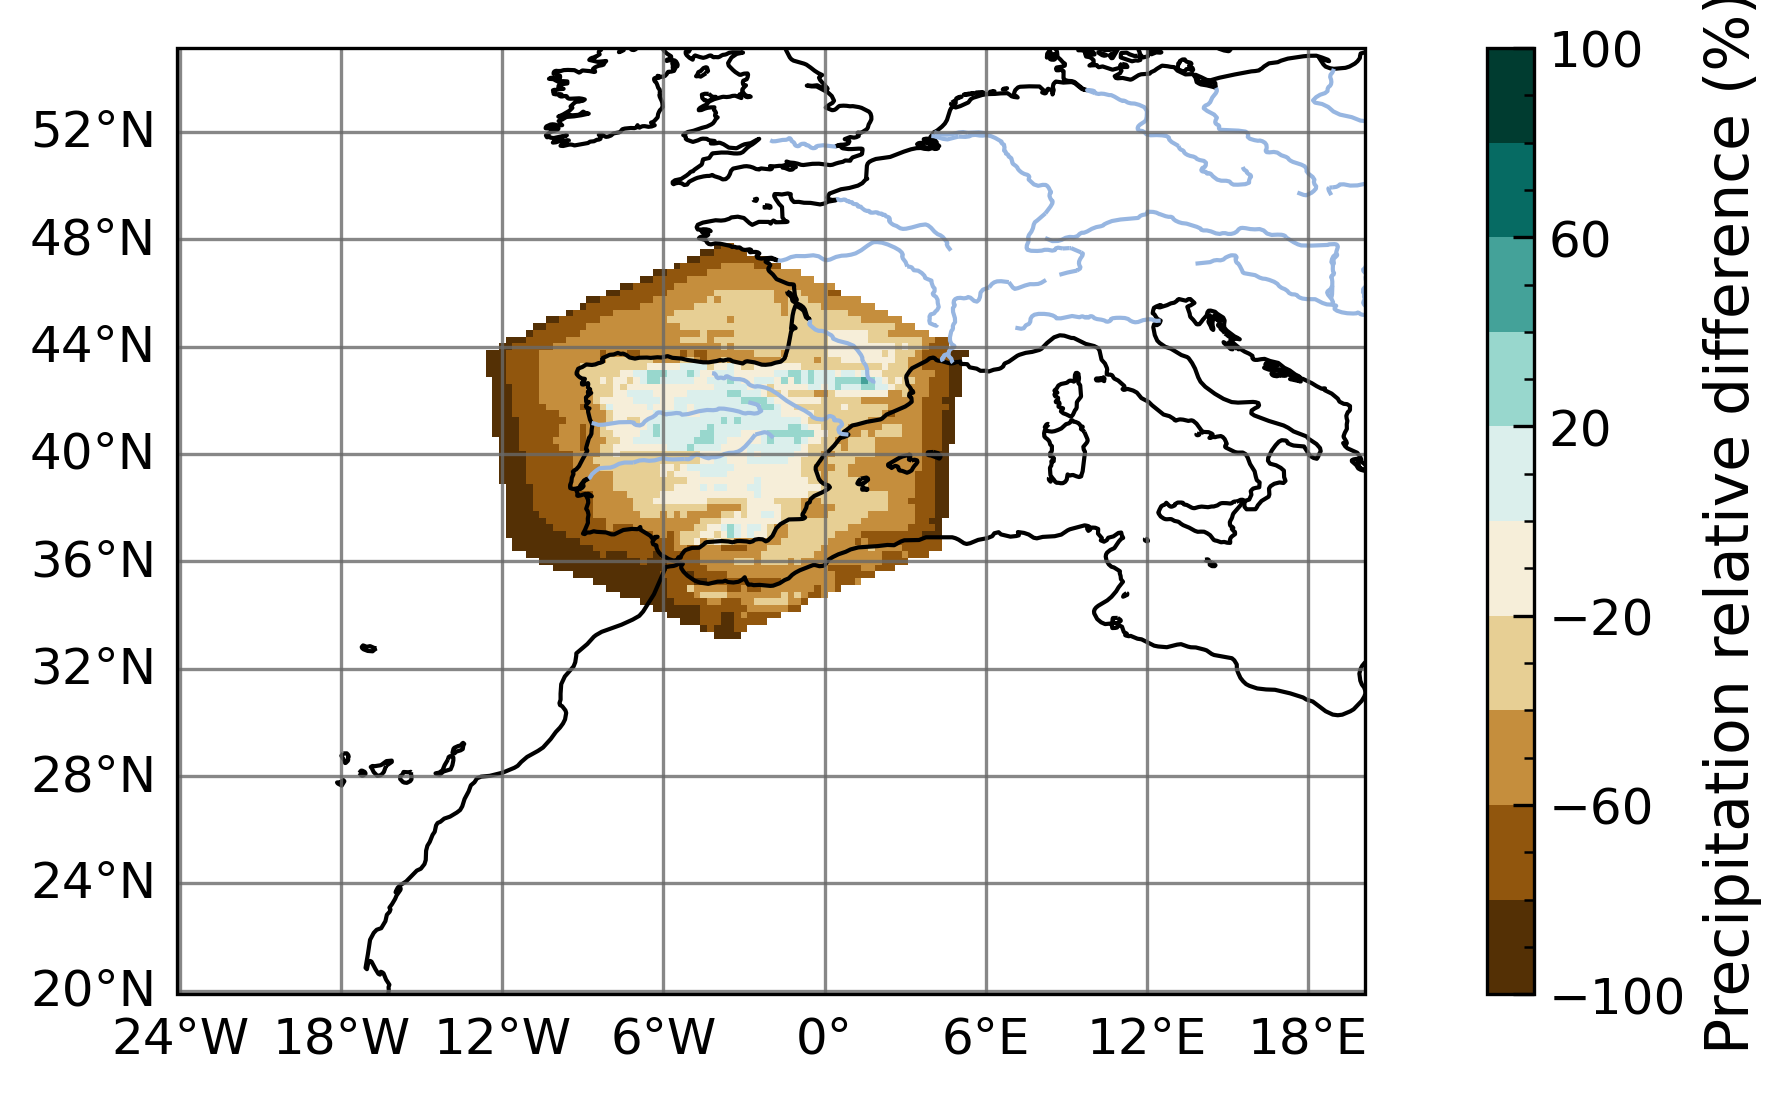
\includegraphics[width=\textwidth]{images/chap4/domain_size/rel_diff_map_precip_era_LAM_1000km_NBP40.png}
        \end{subfigure} &
        \begin{subfigure}[b]{0.33\textwidth}
            \caption{}
            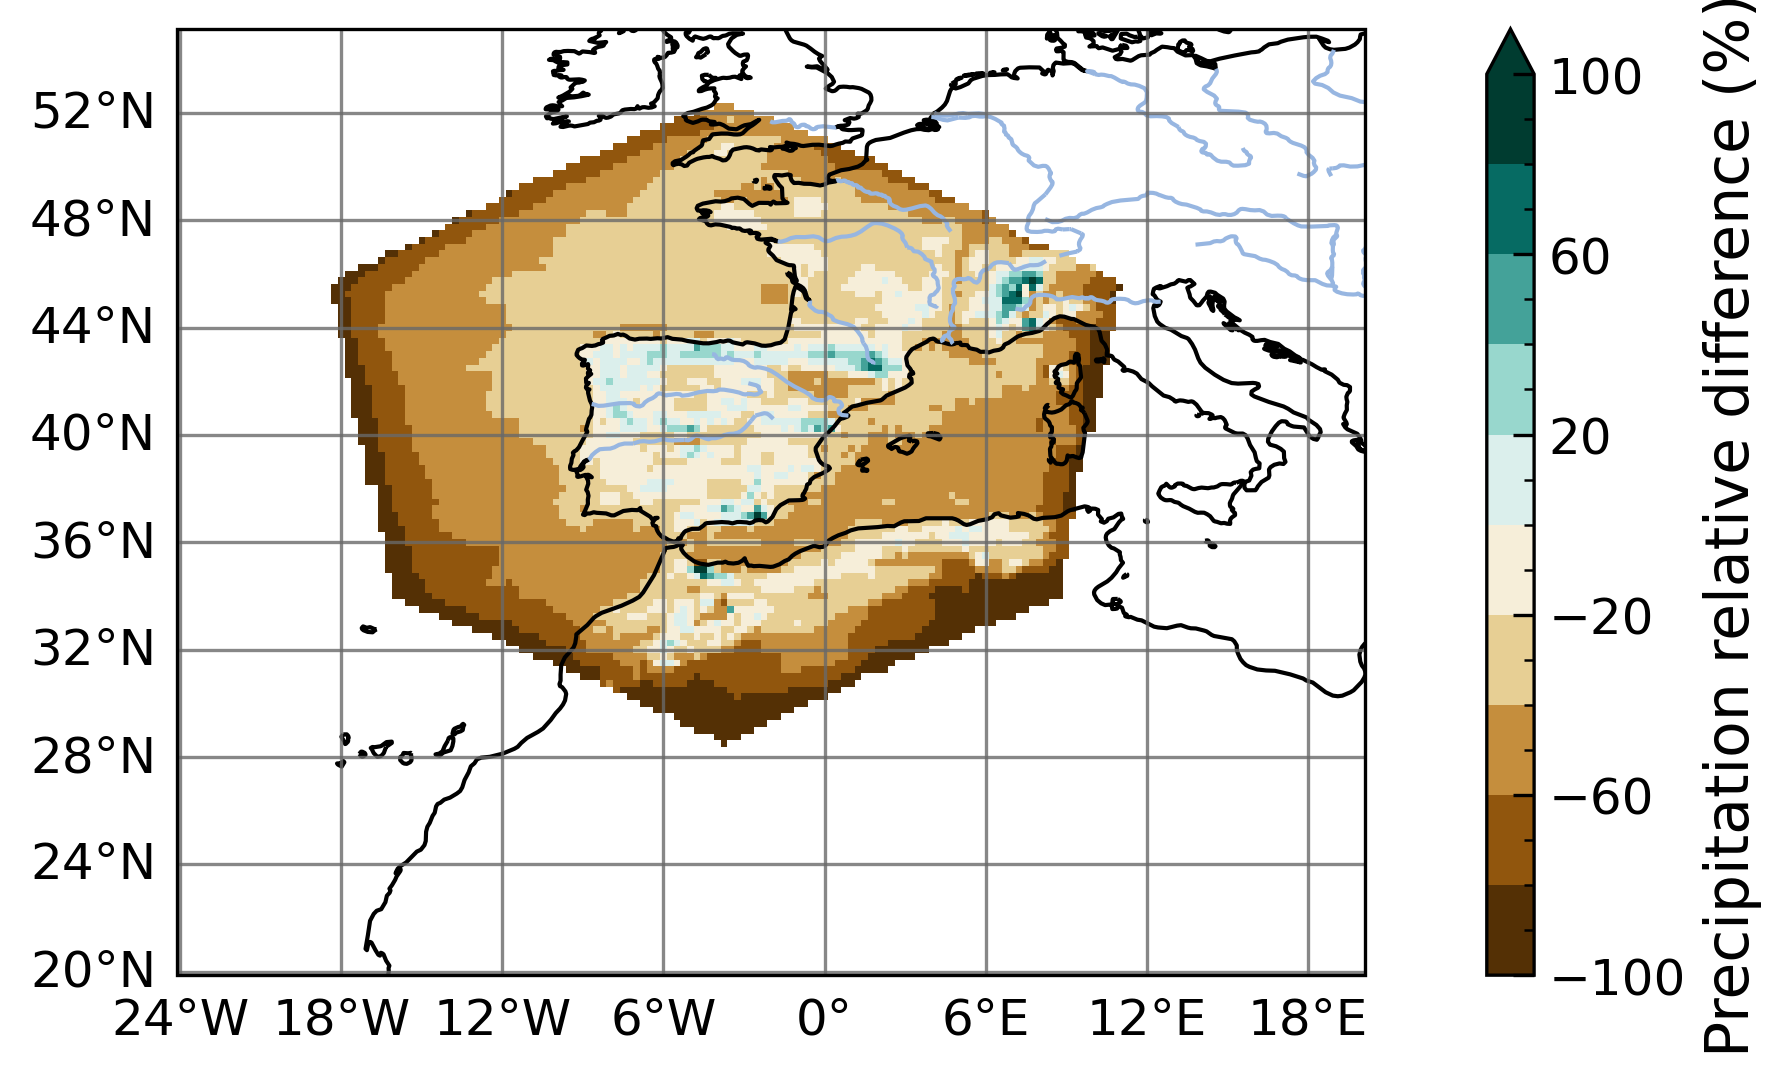
\includegraphics[width=\textwidth]{images/chap4/domain_size/rel_diff_map_precip_era_LAM_1500km_NBP60.png}
        \end{subfigure} &
        \begin{subfigure}[b]{0.33\textwidth}
            \caption{}
            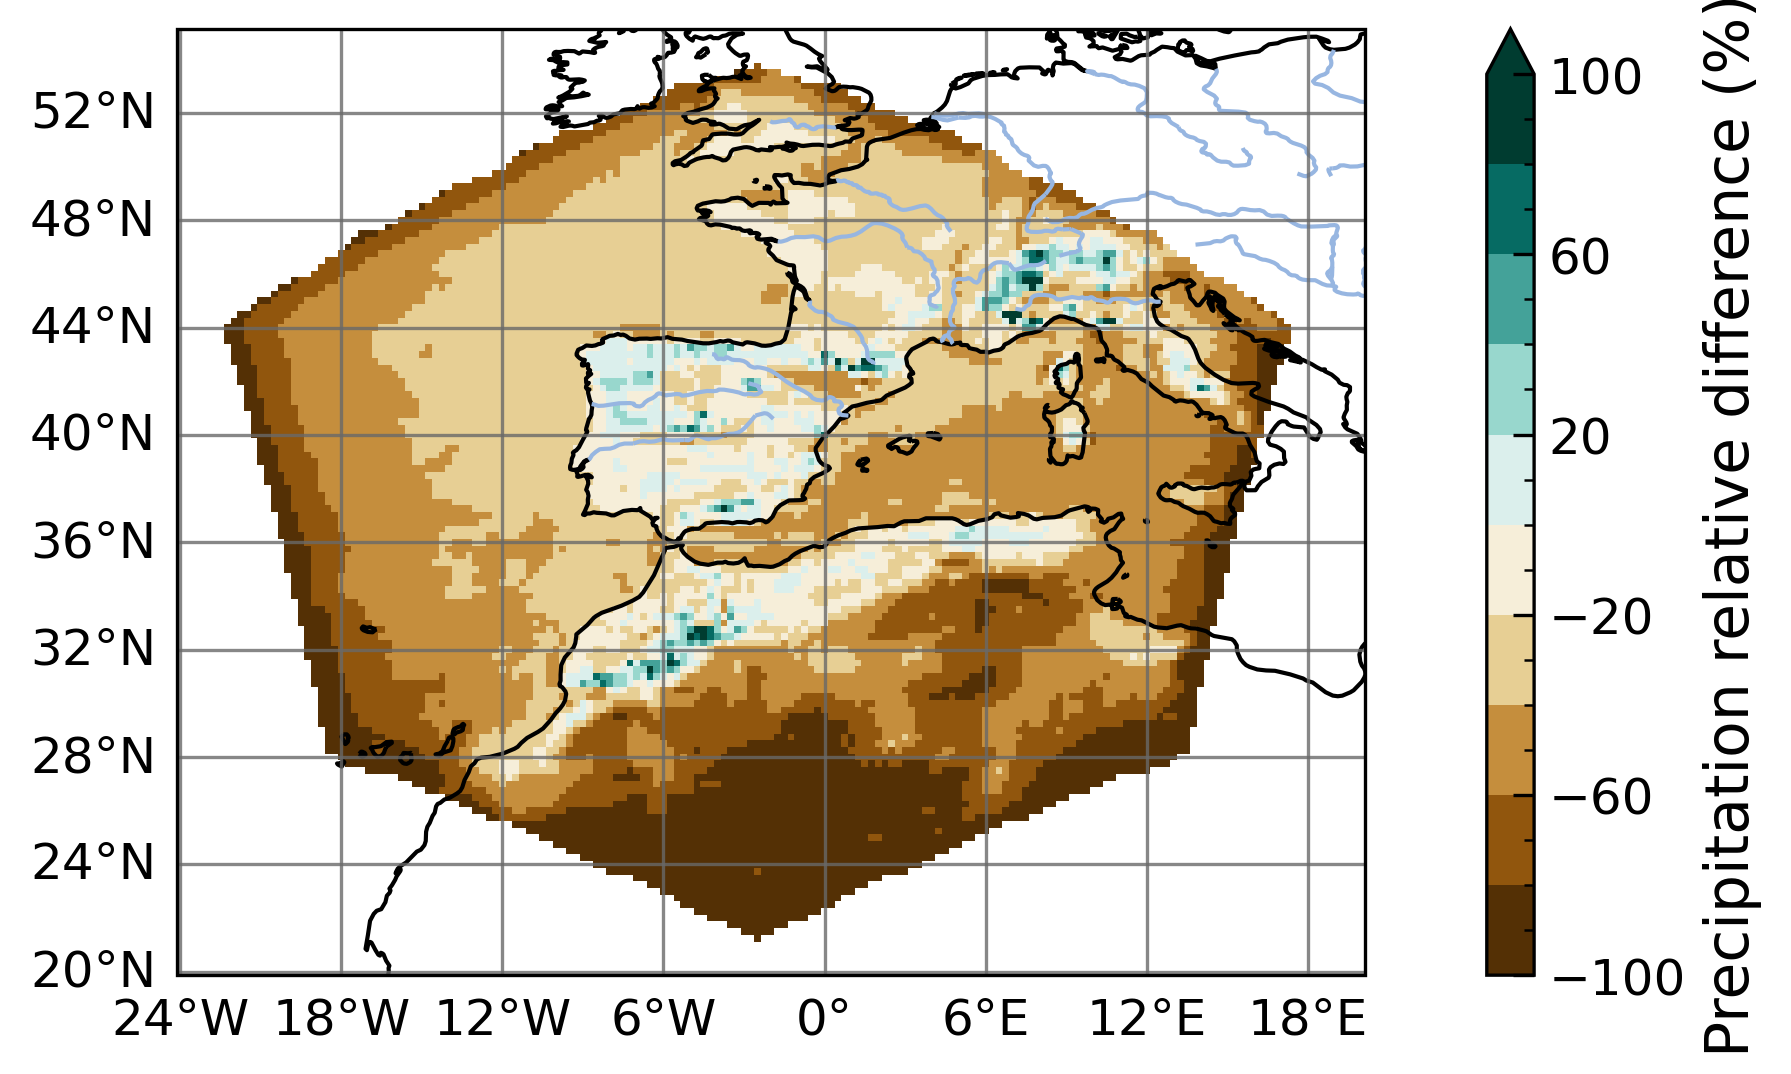
\includegraphics[width=\textwidth]{images/chap4/domain_size/rel_diff_map_precip_era_LAM_2000km_NBP80.png}
        \end{subfigure} \\
        
        %evap
        \begin{subfigure}[b]{0.33\textwidth}
            \caption{}
            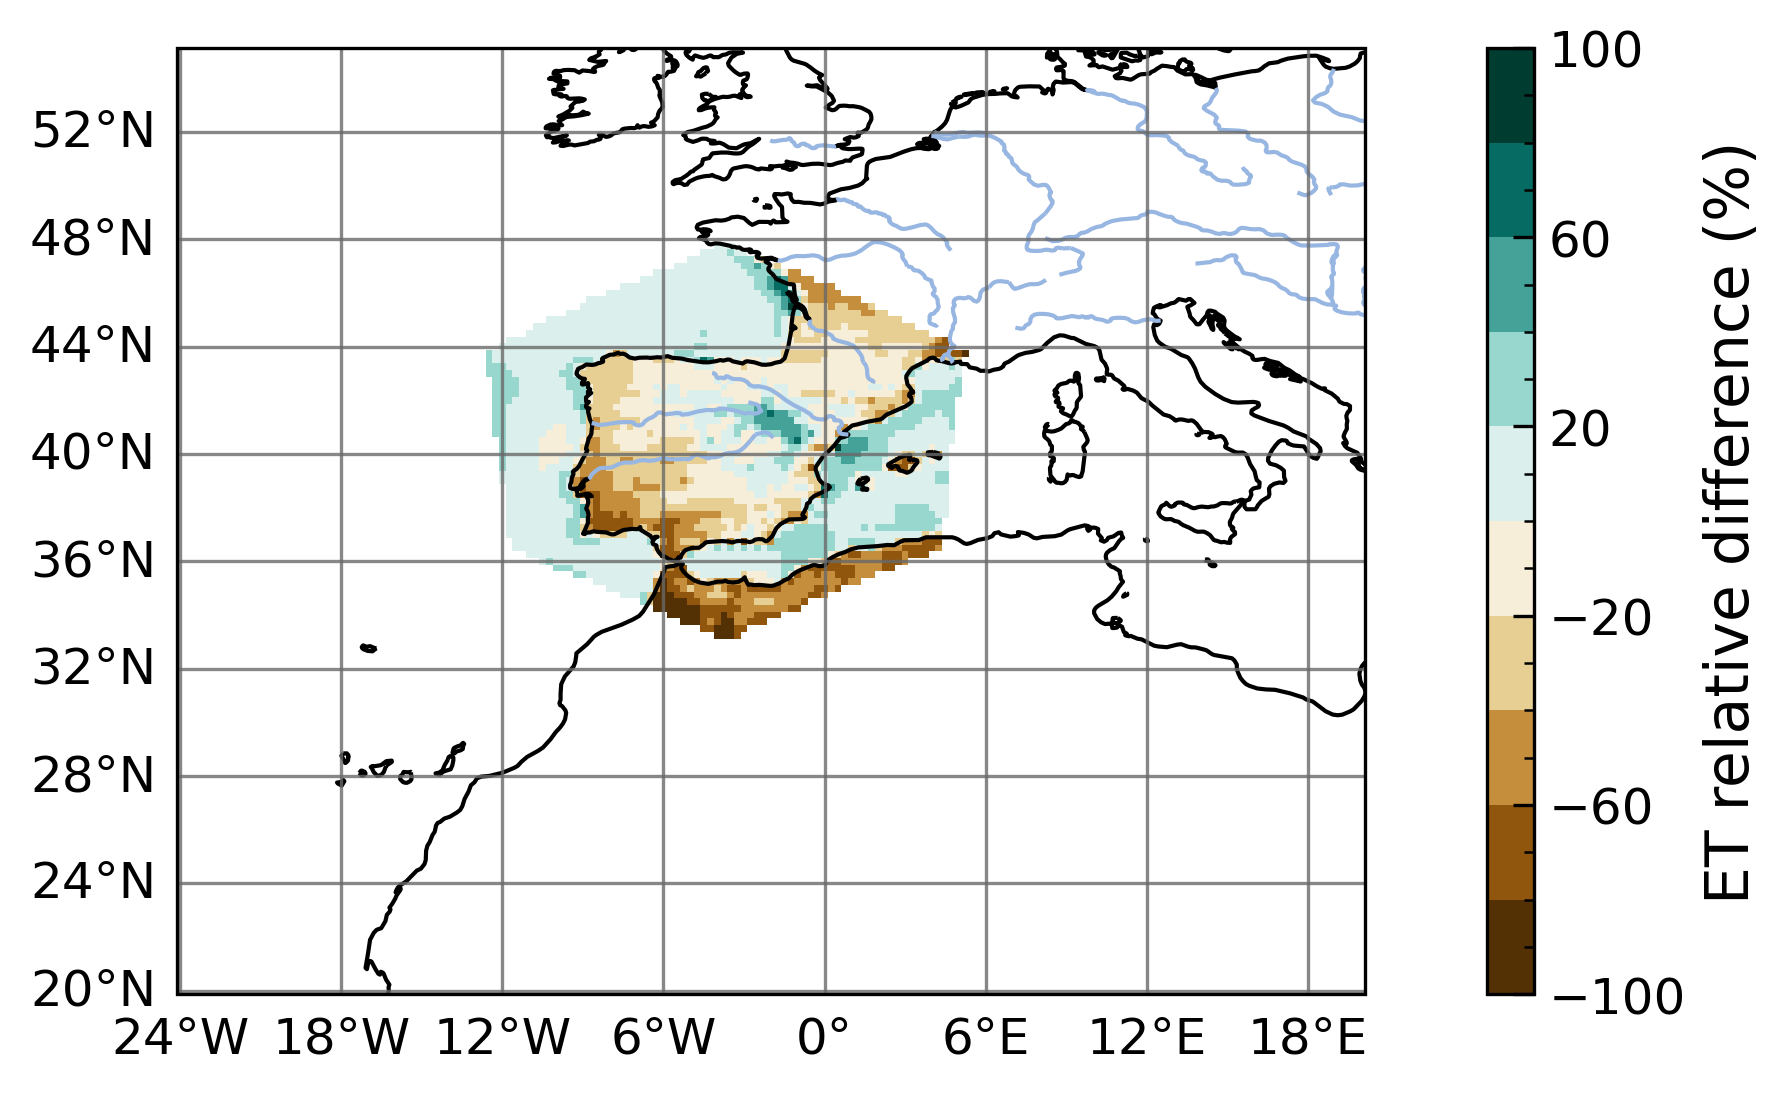
\includegraphics[width=\textwidth]{images/chap4/domain_size/rel_diff_map_evap_era_LAM_1000km_NBP40.png}
        \end{subfigure} &
        \begin{subfigure}[b]{0.33\textwidth}
            \caption{}
            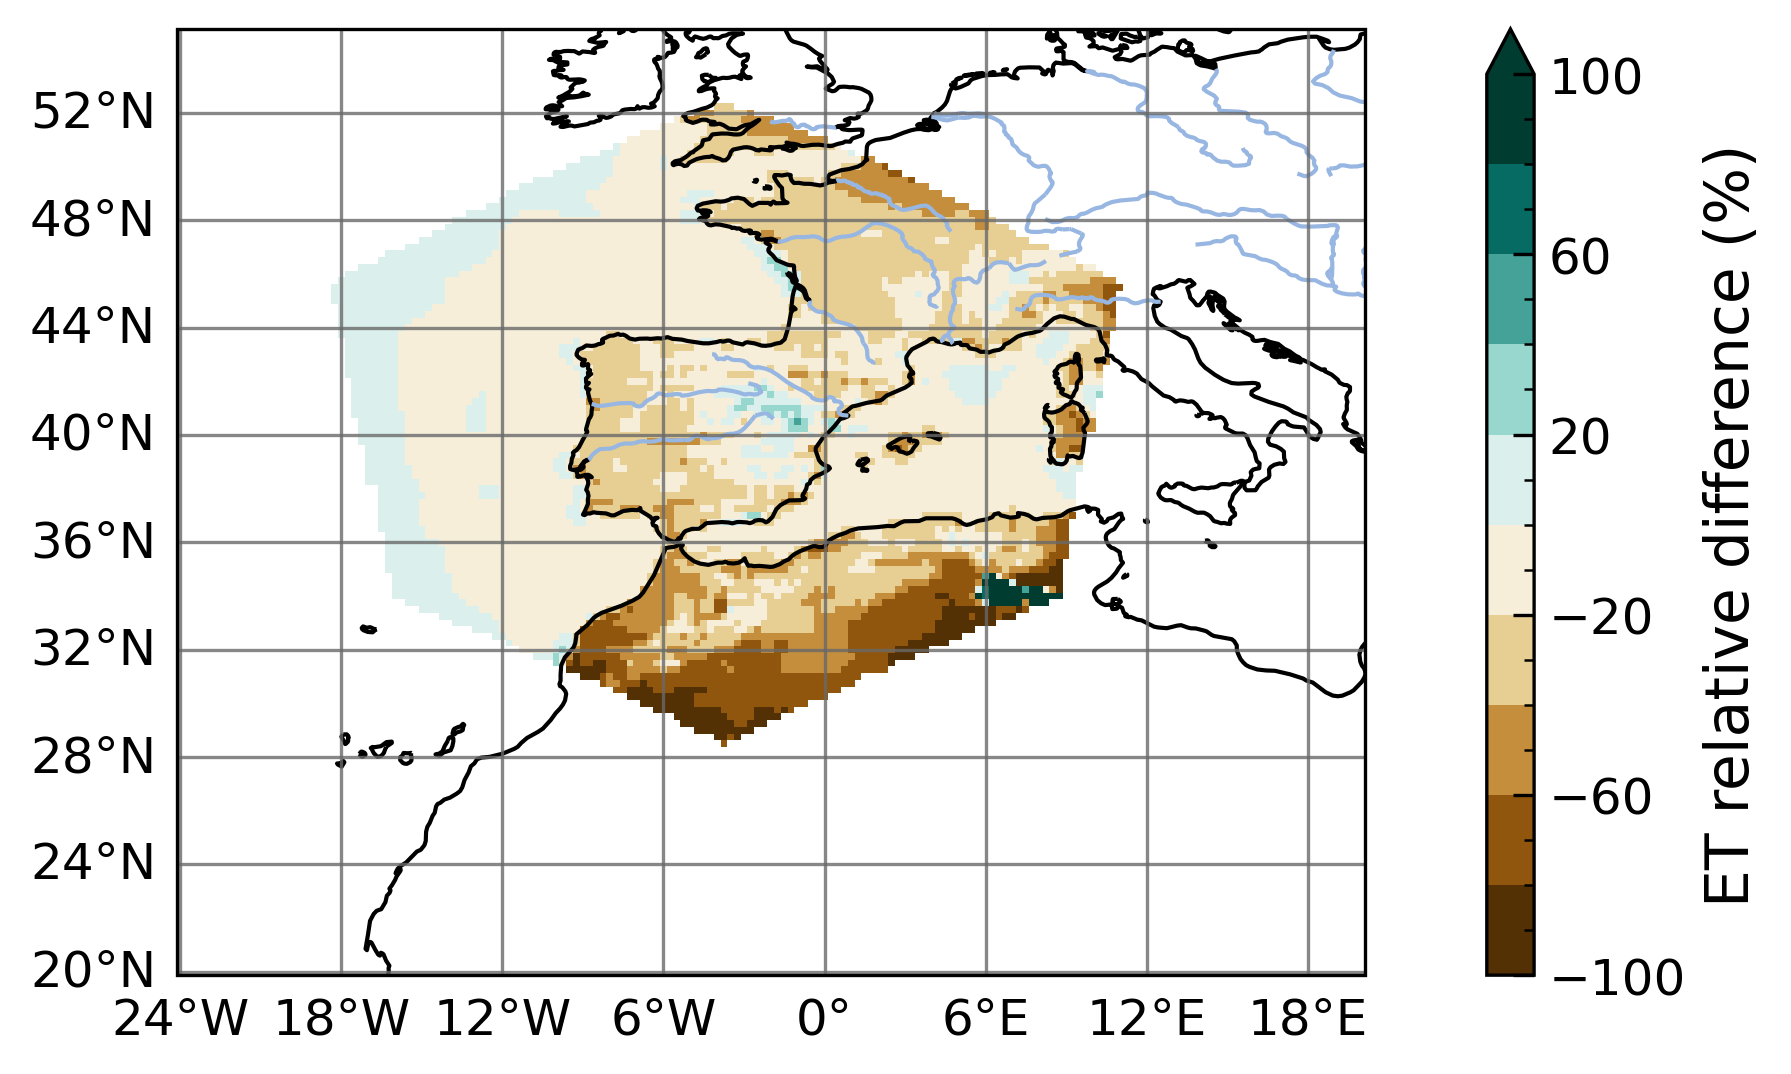
\includegraphics[width=\textwidth]{images/chap4/domain_size/rel_diff_map_evap_era_LAM_1500km_NBP60.png}
        \end{subfigure} &
        \begin{subfigure}[b]{0.33\textwidth}
            \caption{}
            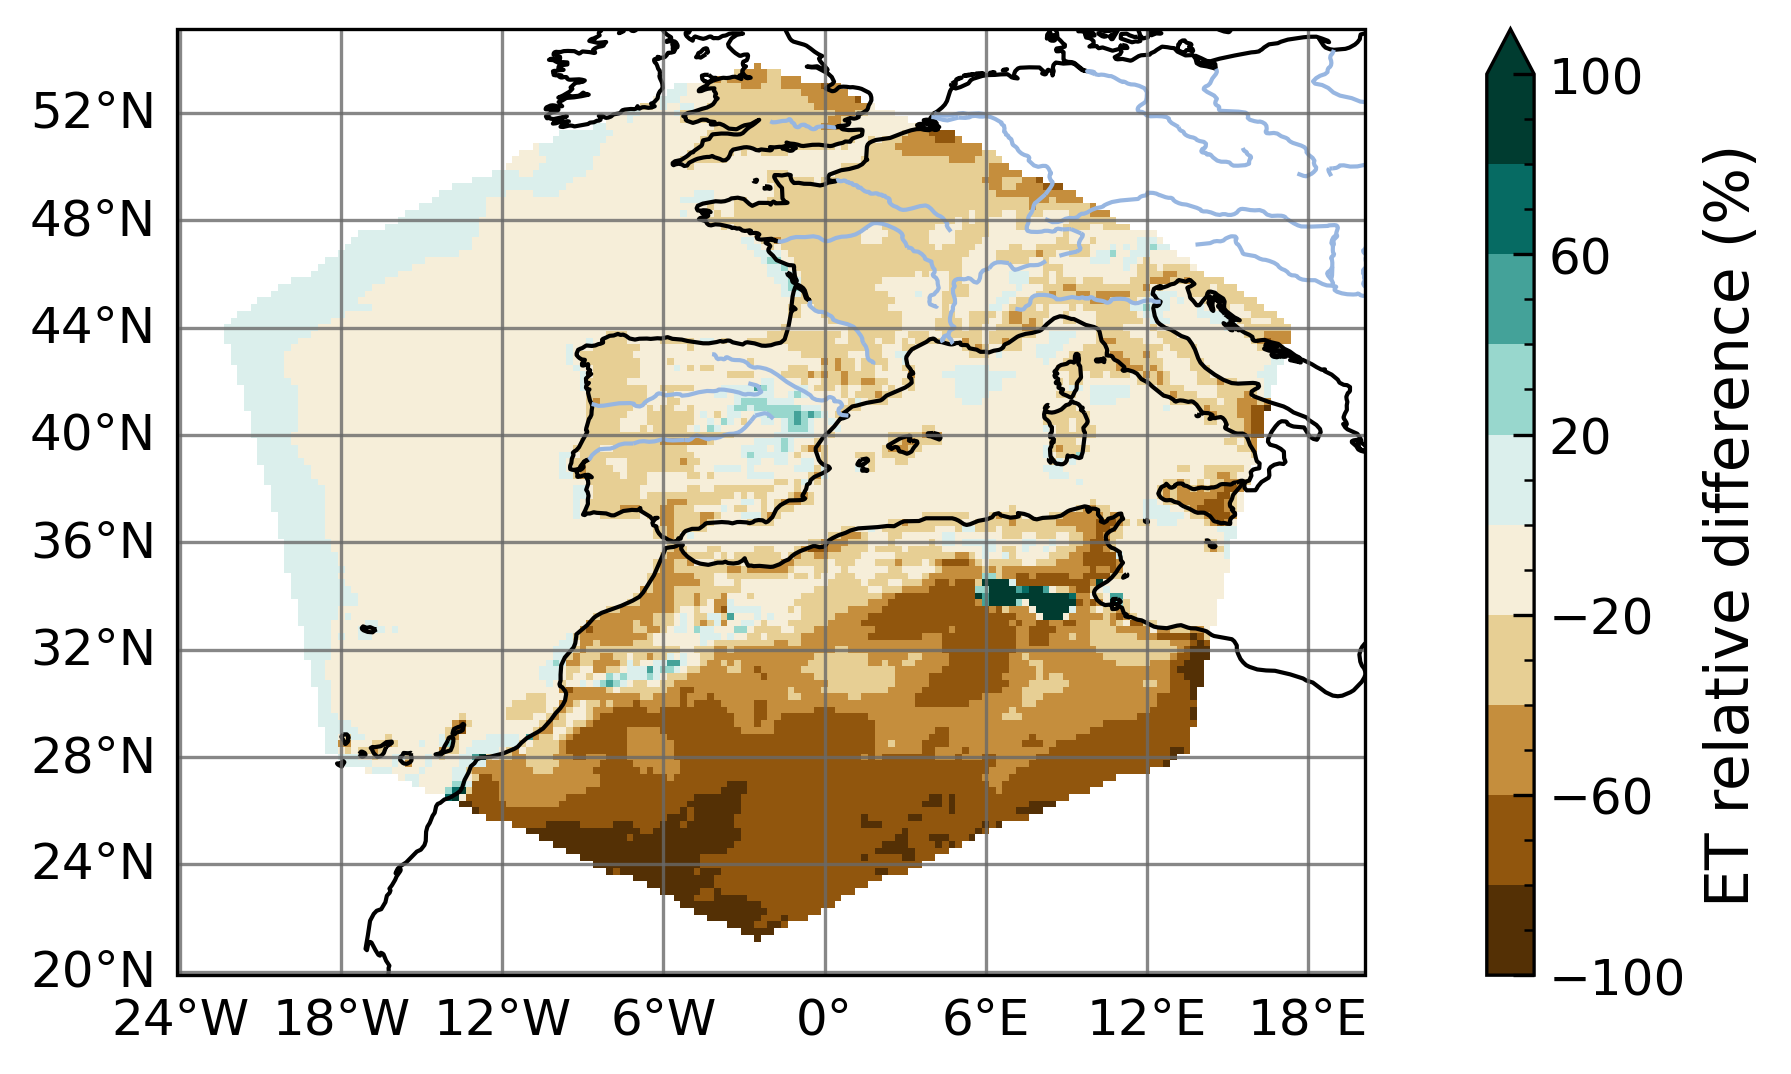
\includegraphics[width=\textwidth]{images/chap4/domain_size/rel_diff_map_evap_era_LAM_2000km_NBP80.png}
        \end{subfigure}
    \end{tabular}
    \caption{}
    \label{fig:domain_size_ERA_reldiff_maps}
\end{figure}

\clearpage
 
\section*{Appendix to chapter \ref{chap:monthly}}
% Article

%f
\begin{figure}[htbp]
    \centering
    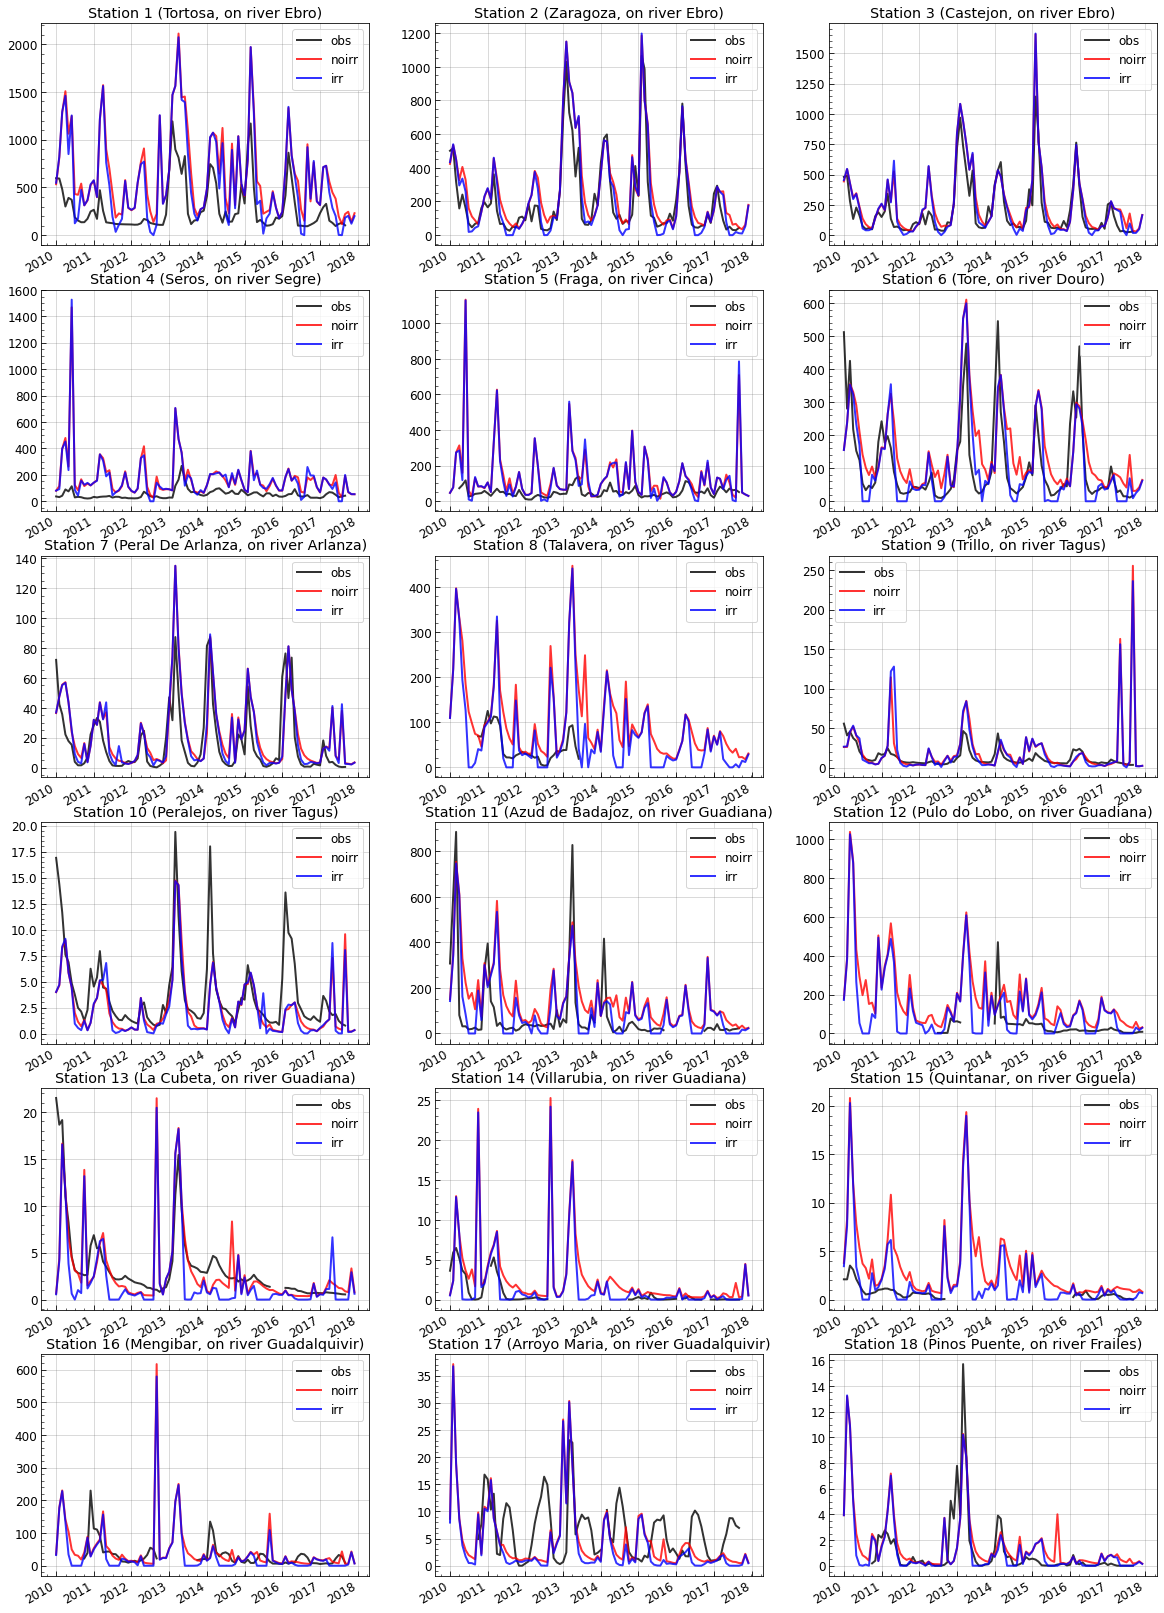
\includegraphics[width=\textwidth]{images/chap4/article/18_stations_TS.png}
    \caption{Time series of river discharge for the \irr and \noirr simulations and GRDC observations.}
    \label{fig:TS_discharge_18stations}
\end{figure}

%f
\begin{figure}[htbp]
    \centering
    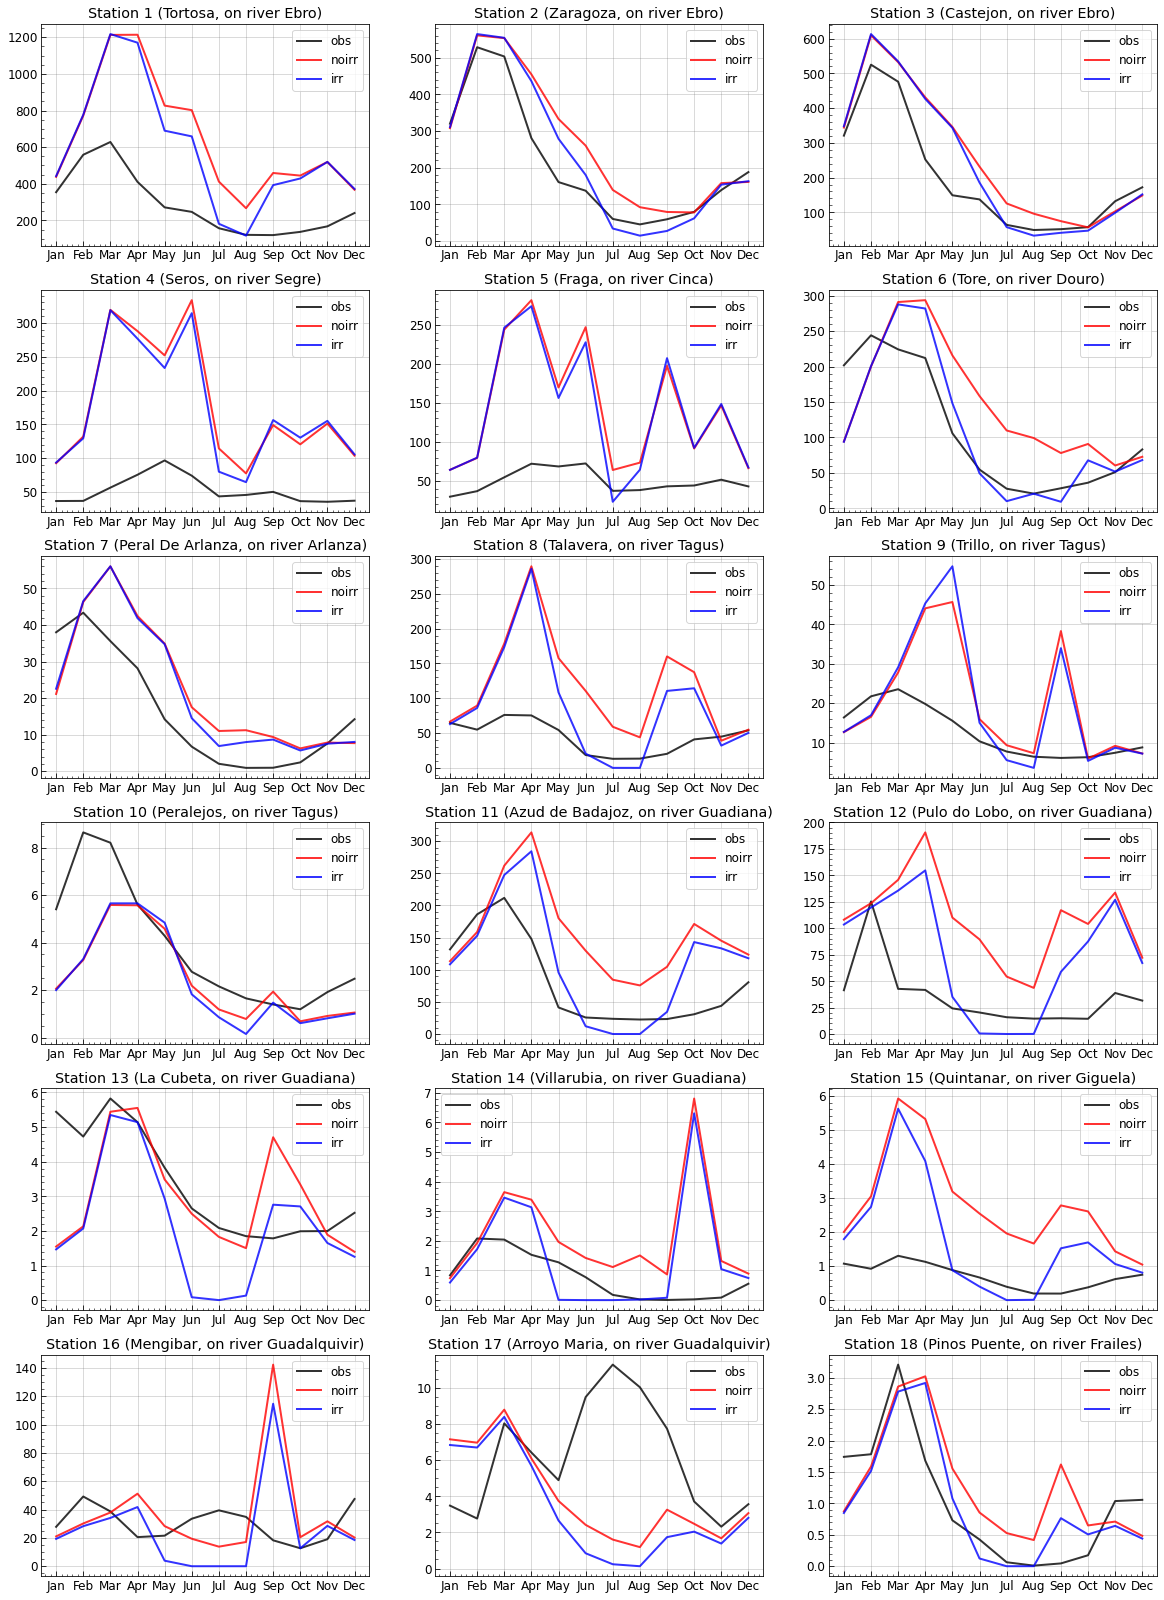
\includegraphics[width=\textwidth]{images/chap4/article/18_stations_SC.png}
    \caption{Mean seasonal cycle of river discharge for the \irr and \noirr simulations and GRDC observations. A mask is applied to the simulations to filter out months without corresponding observation data.}
    \label{fig:SC_discharge_18stations}
\end{figure}


% Climate change 

%figure : from chap 4 future vs present. Seasonnal cycle of variables for 3 sims
\begin{figure}[htbp]
    \centering
    \begin{tabular}{cc}
        %precip
        \begin{subfigure}[b]{0.5\textwidth}
            \caption{}
            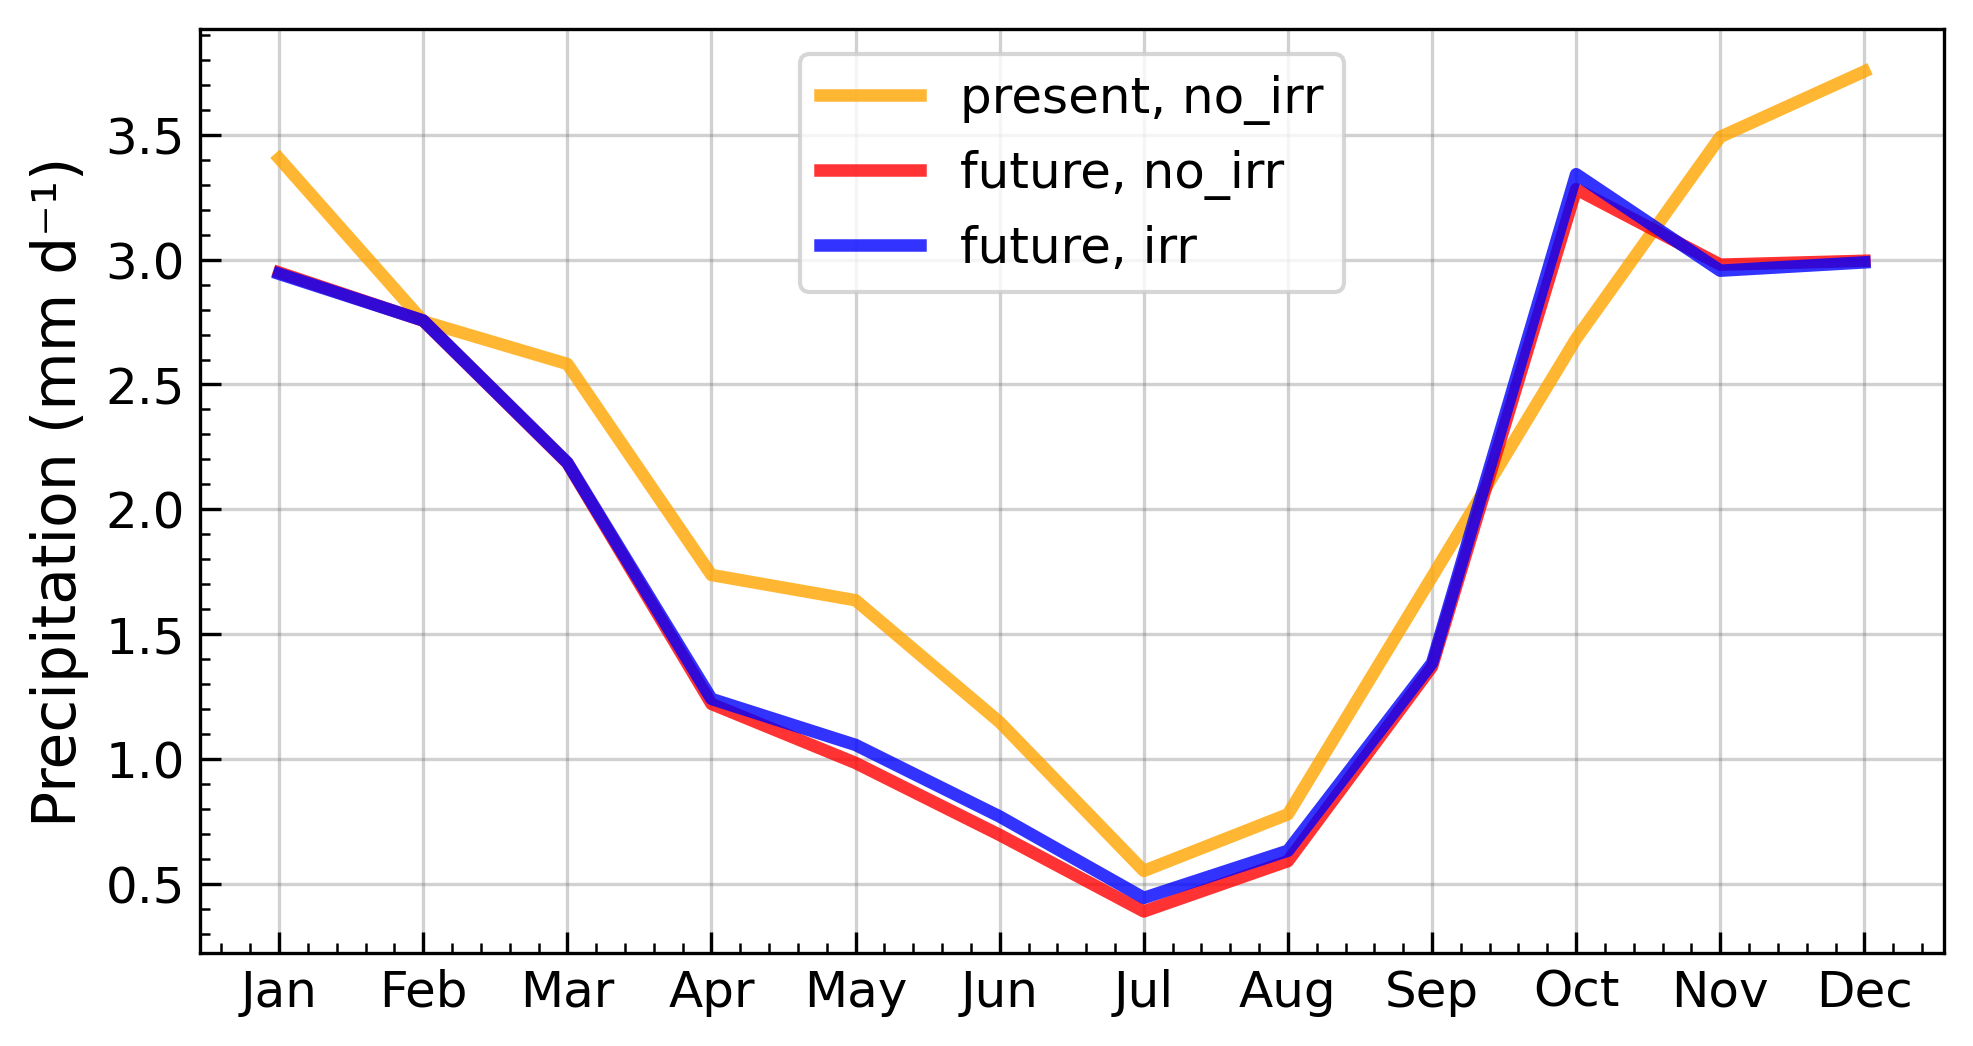
\includegraphics[width=\textwidth]{images/chap4/future/SC_precip_presfutirr.png}
        \end{subfigure} &
        %evap
        \begin{subfigure}[b]{0.5\textwidth}
            \caption{}
            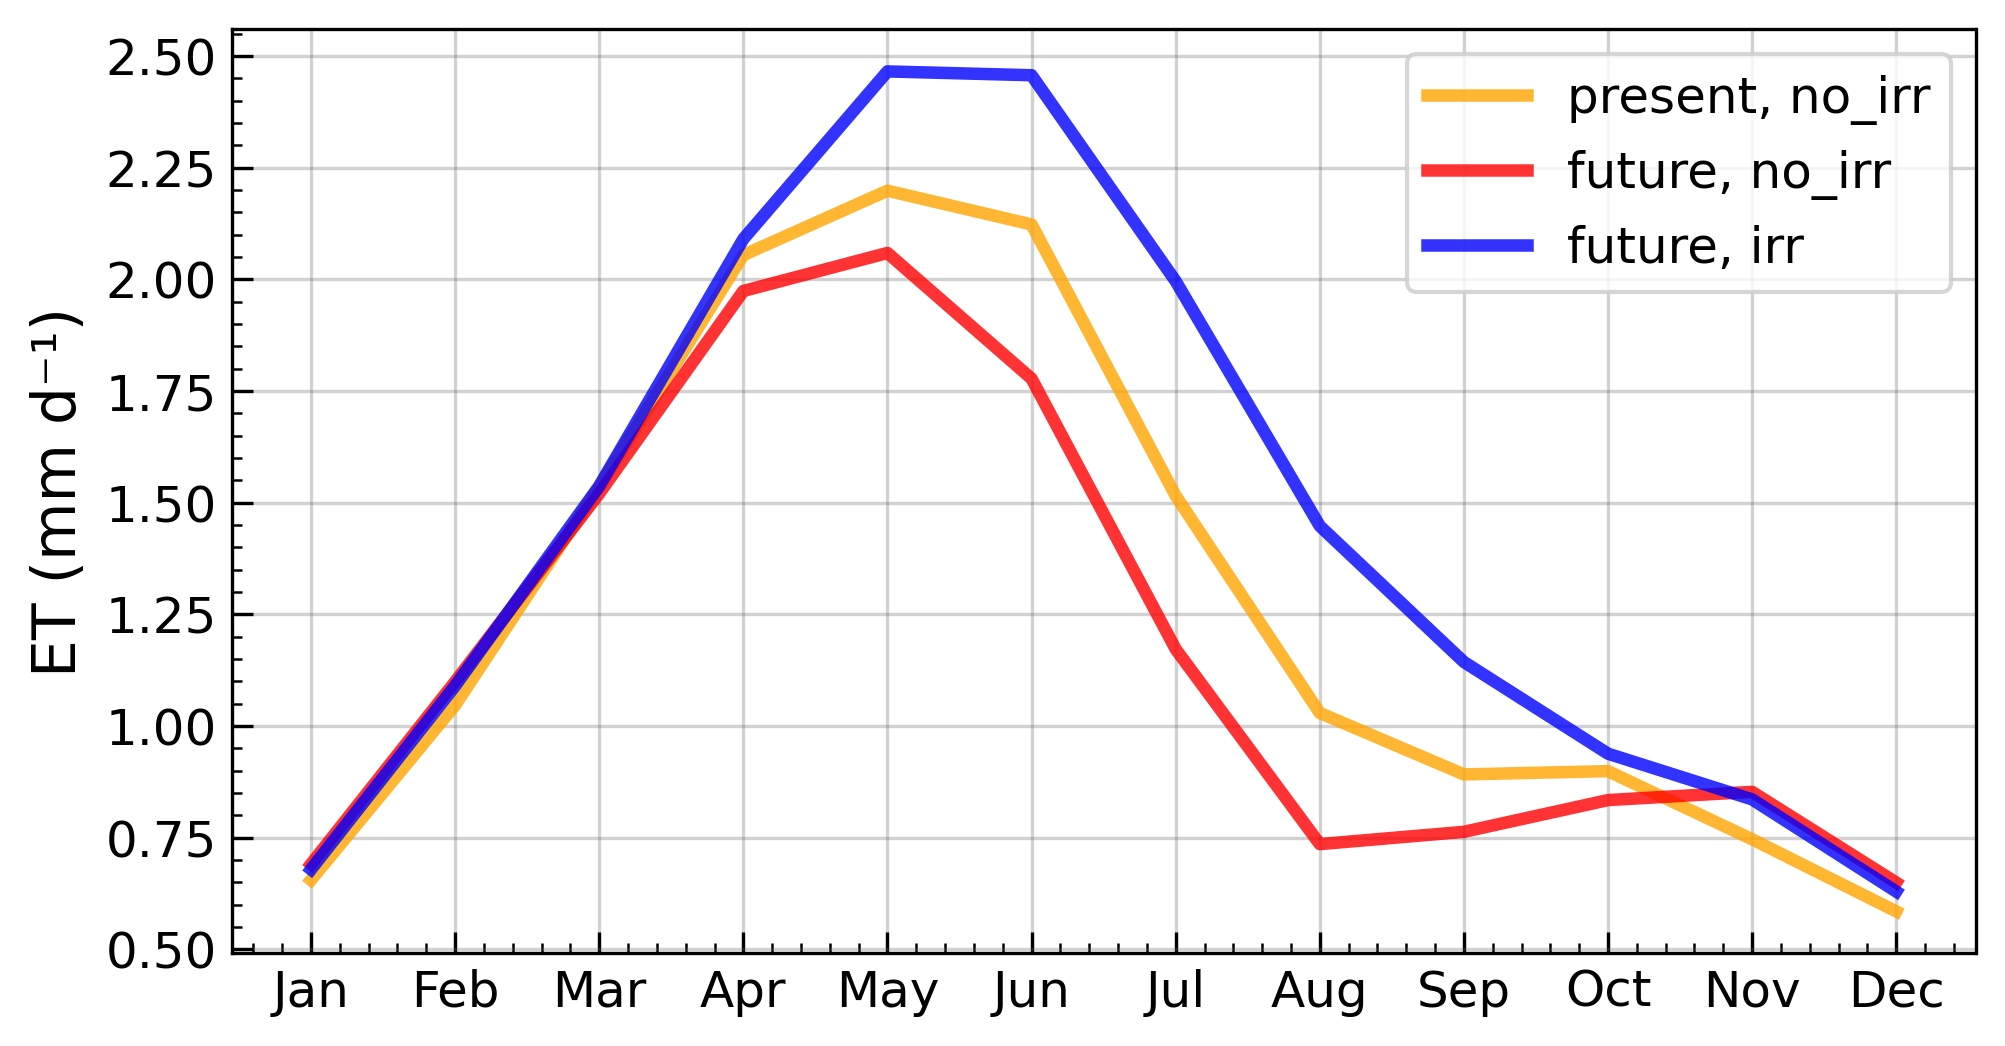
\includegraphics[width=\textwidth]{images/chap4/future/SC_evap_presfutirr.png}
        \end{subfigure} \\

        %t2m
        \begin{subfigure}[b]{0.5\textwidth}
            \caption{}
            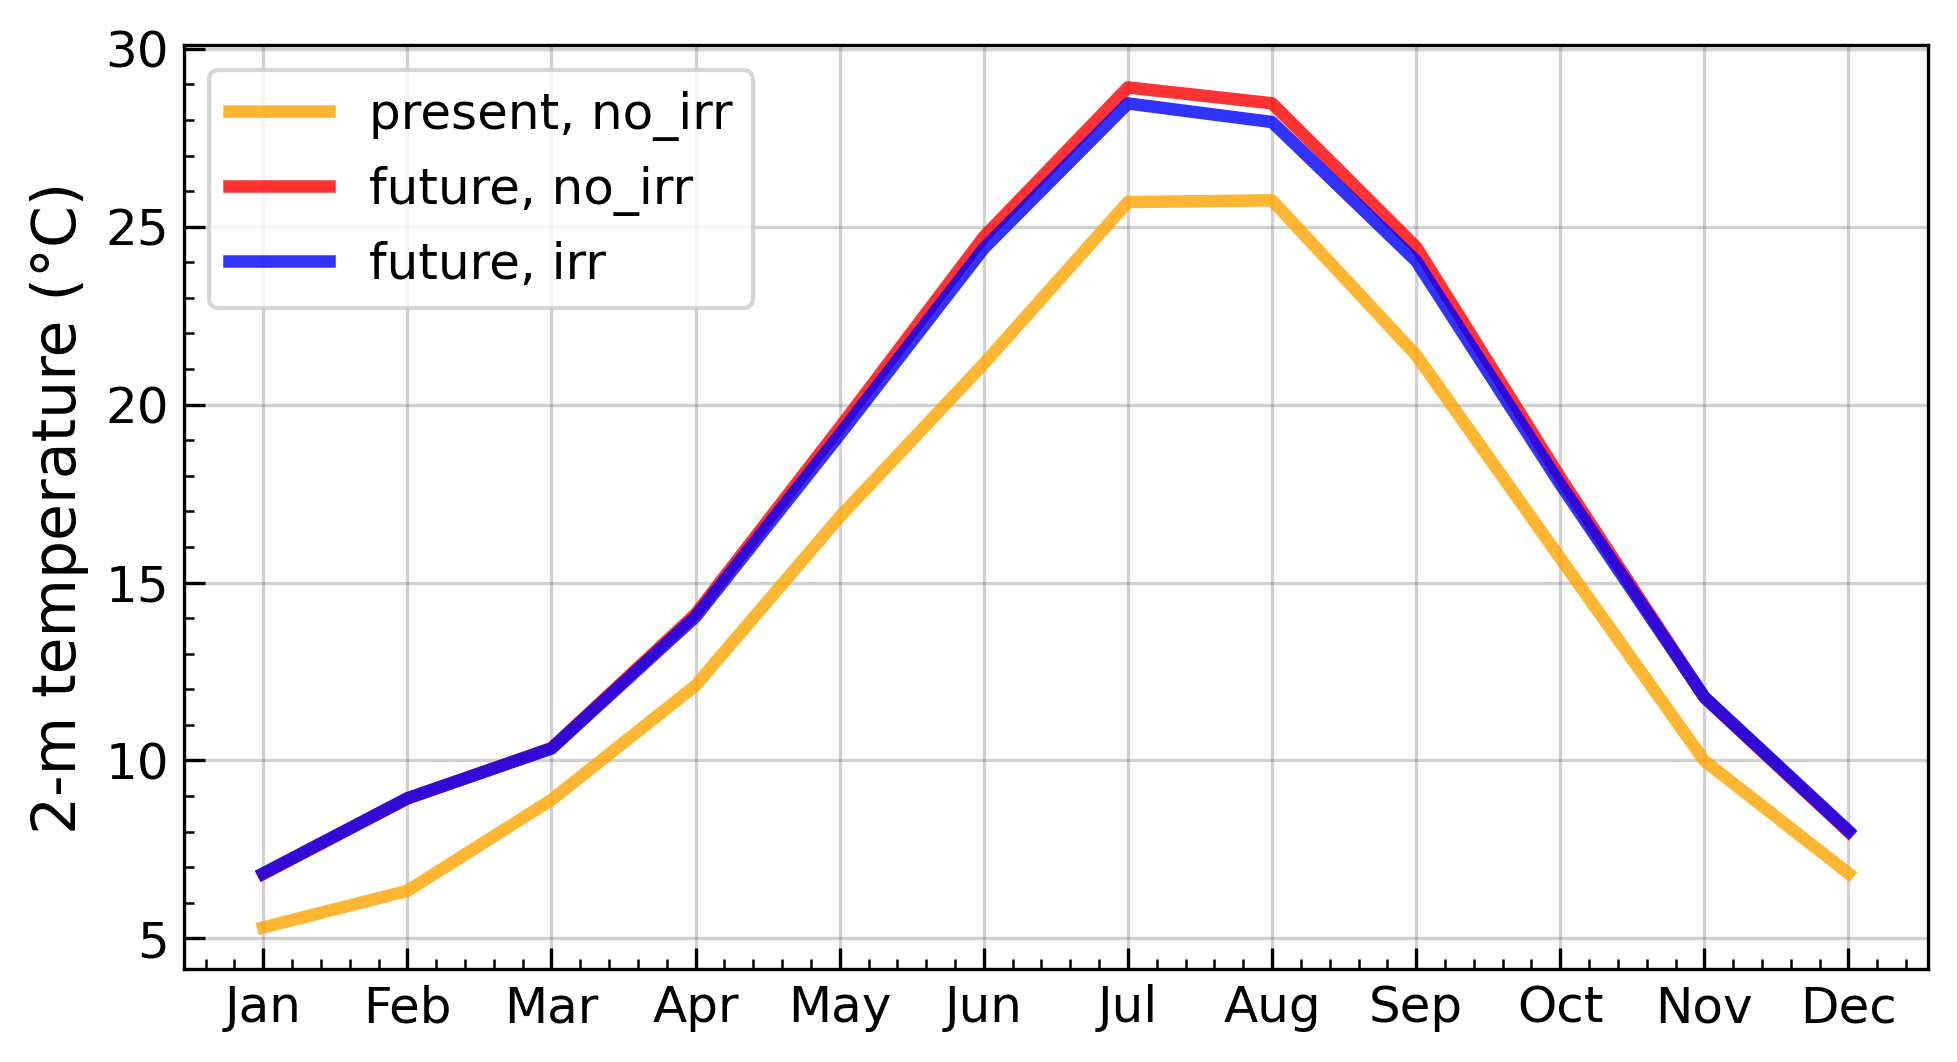
\includegraphics[width=\textwidth]{images/chap4/future/SC_t2m_presfutirr.png}
        \end{subfigure} &
        %fluxsens
        \begin{subfigure}[b]{0.5\textwidth}
            \caption{}
            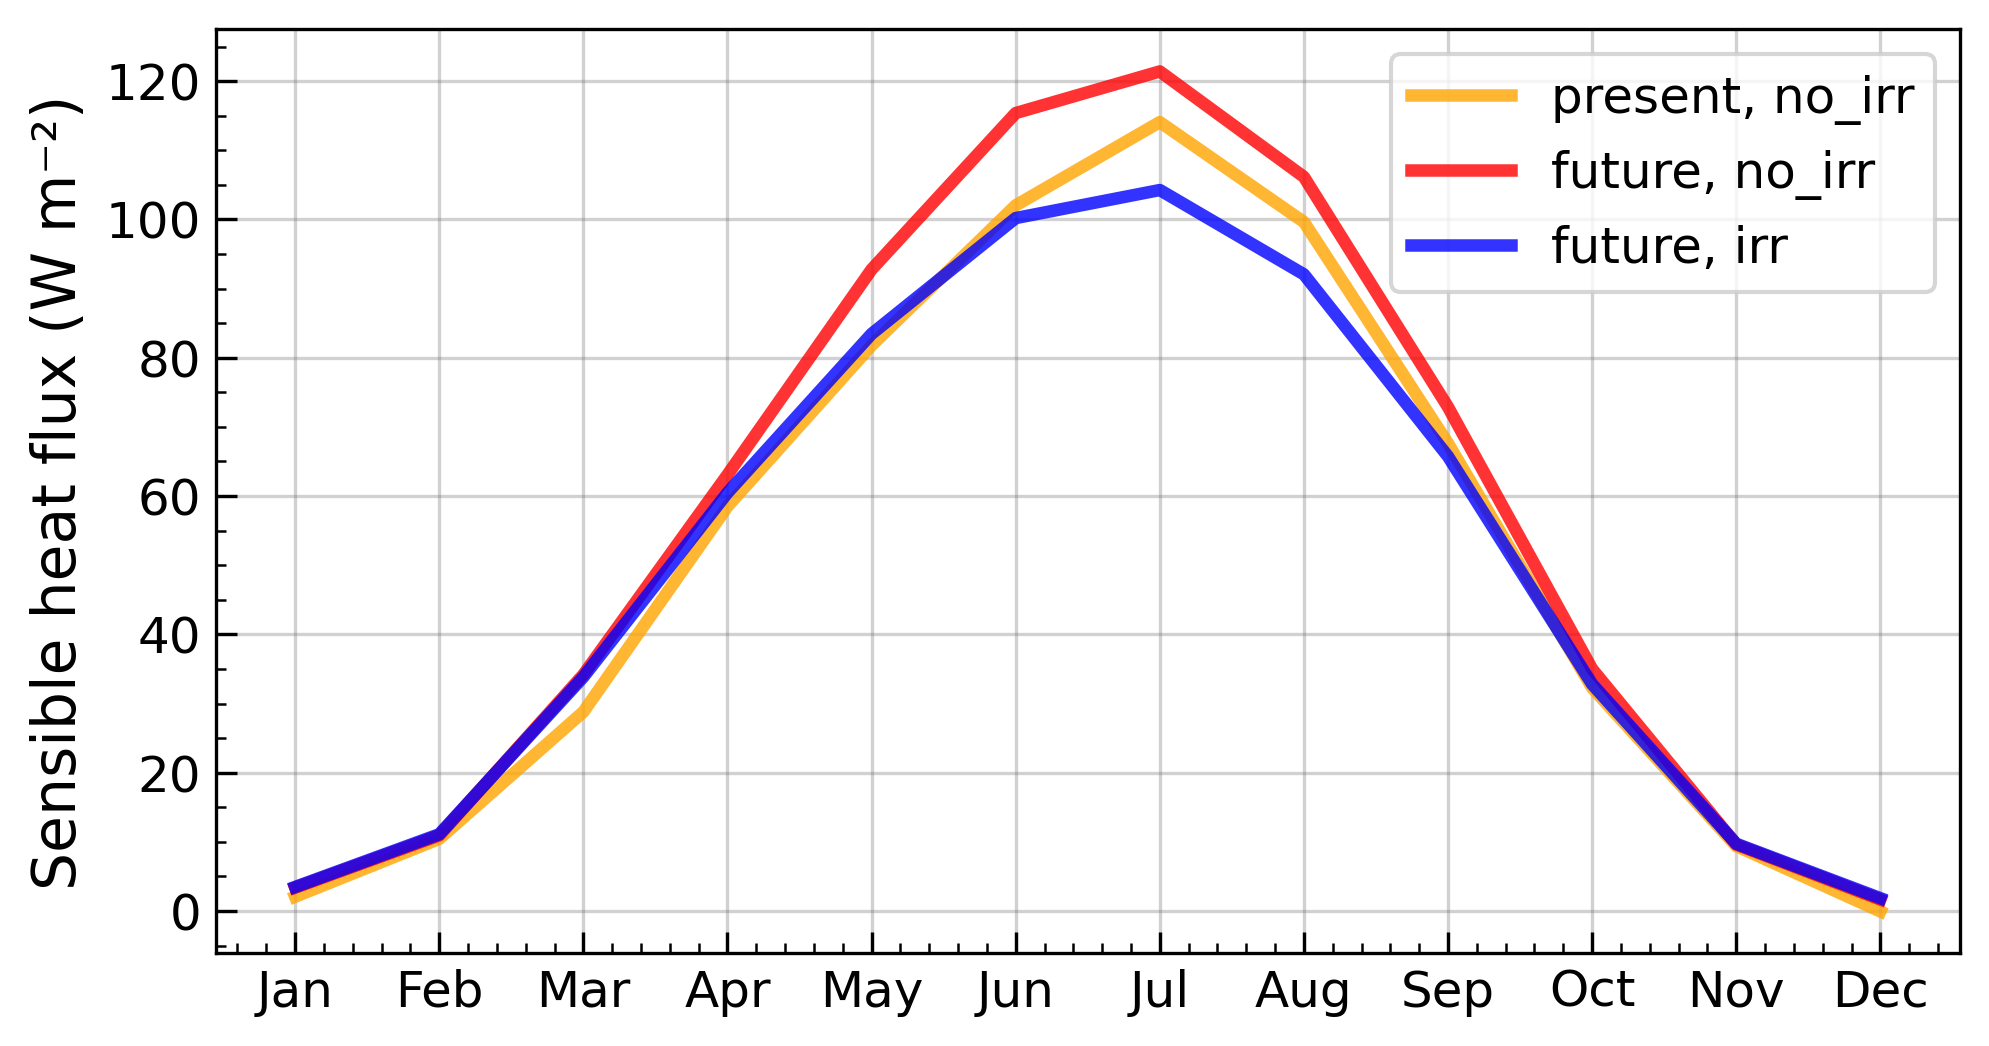
\includegraphics[width=\textwidth]{images/chap4/future/SC_fluxsens_presfutirr.png}
        \end{subfigure} \\

        %q2m
        \begin{subfigure}[b]{0.5\textwidth}
            \caption{}
            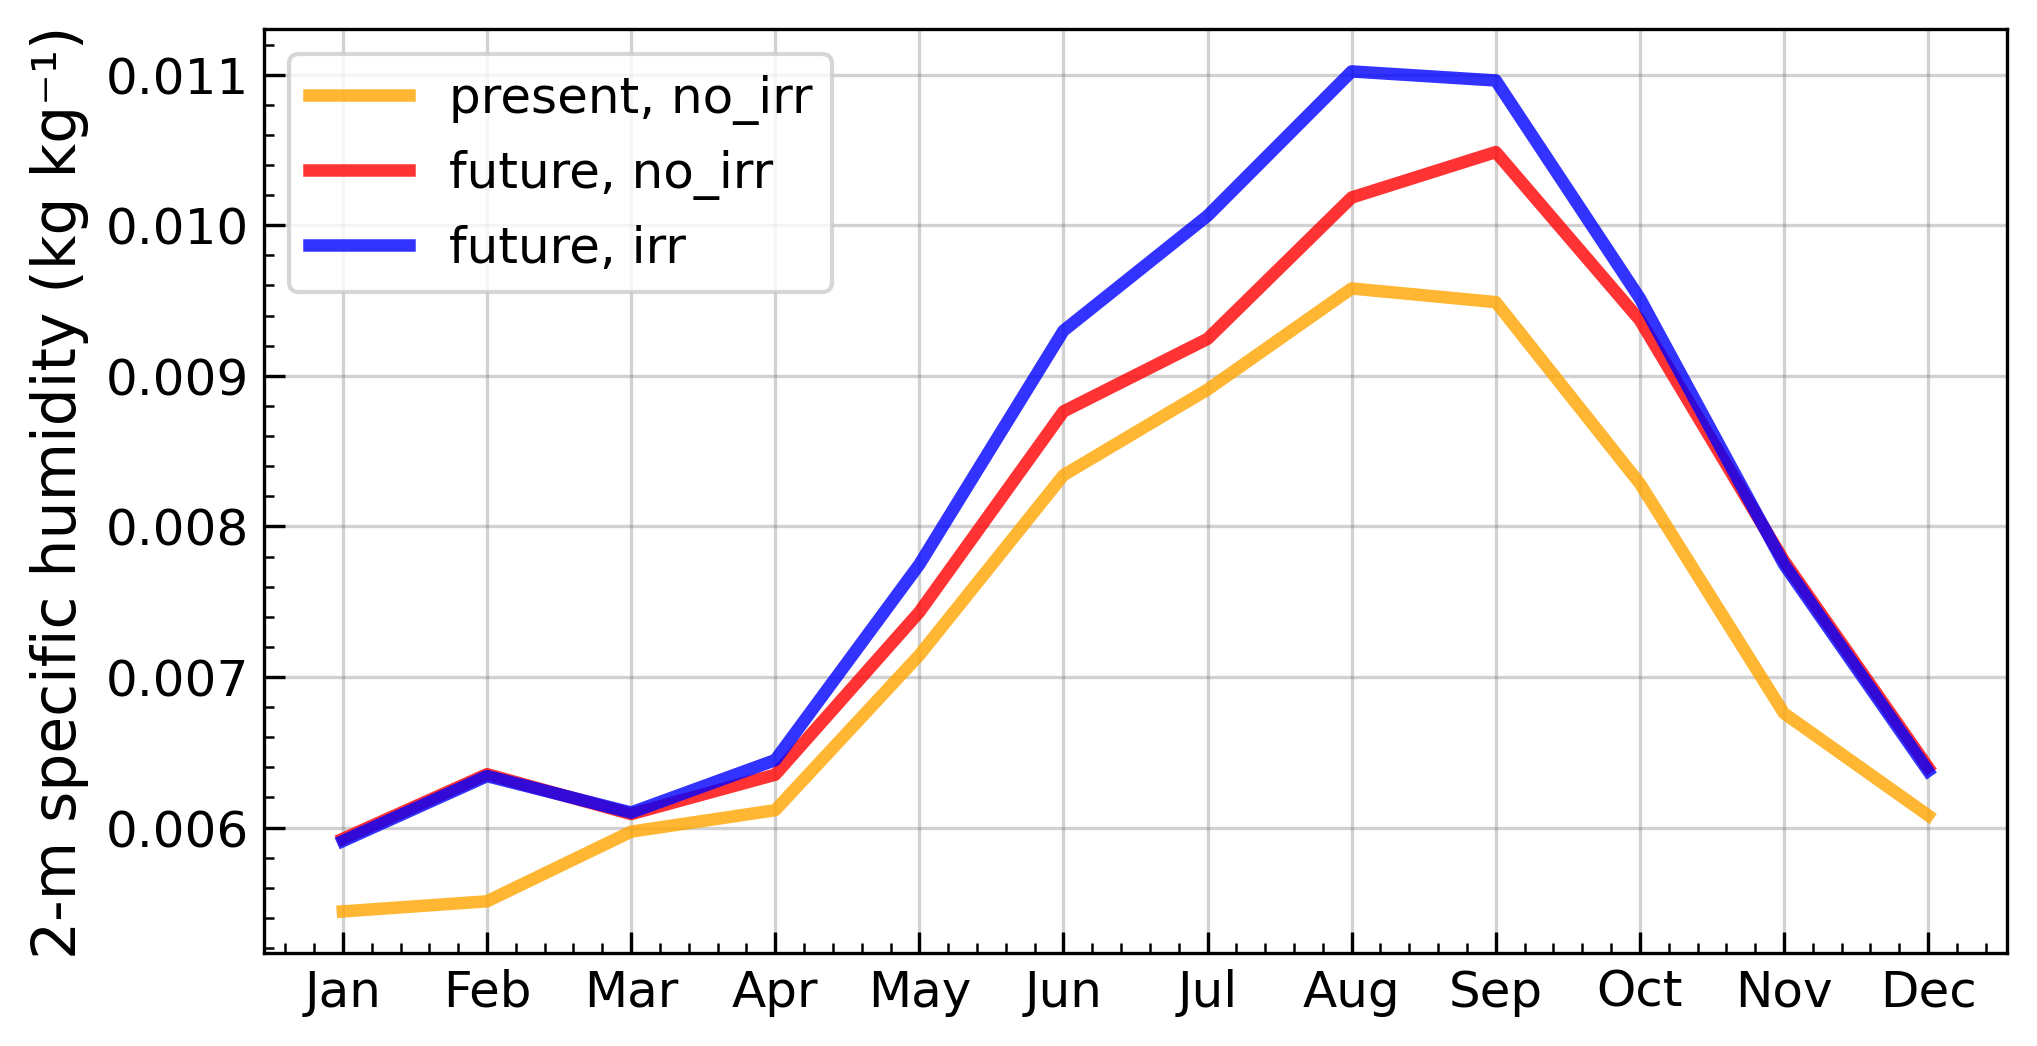
\includegraphics[width=\textwidth]{images/chap4/future/SC_q2m_presfutirr.png}
        \end{subfigure} &
        %rh2m
        \begin{subfigure}[b]{0.5\textwidth}
            \caption{}
            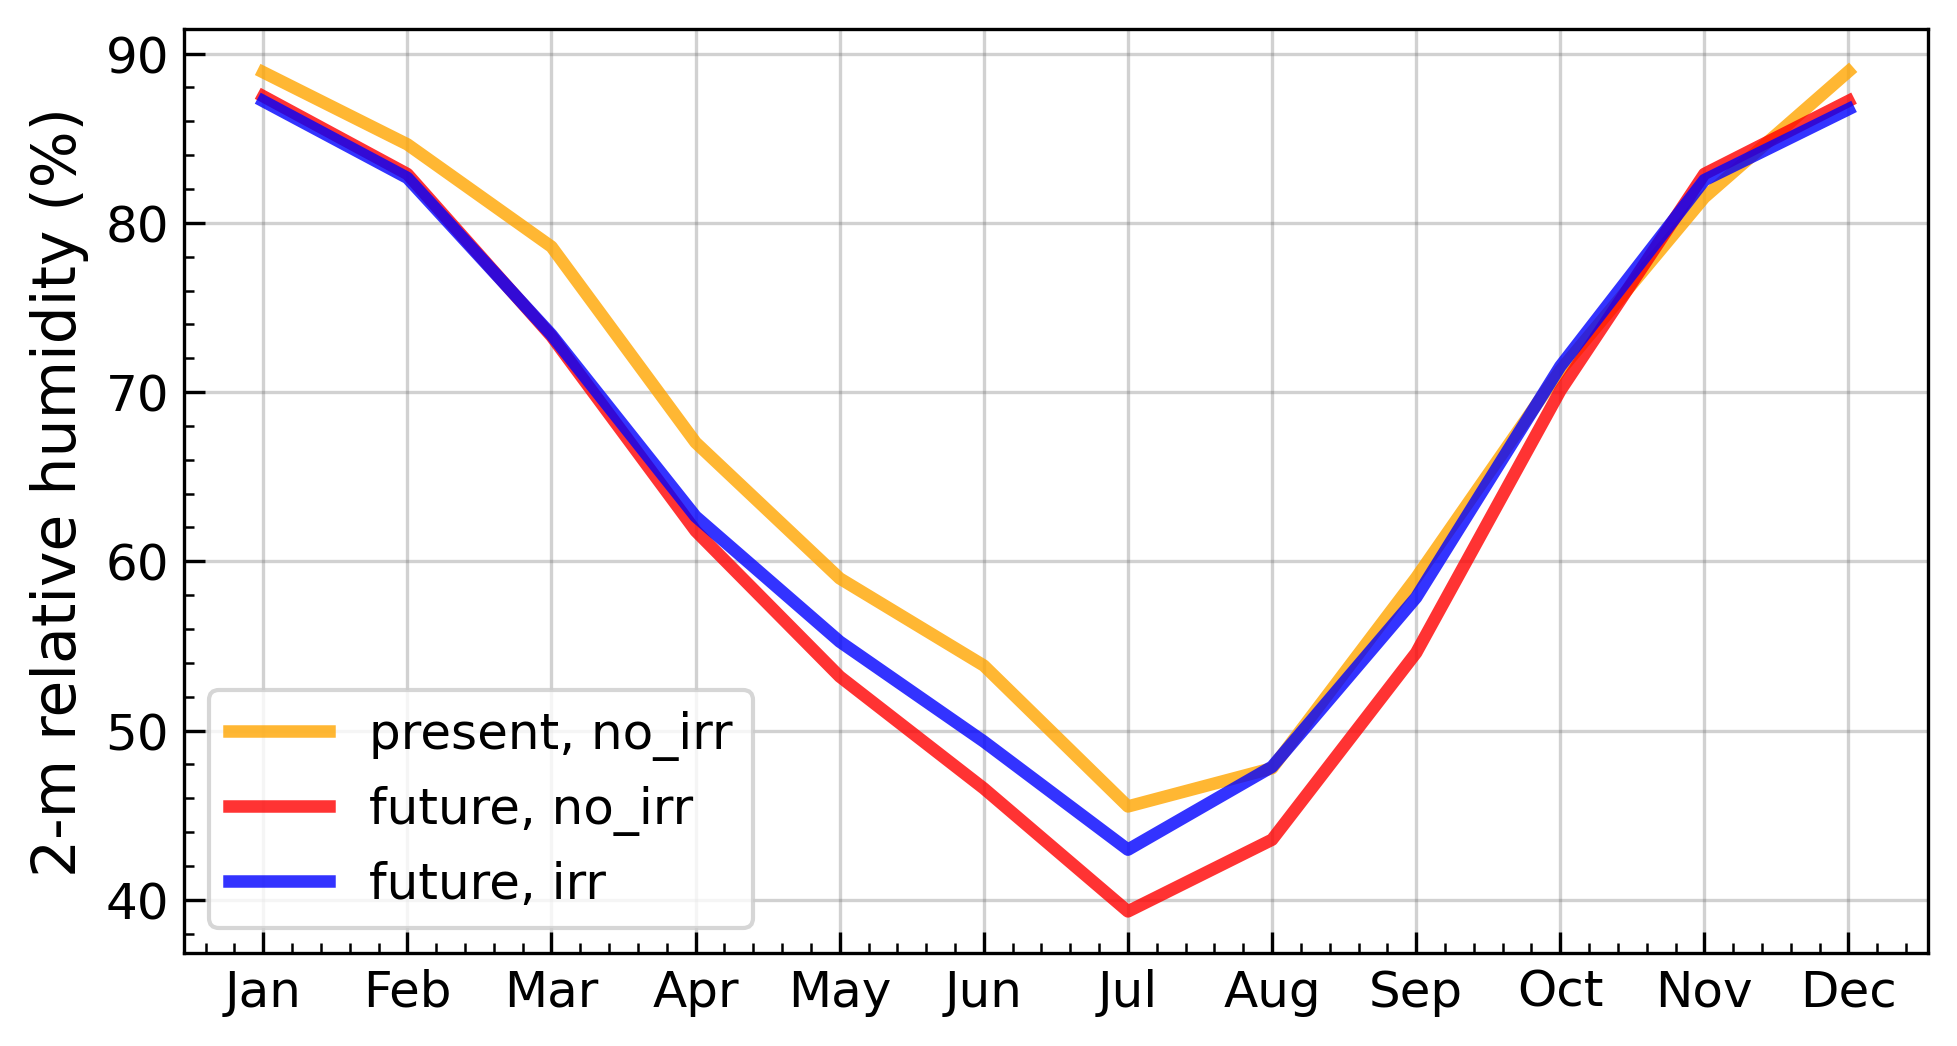
\includegraphics[width=\textwidth]{images/chap4/future/SC_rh2m_presfutirr.png}
        \end{subfigure} \\

        %pblh
        \begin{subfigure}[b]{0.5\textwidth}
            \caption{}
            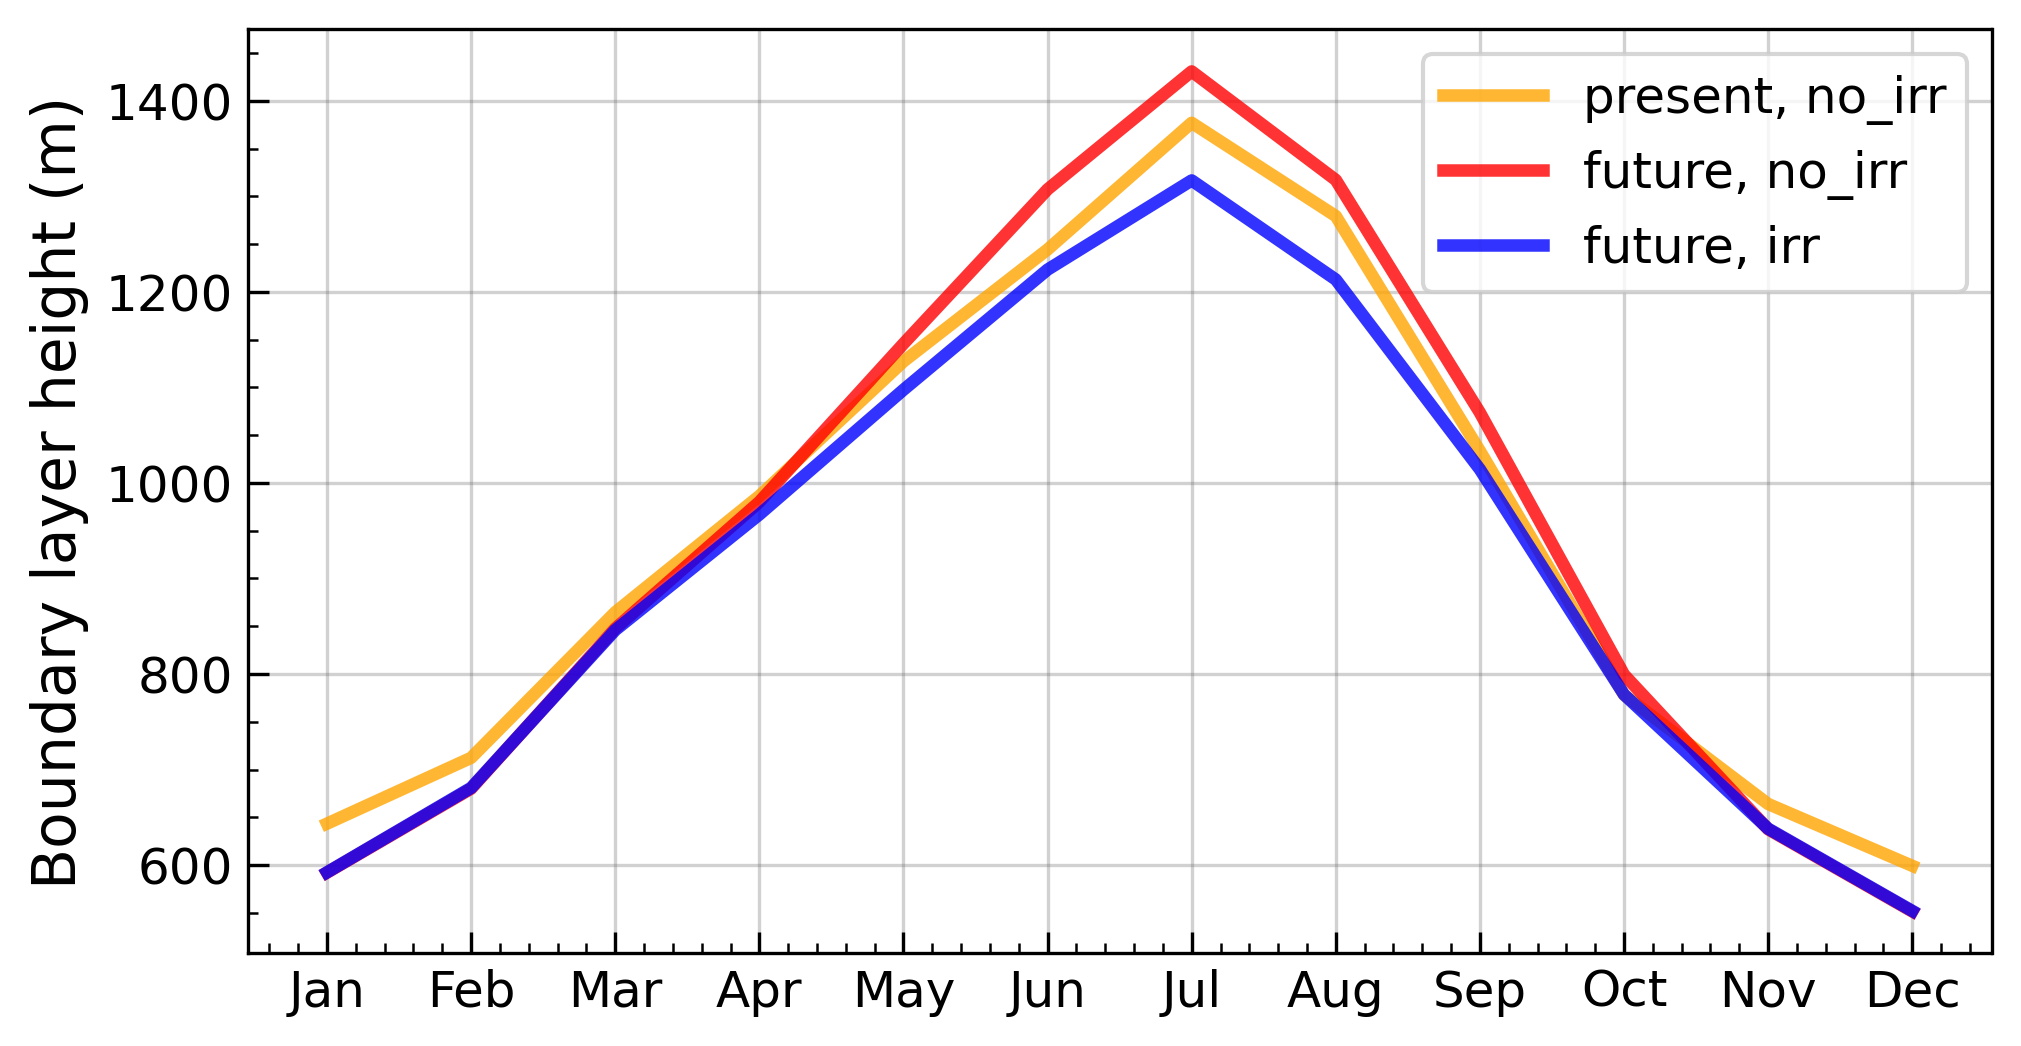
\includegraphics[width=\textwidth]{images/chap4/future/SC_s_pblh_presfutirr.png}
        \end{subfigure} &
        %lcl
        \begin{subfigure}[b]{0.5\textwidth}
            \caption{}
            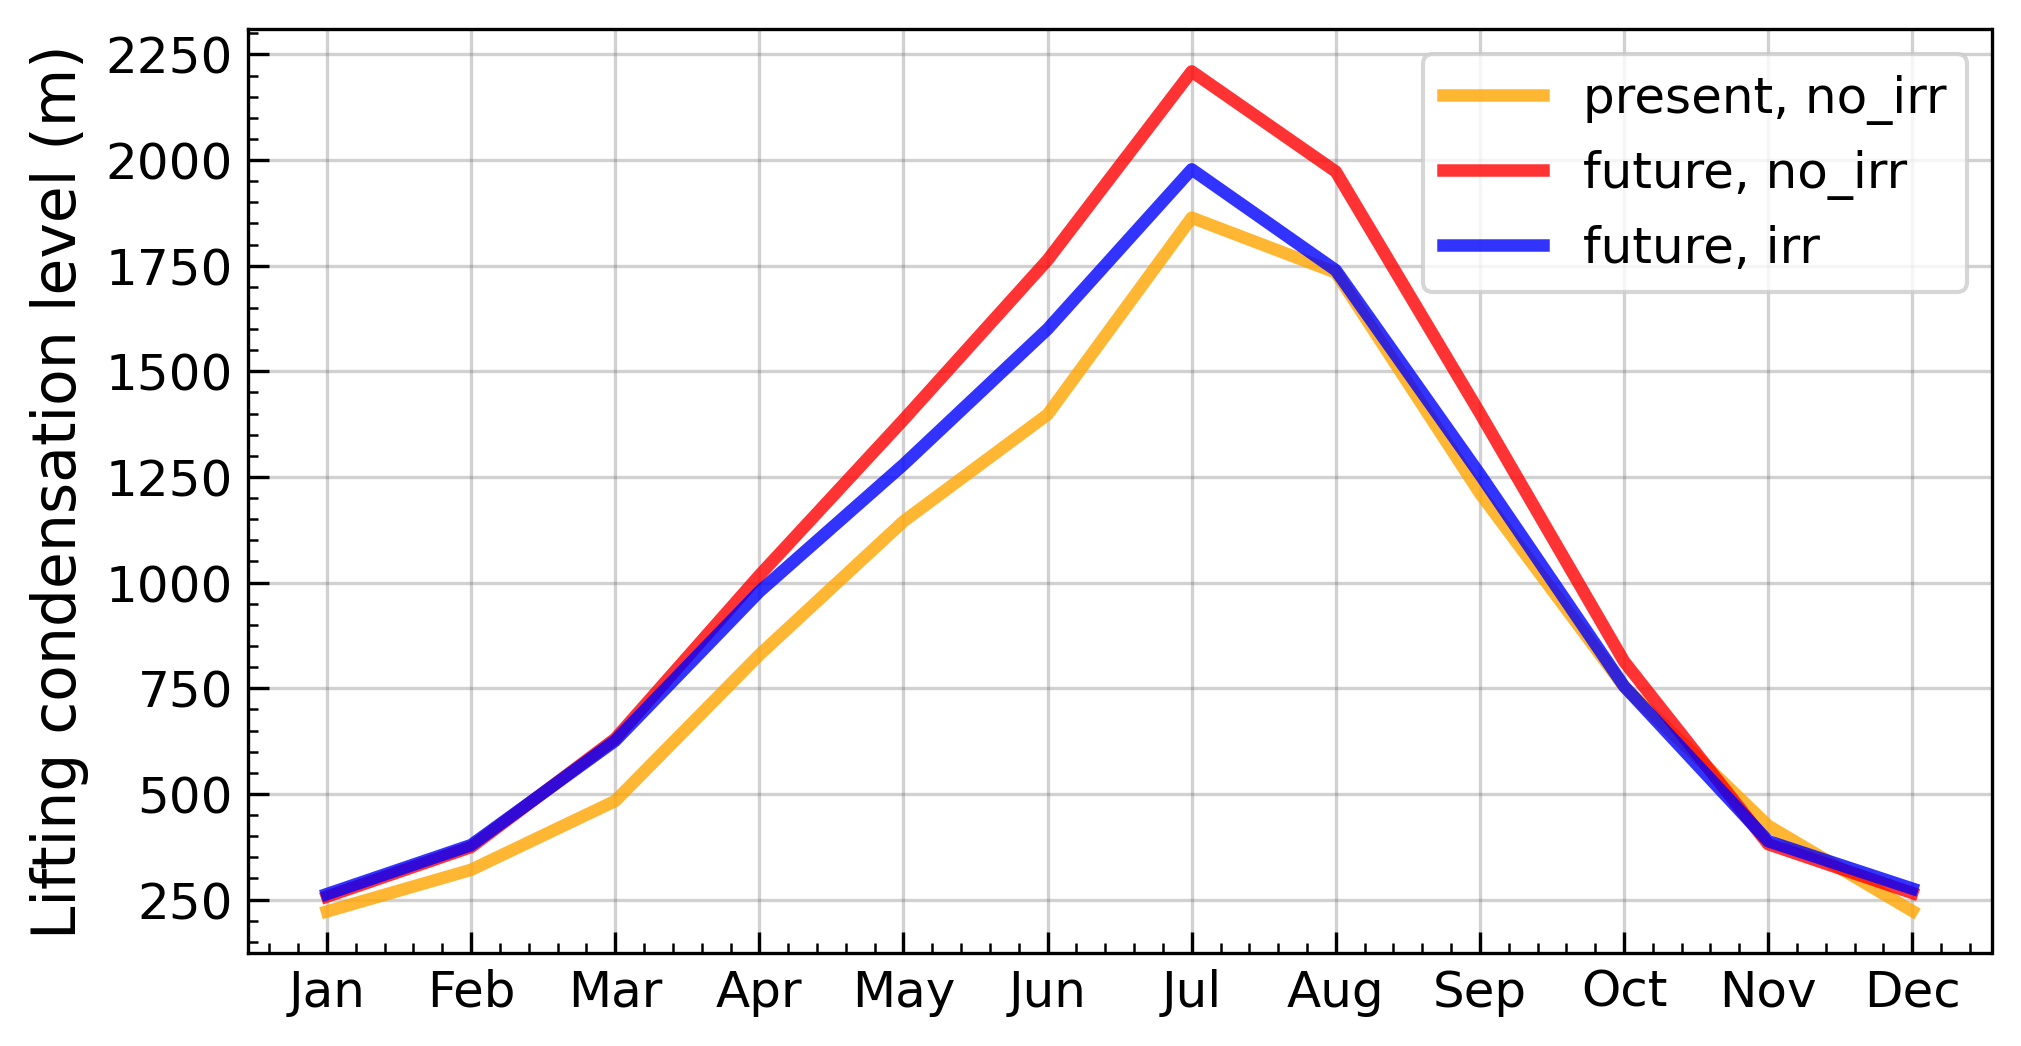
\includegraphics[width=\textwidth]{images/chap4/future/SC_s_lcl_presfutirr.png}
        \end{subfigure} \\
    \end{tabular}
    \caption{}
    \label{fig:SC_future_irr}
\end{figure}

%figure : diff maps JJA (noirr, pres - future)
% \begin{figure}[htbp]
%     \centering
%     \begin{tabular}{cc}
%         %precip
%         \begin{subfigure}[b]{0.5\textwidth}
%             \caption{}
%             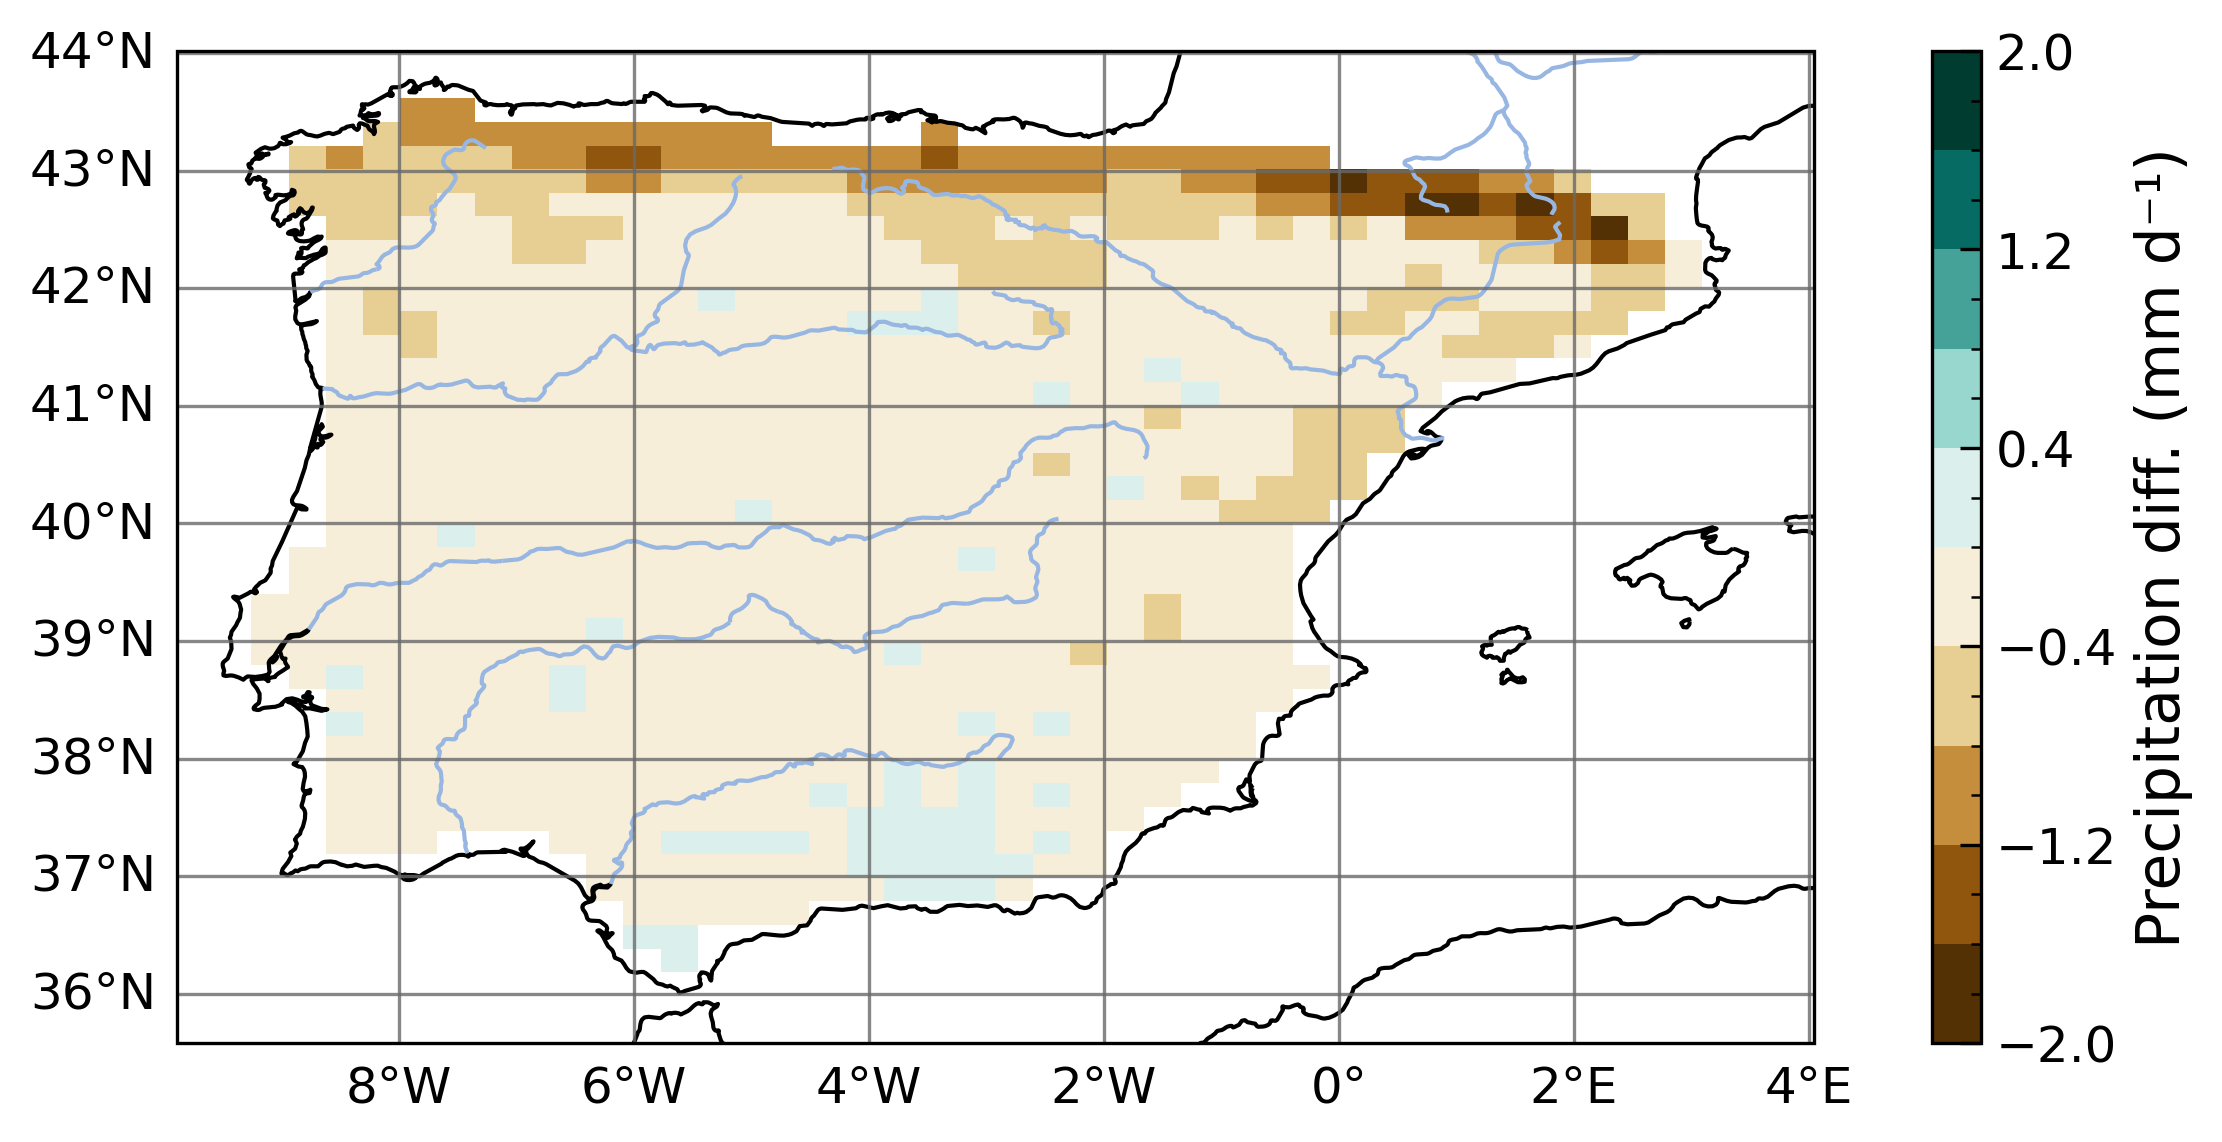
\includegraphics[width=\textwidth]{images/chap4/future/diffmap_JJA_precip_presfut.png}
%         \end{subfigure} &
%         %evap
%         \begin{subfigure}[b]{0.5\textwidth}
%             \caption{}
%             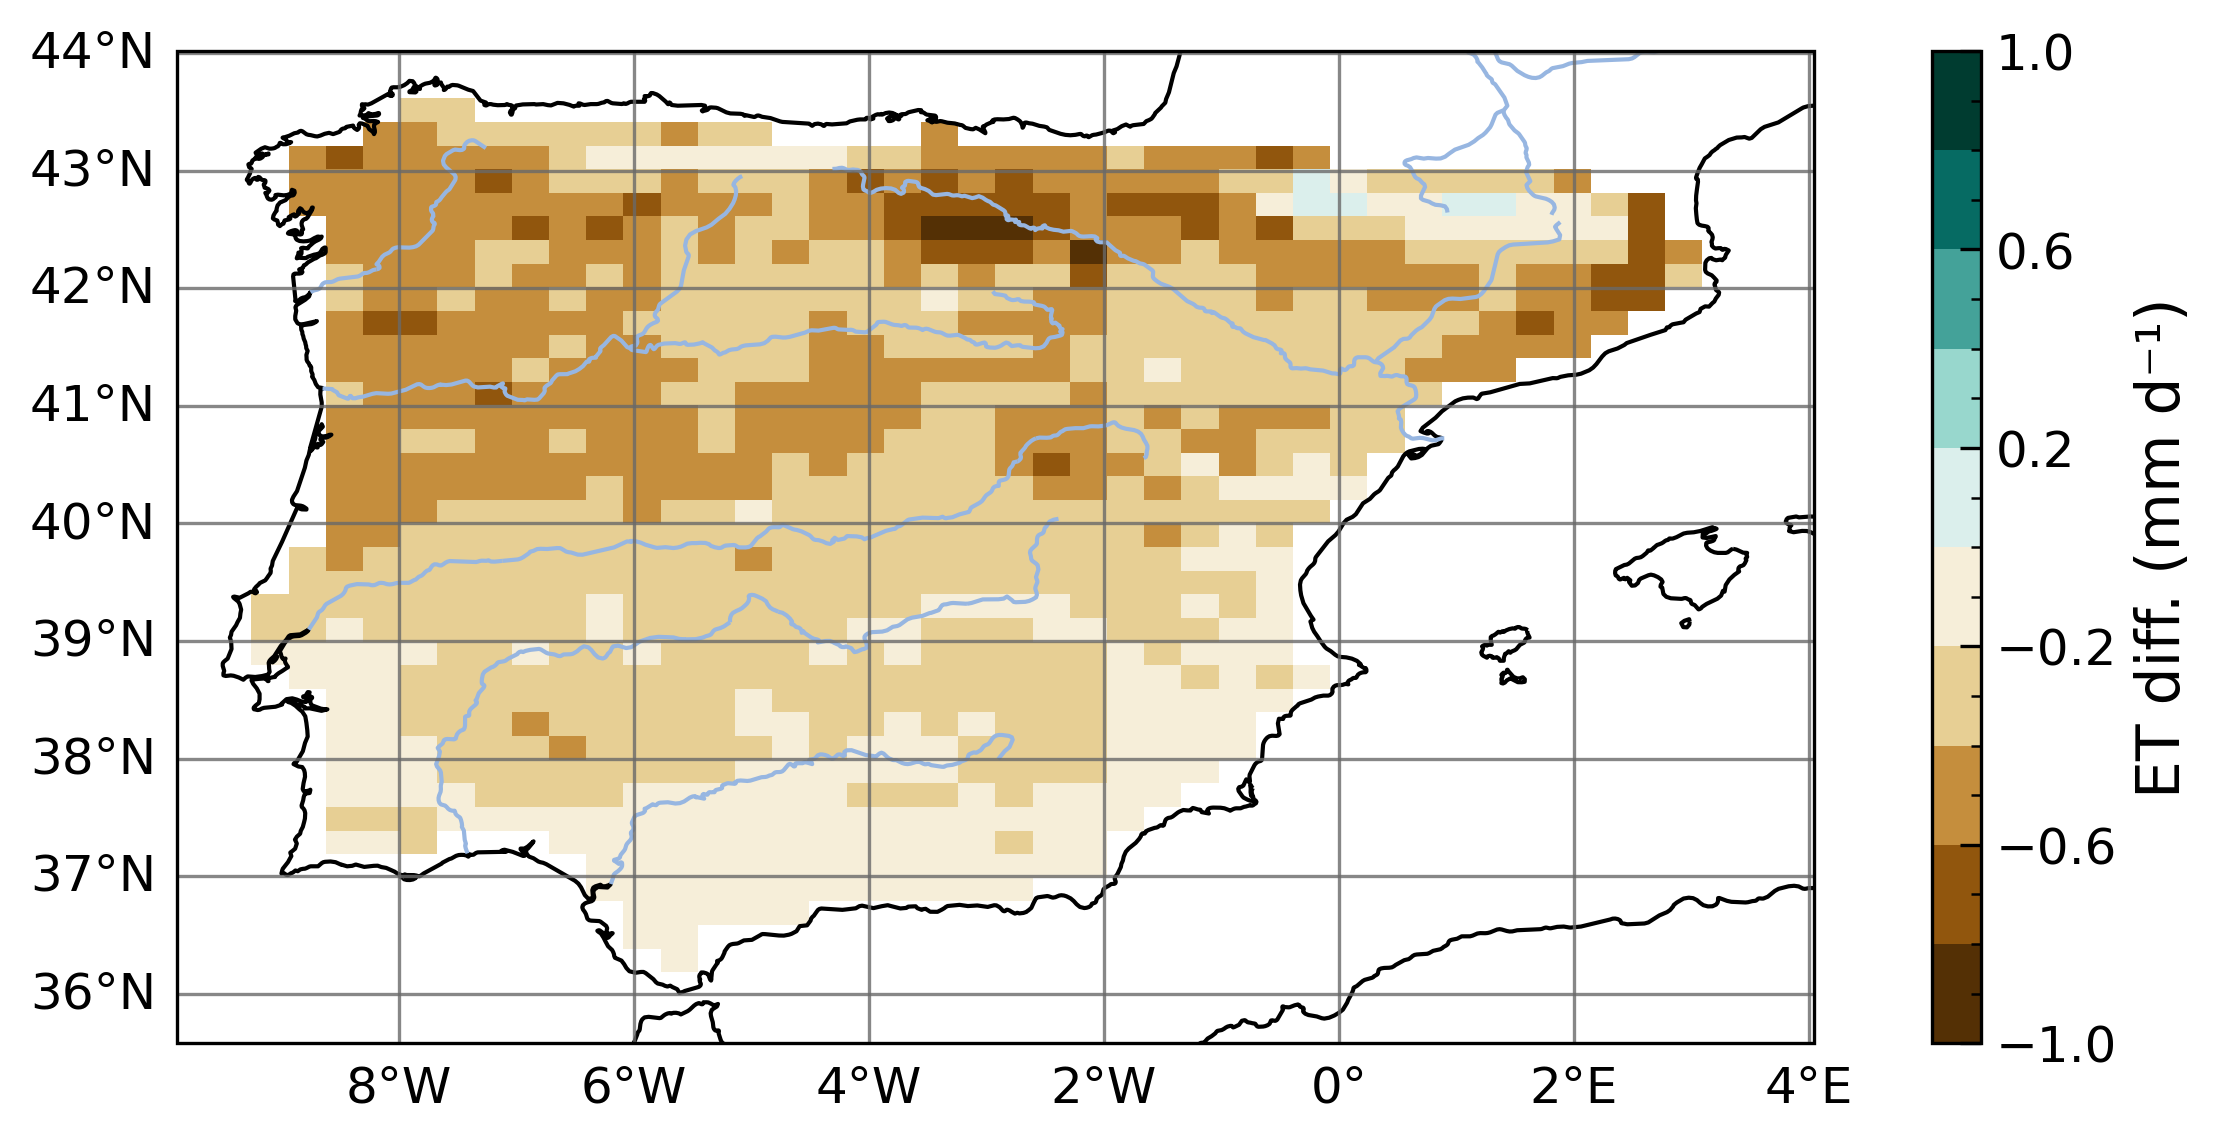
\includegraphics[width=\textwidth]{images/chap4/future/diffmap_JJA_evap_presfut.png}
%         \end{subfigure} \\

%         %t2m
%         \begin{subfigure}[b]{0.5\textwidth}
%             \caption{}
%             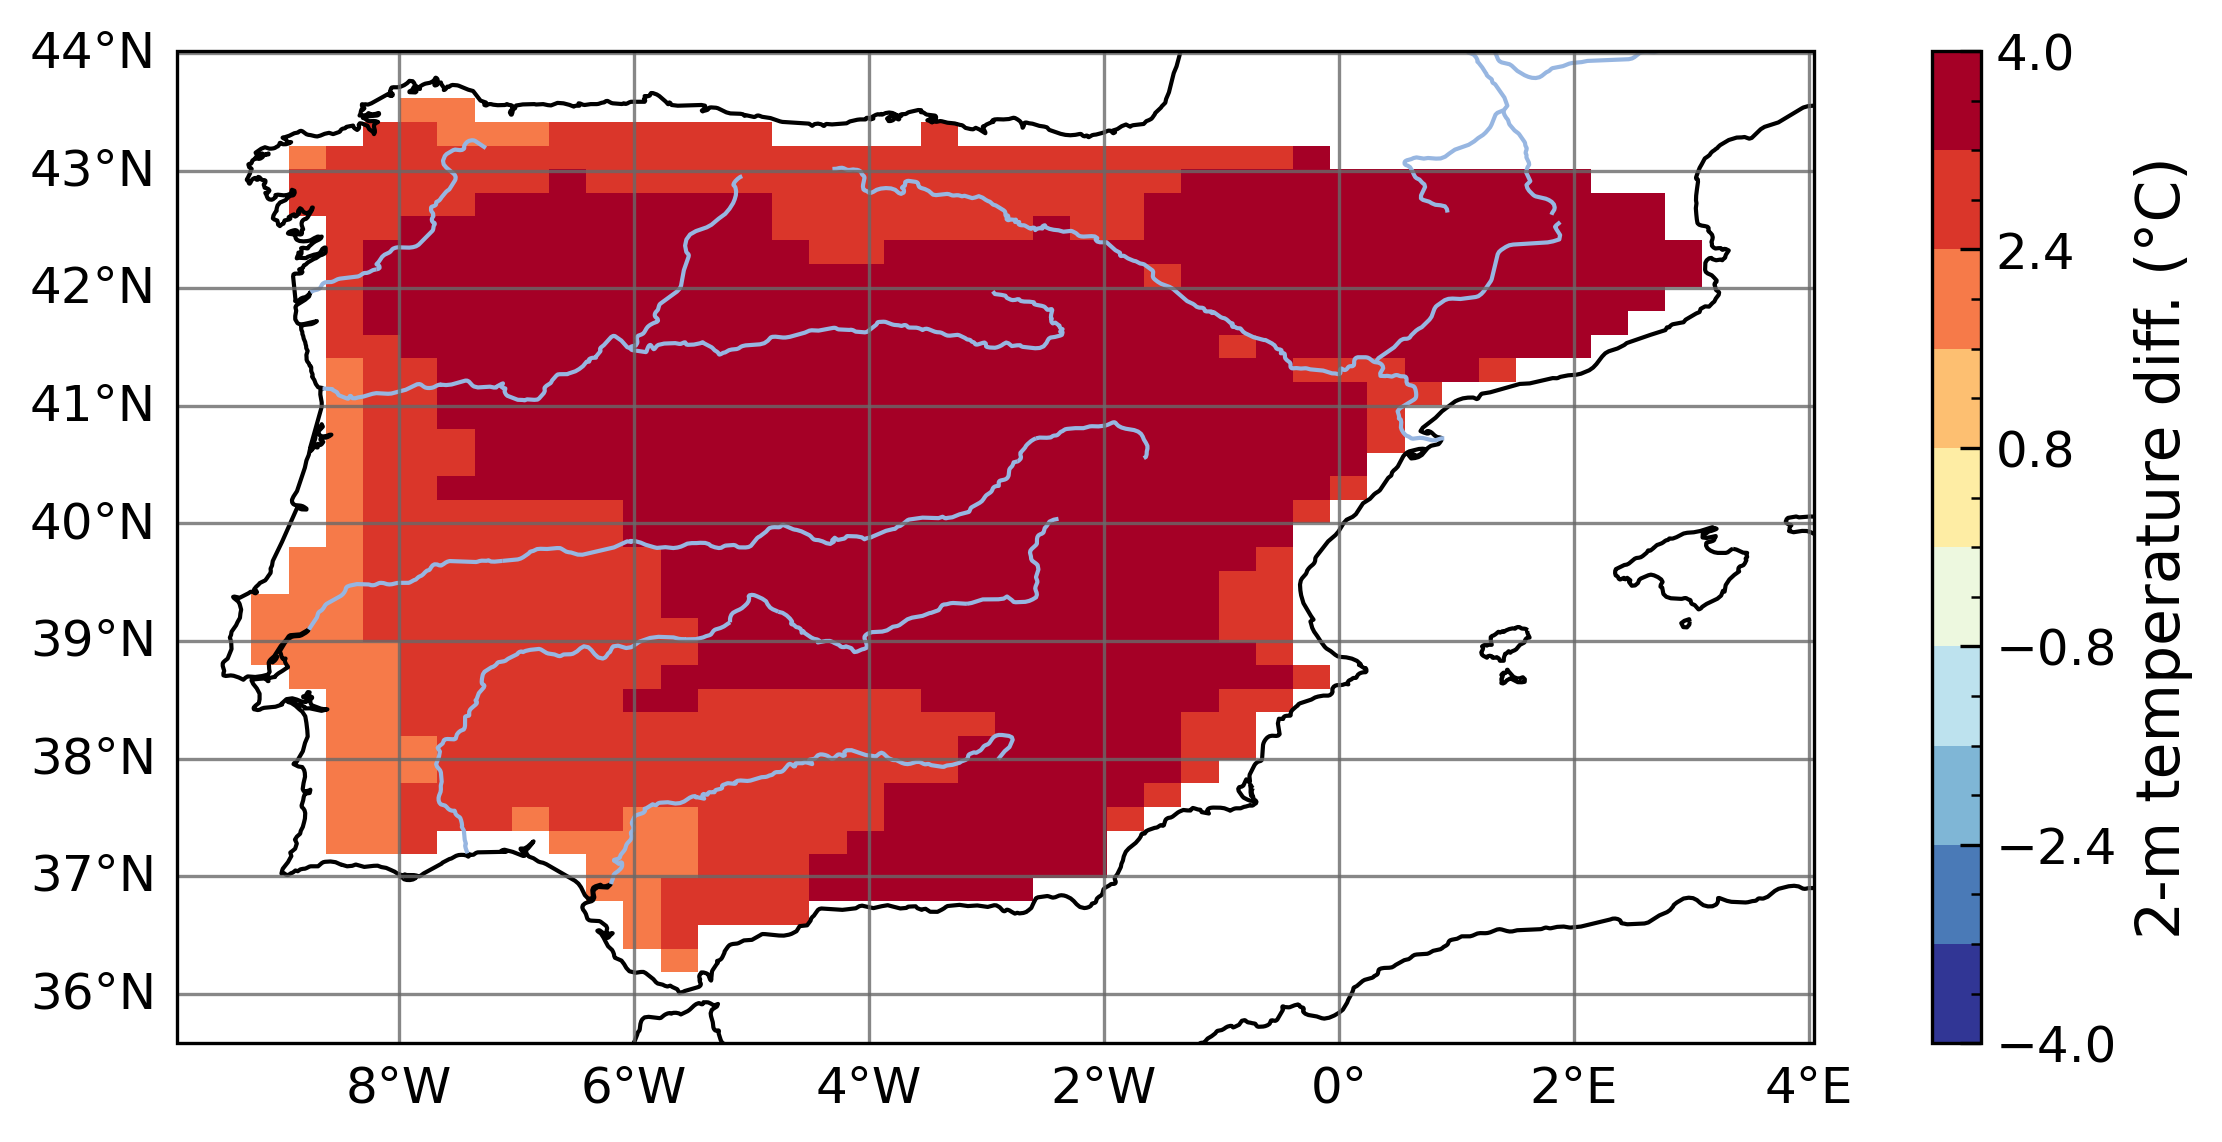
\includegraphics[width=\textwidth]{images/chap4/future/diffmap_JJA_t2m_presfut.png}
%         \end{subfigure} &
%         %fluxsens
%         \begin{subfigure}[b]{0.5\textwidth}
%             \caption{}
%             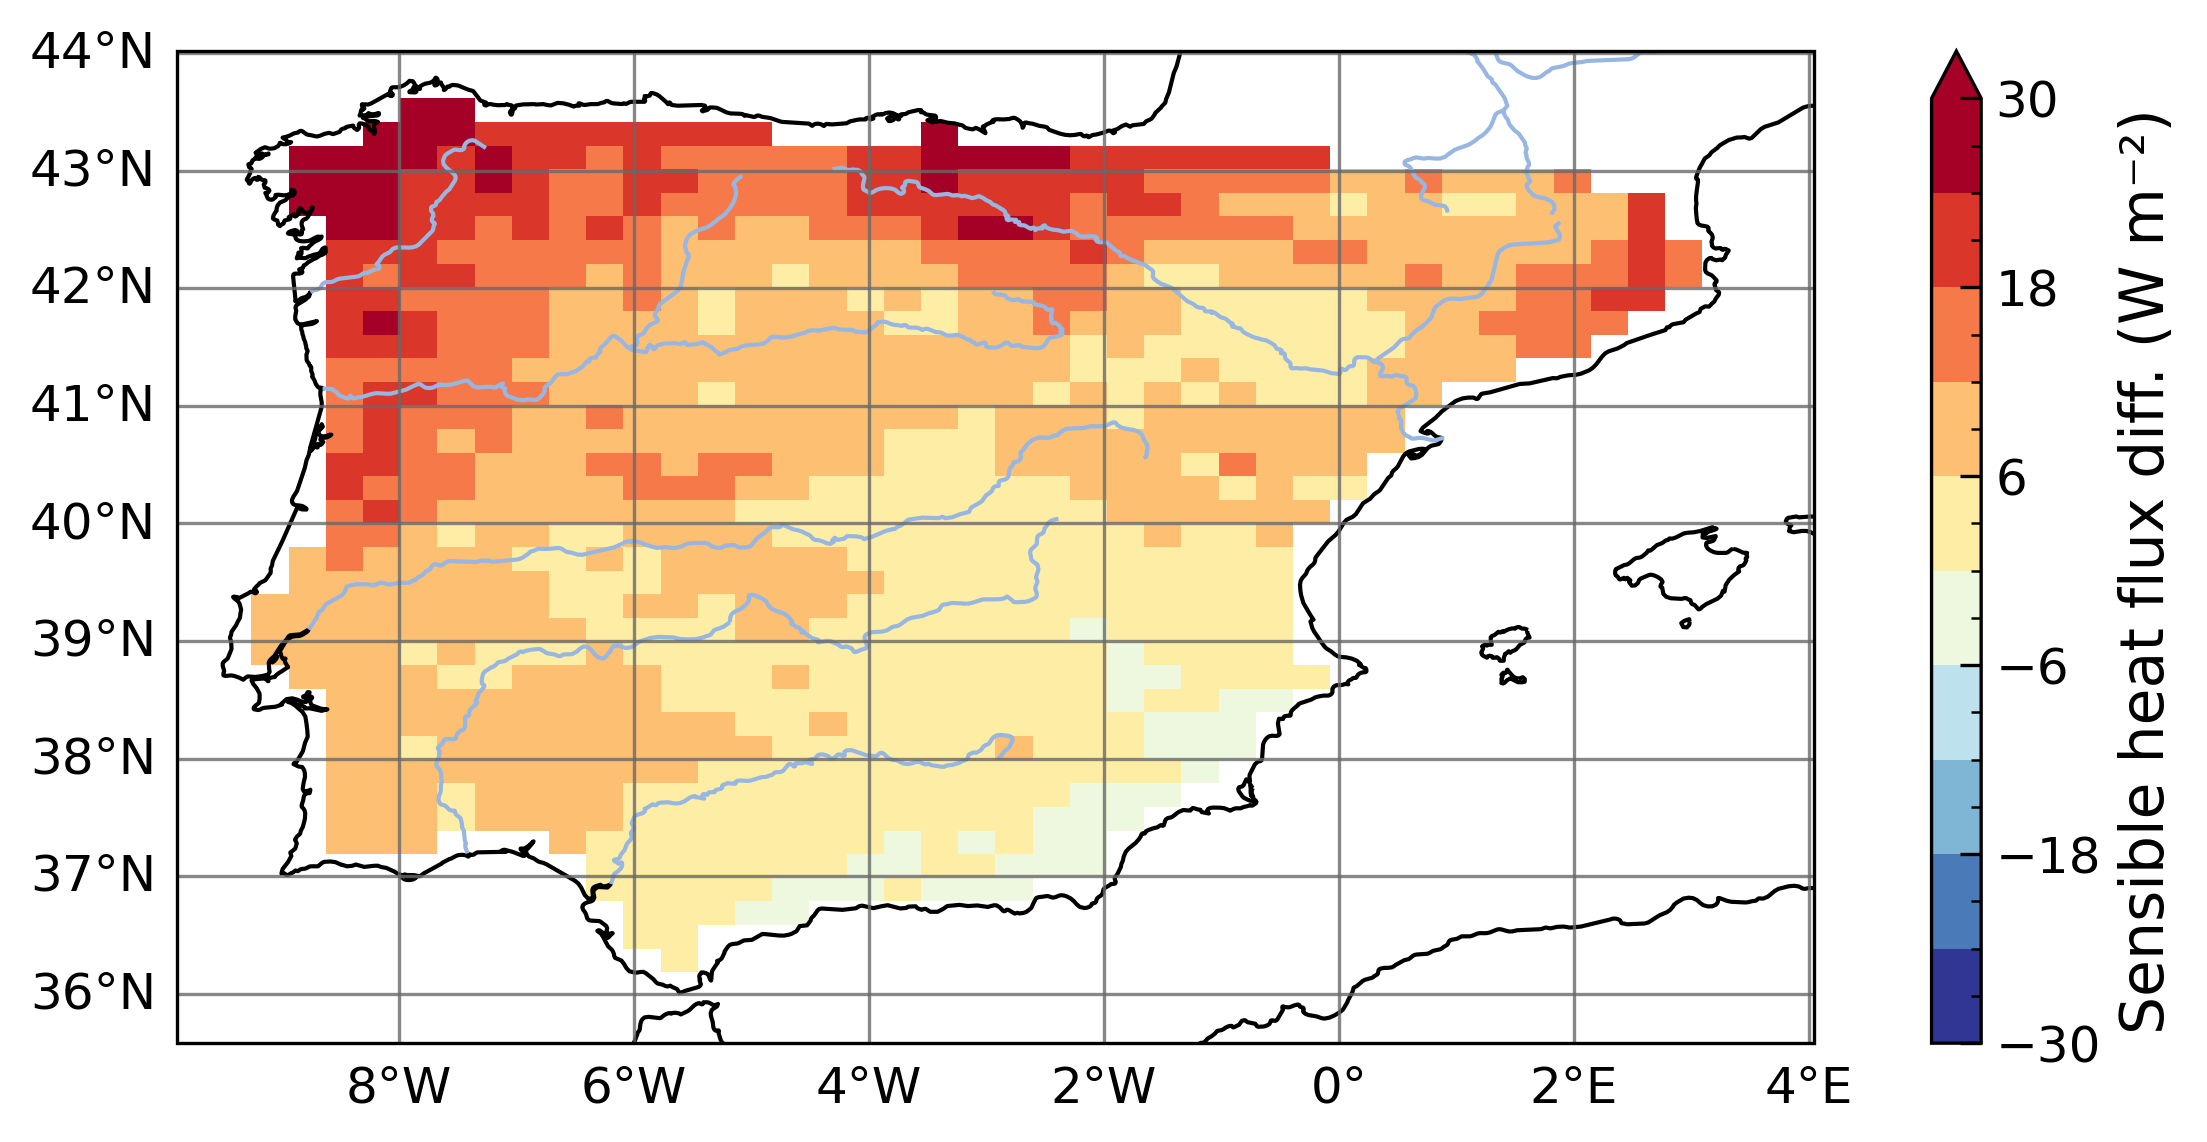
\includegraphics[width=\textwidth]{images/chap4/future/diffmap_JJA_fluxsens_presfut.png}
%         \end{subfigure} \\

%         %q2m
%         \begin{subfigure}[b]{0.5\textwidth}
%             \caption{}
%             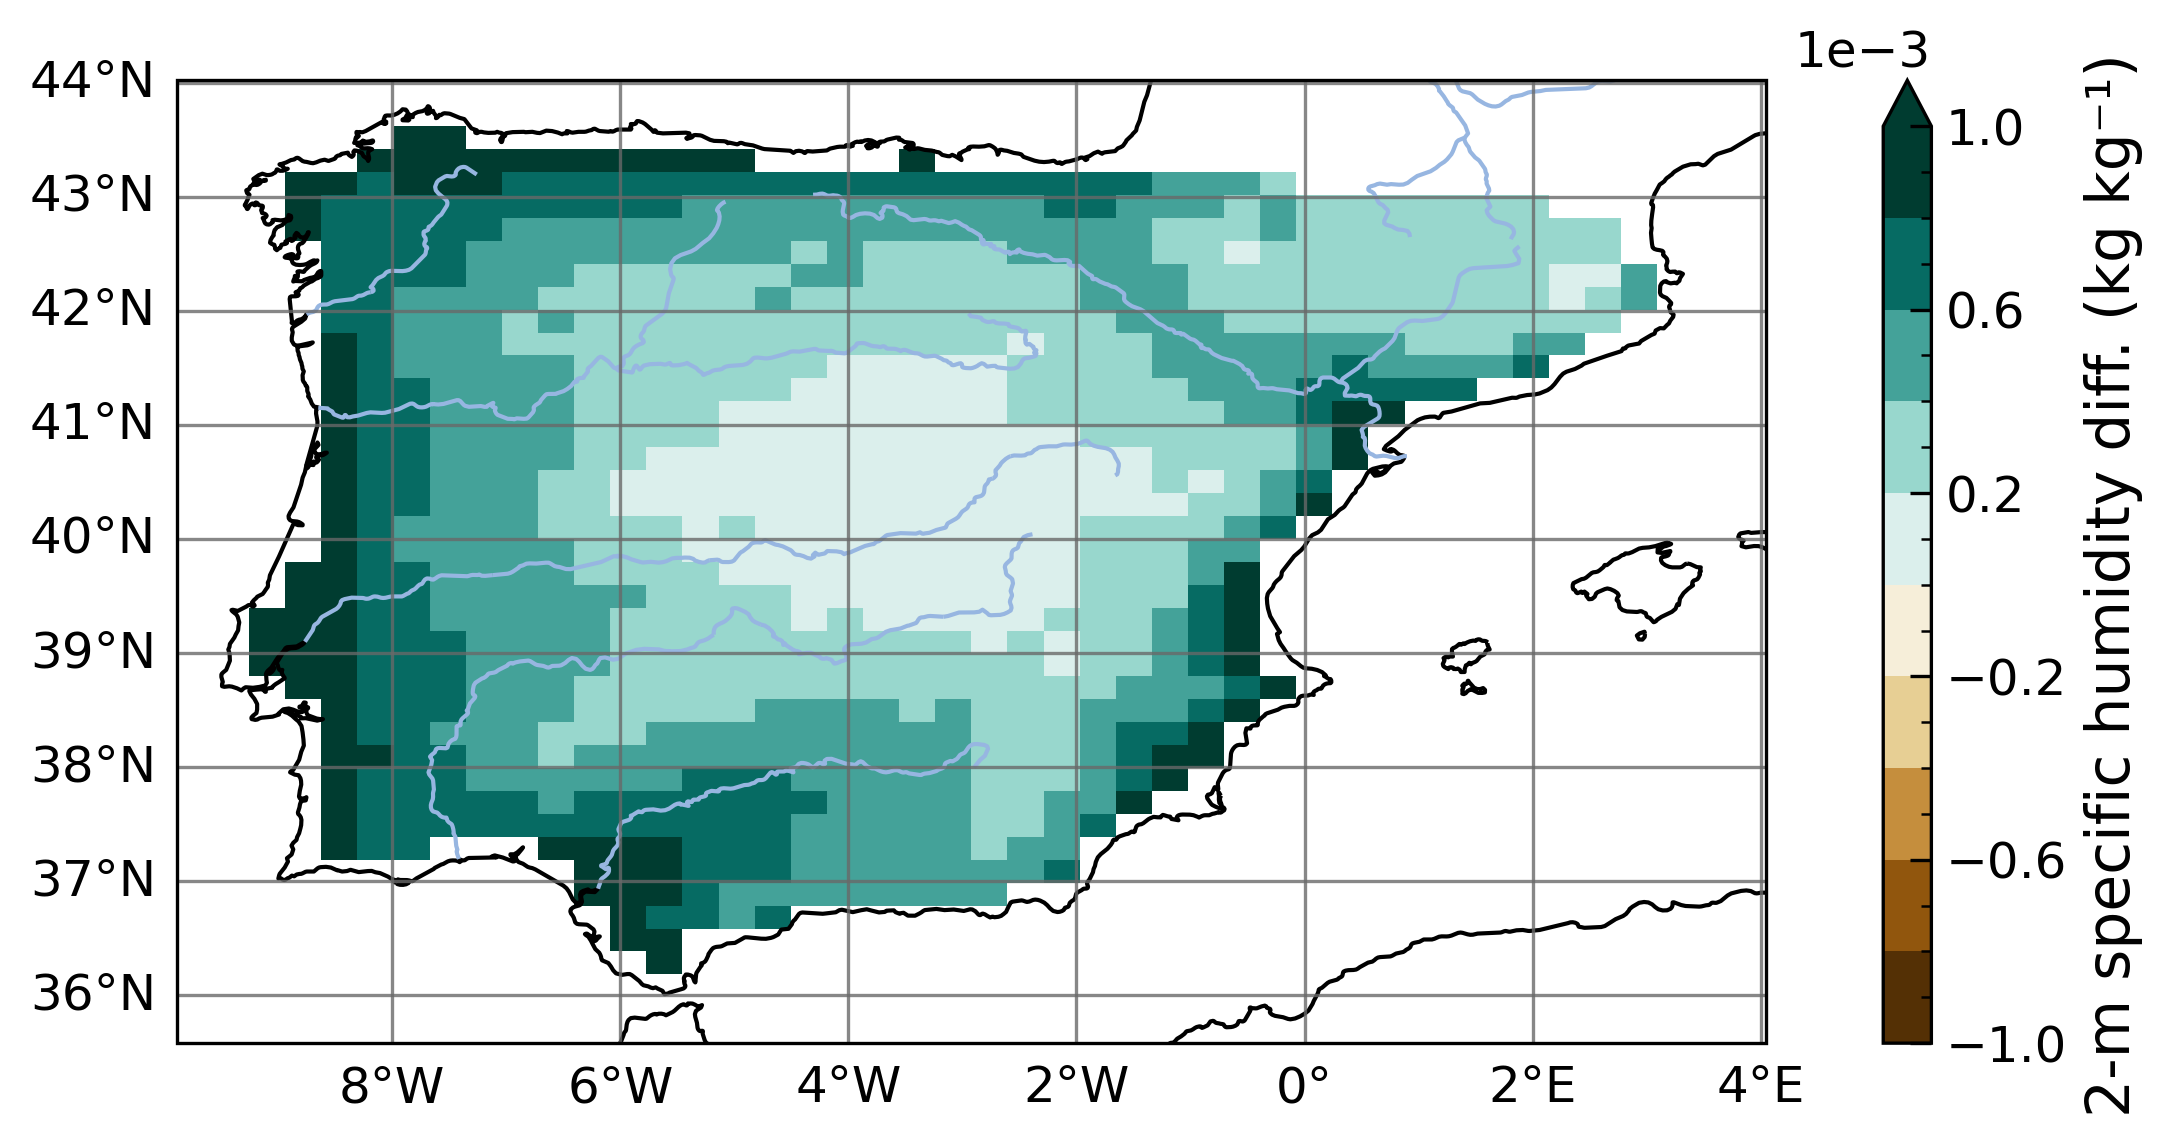
\includegraphics[width=\textwidth]{images/chap4/future/diffmap_JJA_q2m_presfut.png}
%         \end{subfigure} &
%         %rh2m
%         \begin{subfigure}[b]{0.5\textwidth}
%             \caption{}
%             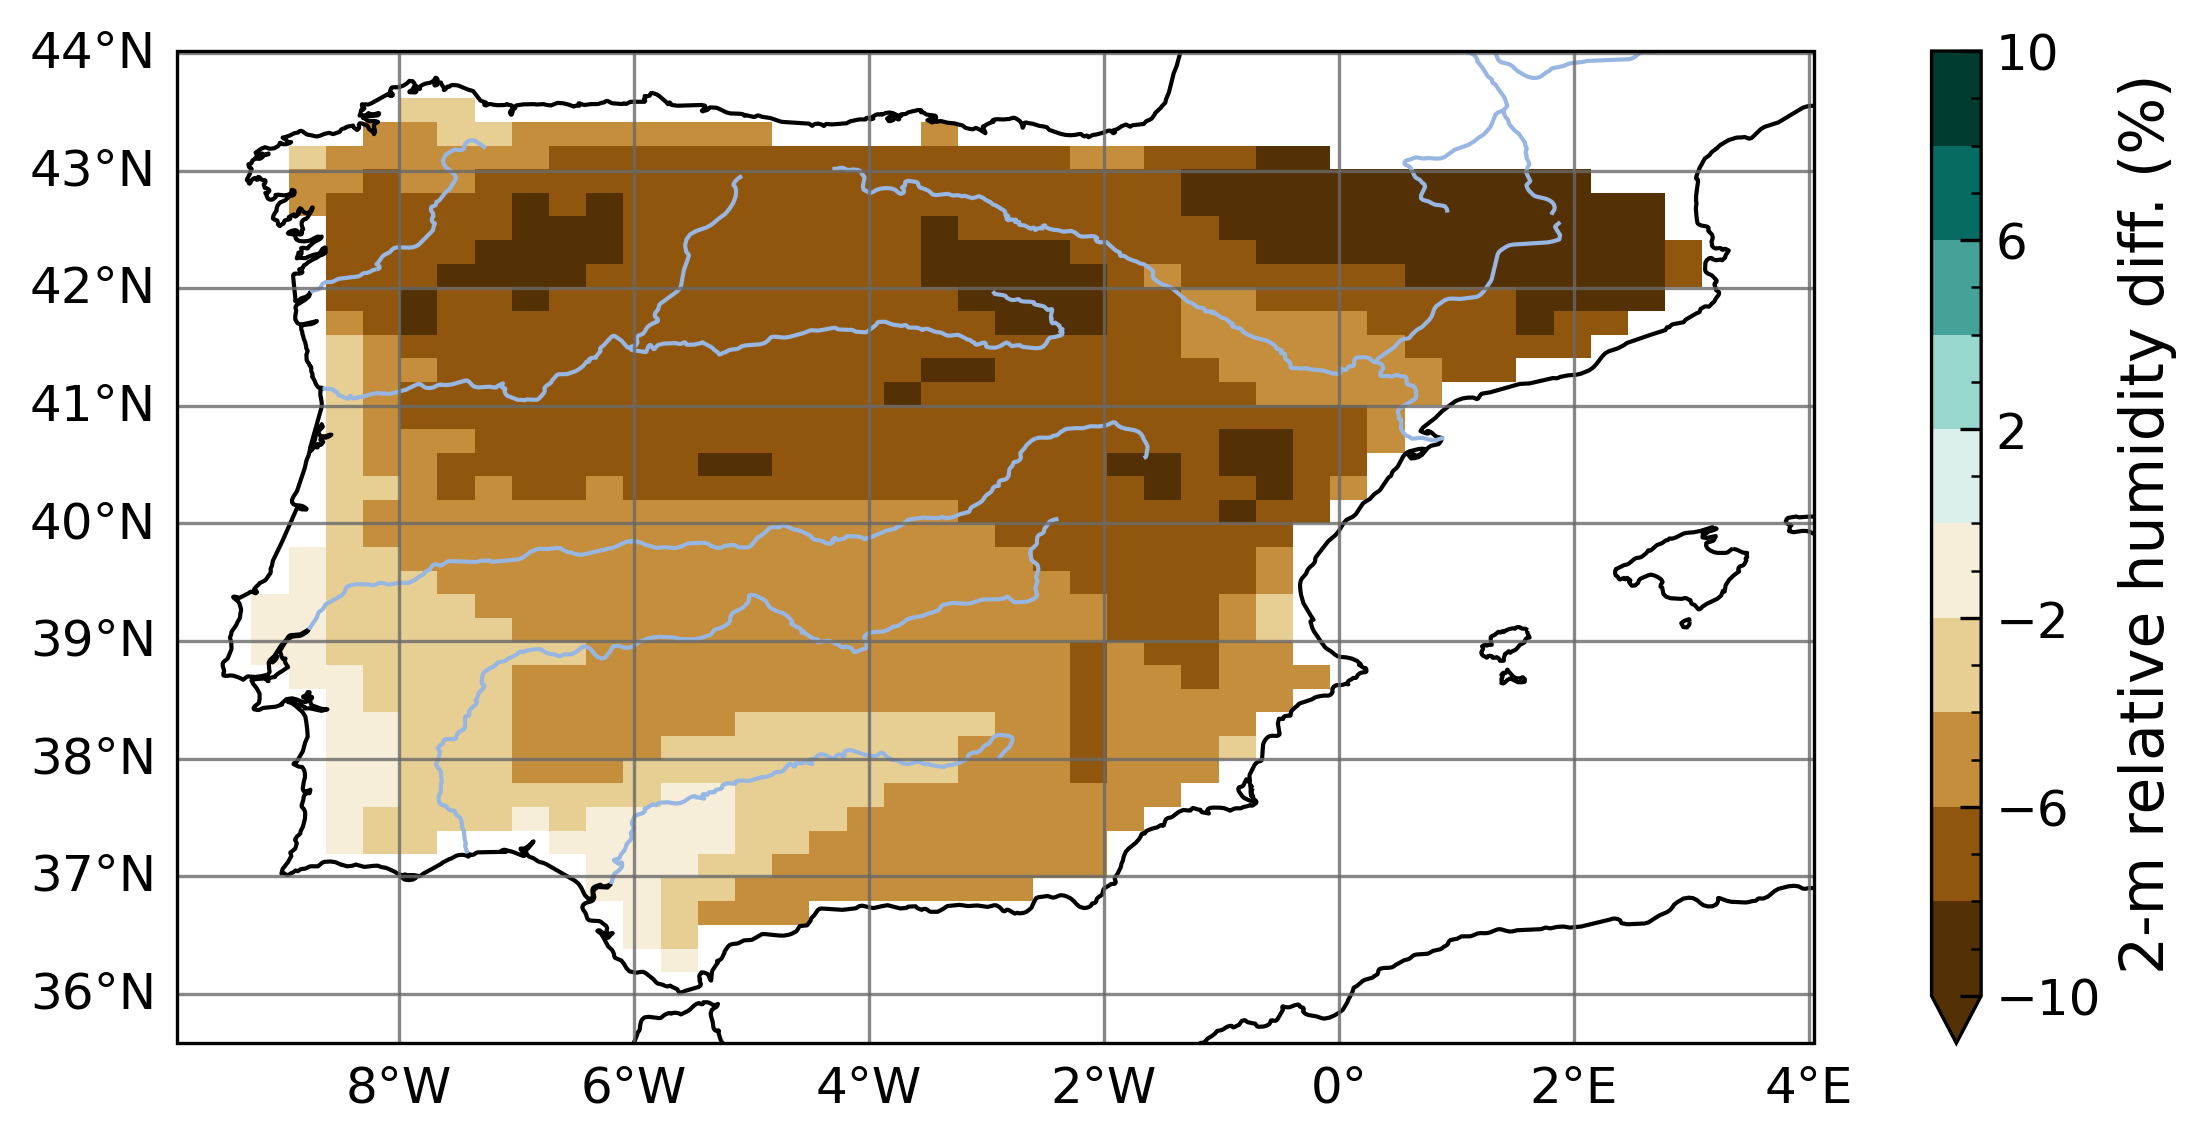
\includegraphics[width=\textwidth]{images/chap4/future/diffmap_JJA_rh2m_presfut.png}
%         \end{subfigure} \\

%         %pblh
%         \begin{subfigure}[b]{0.5\textwidth}
%             \caption{}
%             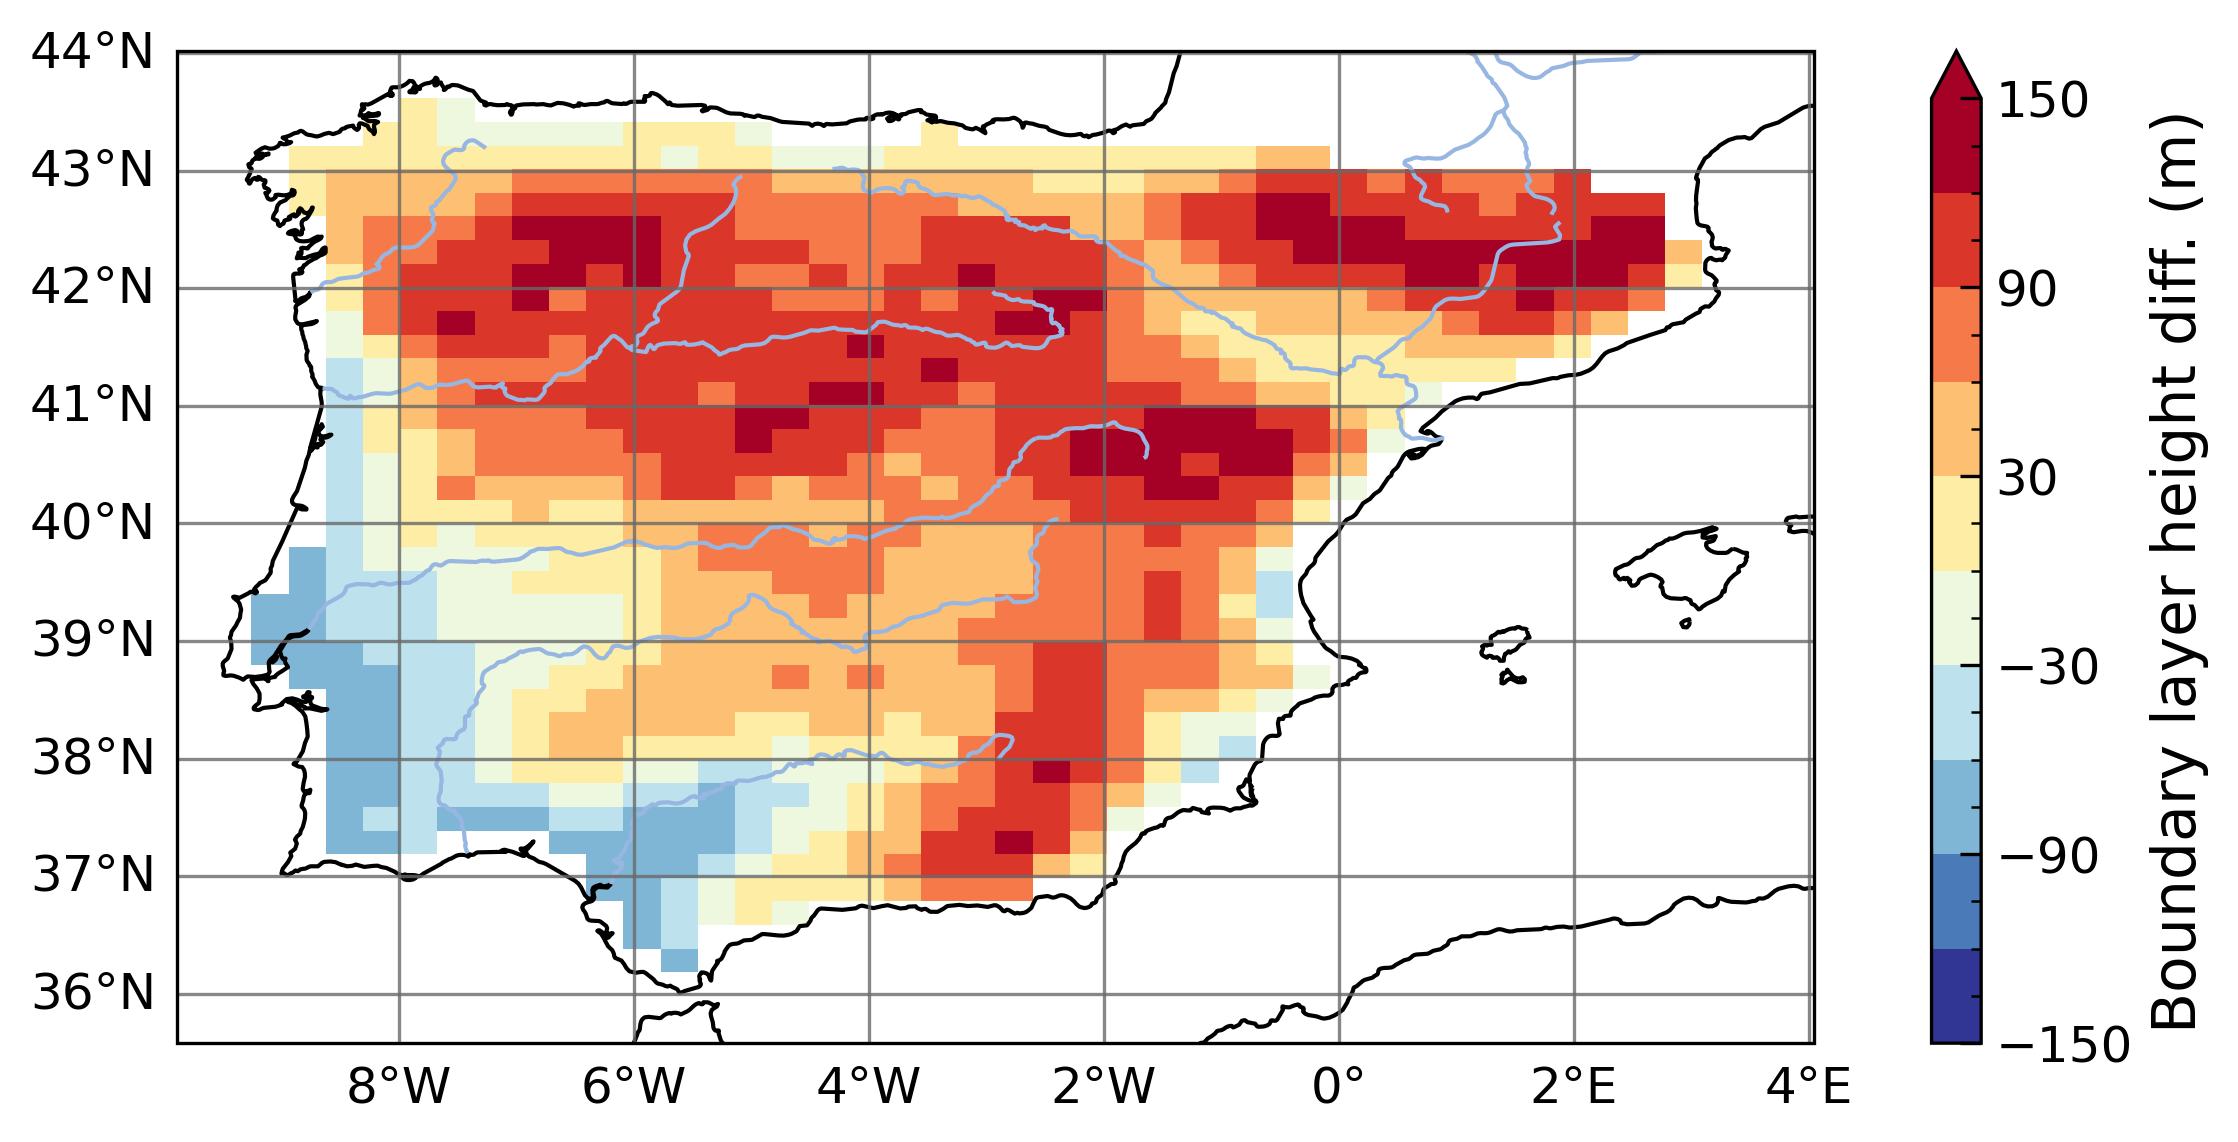
\includegraphics[width=\textwidth]{images/chap4/future/diffmap_JJA_s_pblh_presfut.png}
%         \end{subfigure} &
%         %lcl
%         \begin{subfigure}[b]{0.5\textwidth}
%             \caption{}
%             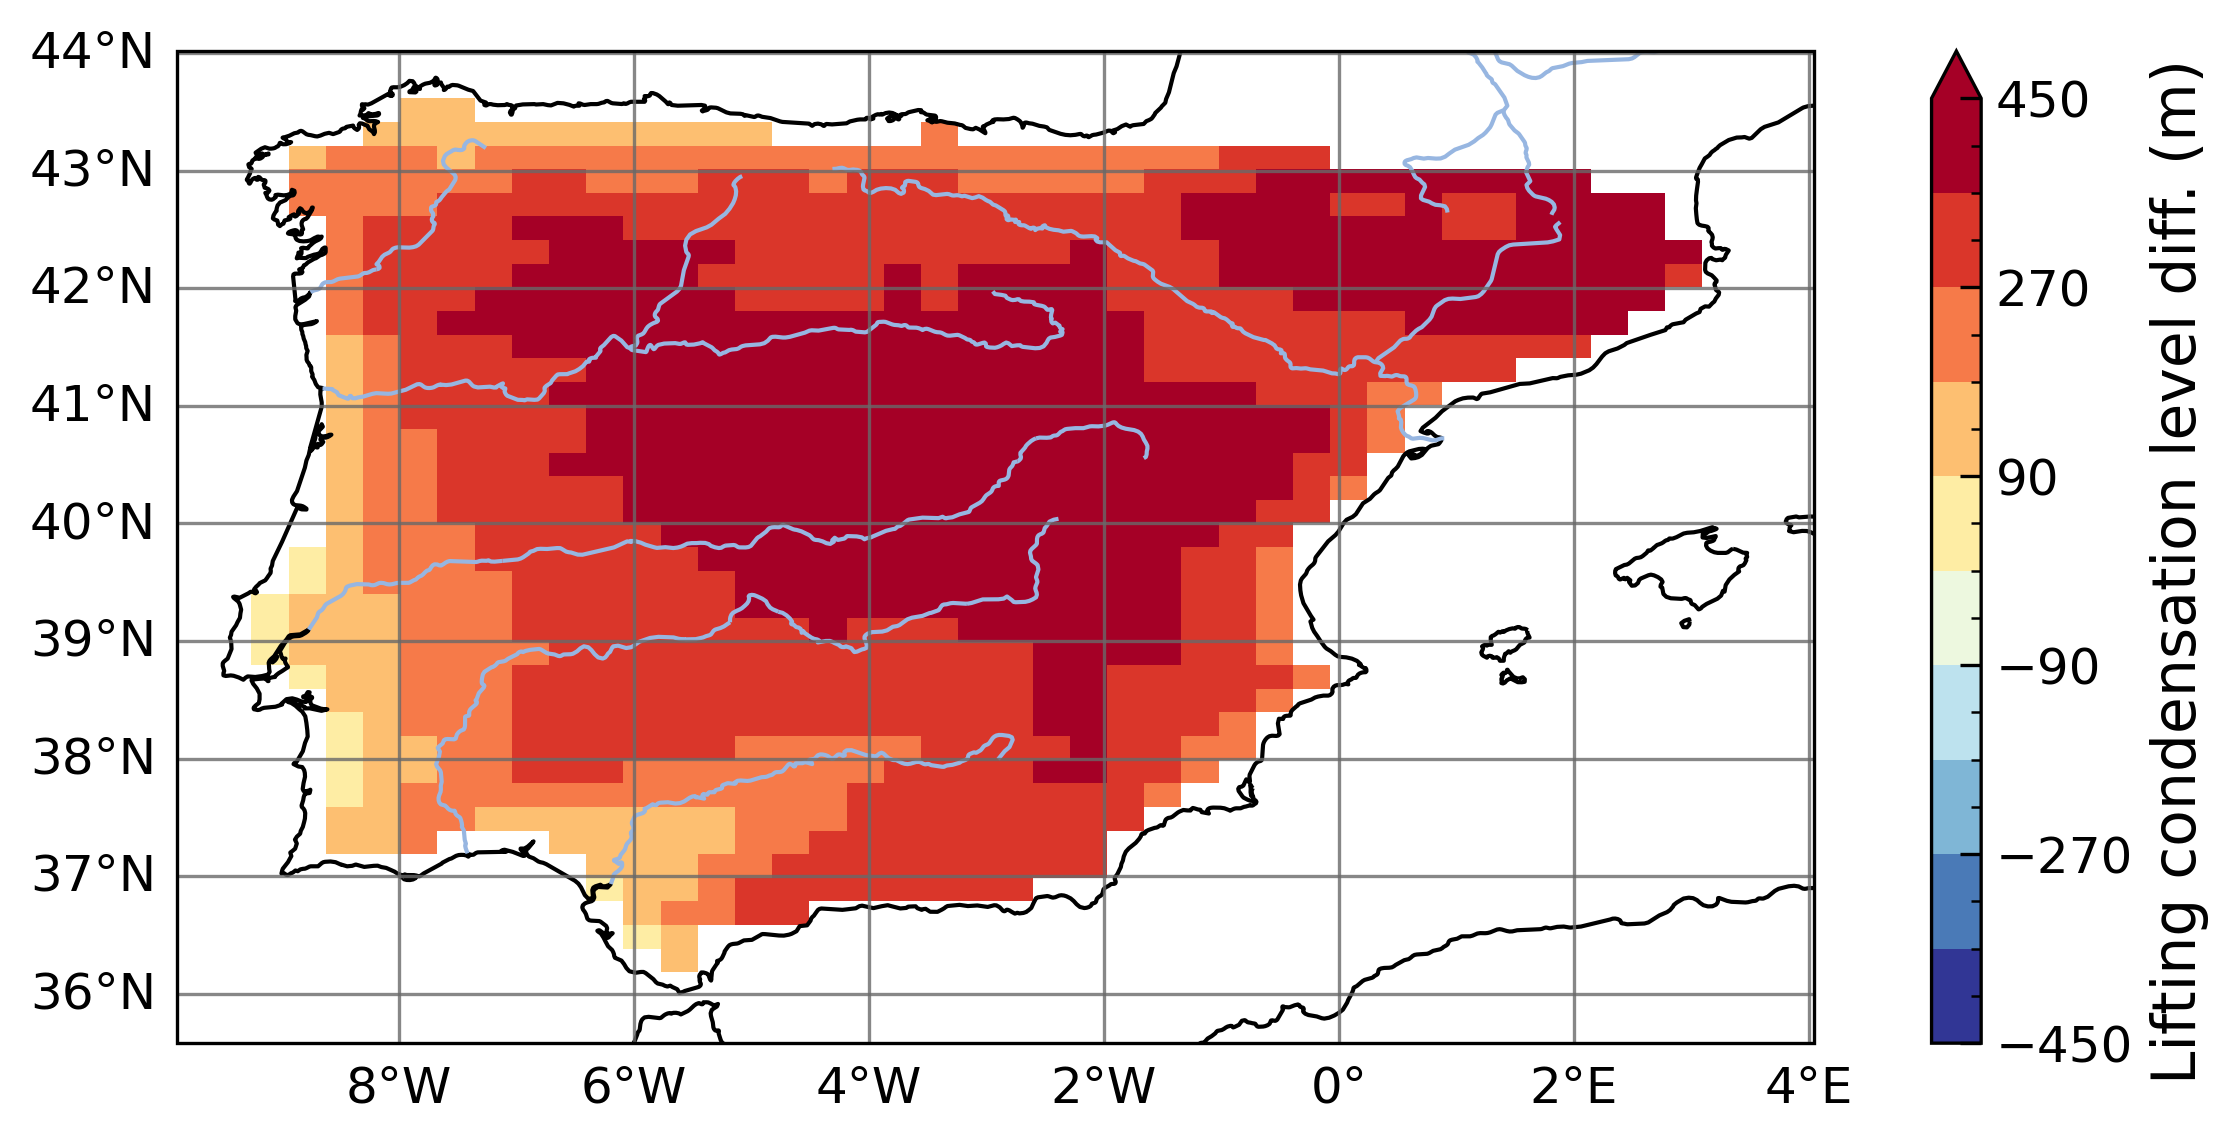
\includegraphics[width=\textwidth]{images/chap4/future/diffmap_JJA_s_lcl_presfut.png}
%         \end{subfigure} \\
%     \end{tabular}
%     \caption{JJA difference (\futnoirr - \presnoirr)}
%     \label{fig:diffmaps_JJA_present_future}
% \end{figure}

%figure : relative diff maps annual (noirr, pres - future)
\begin{figure}[htbp]
    \centering
    \begin{tabular}{cc}
        %precip
        \begin{subfigure}[b]{0.5\textwidth}
            \caption{}
            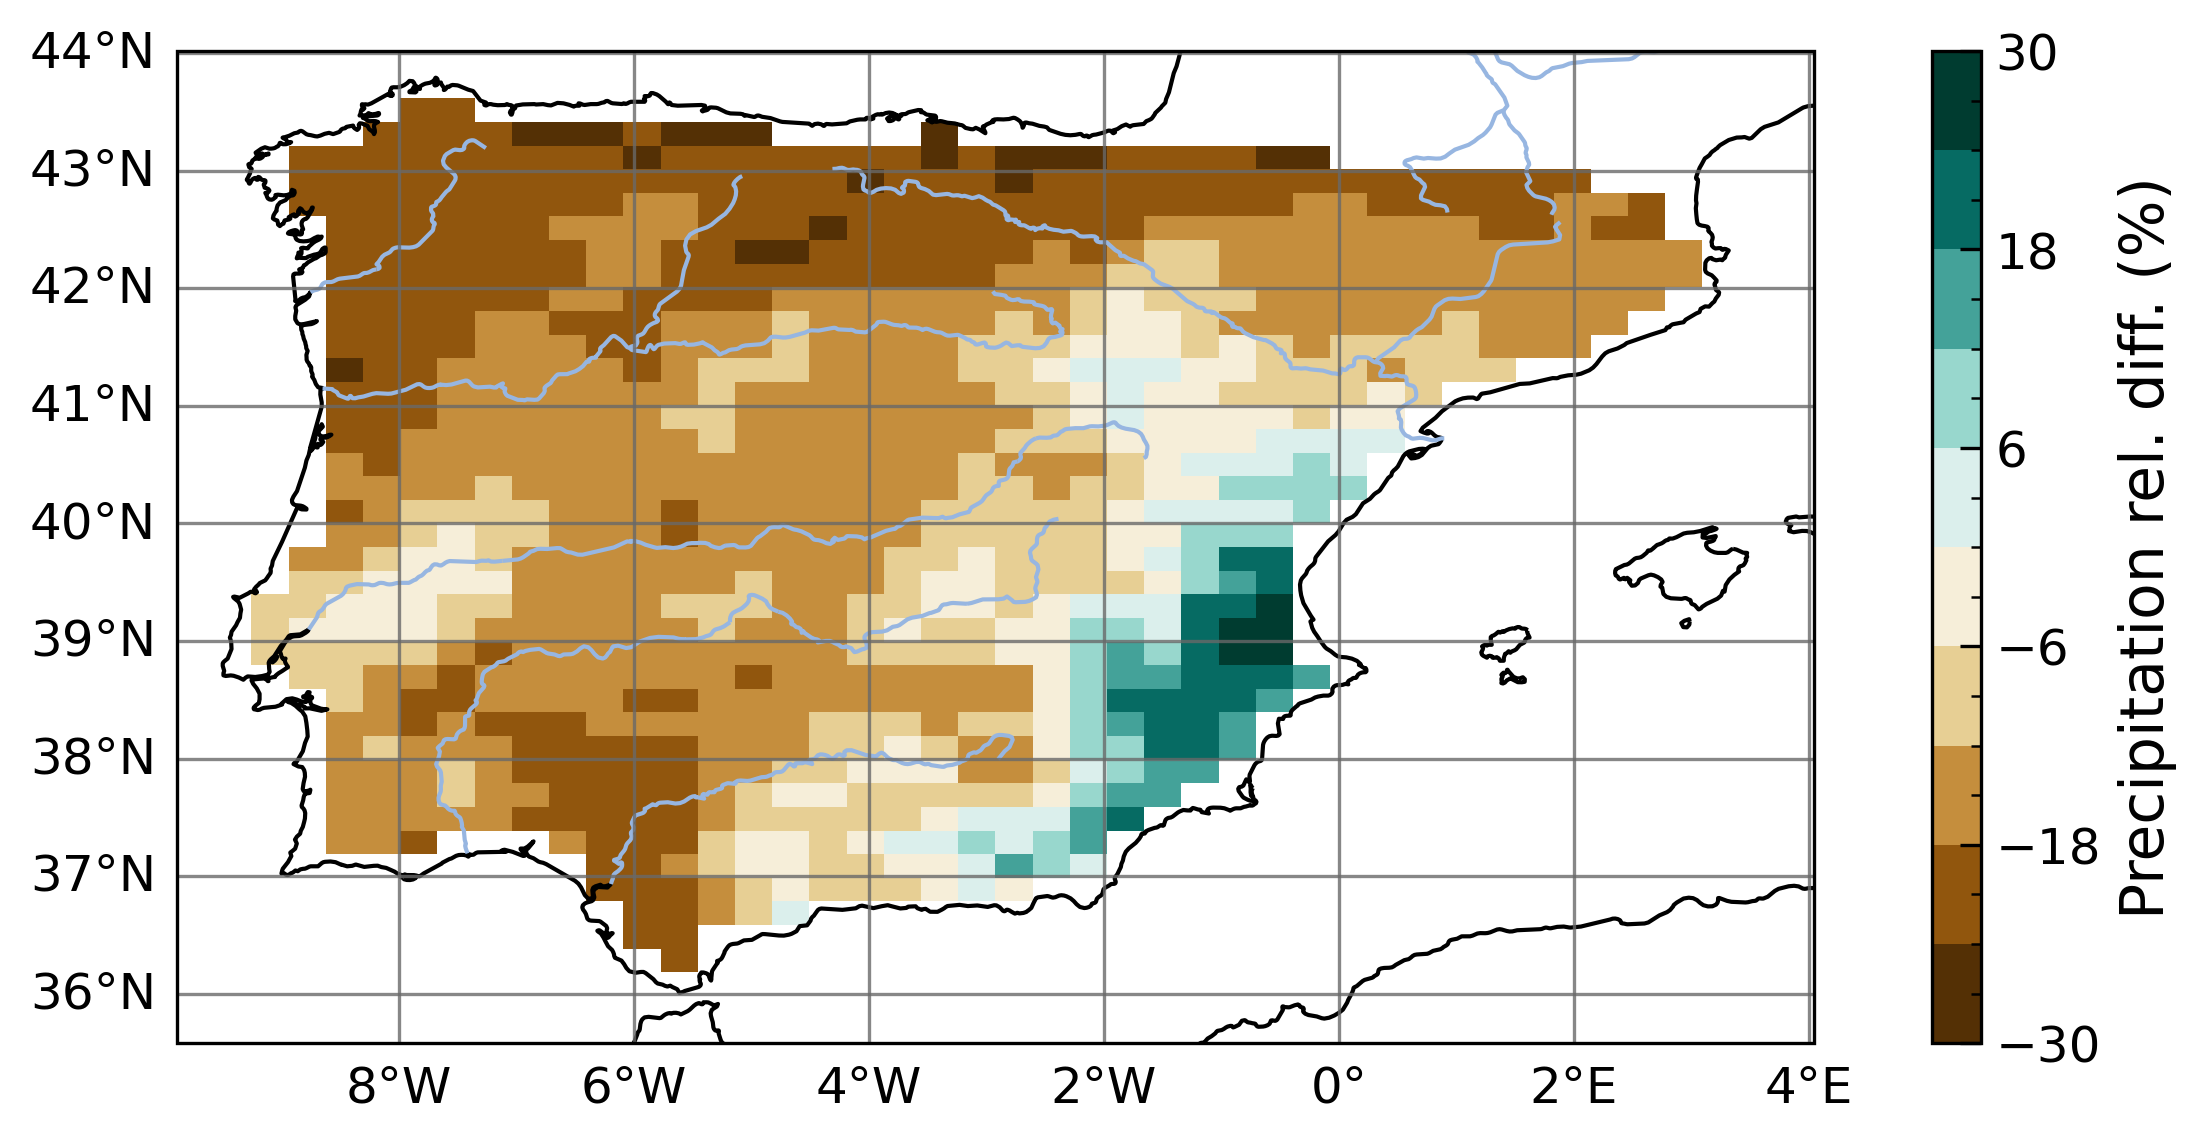
\includegraphics[width=\textwidth]{images/chap4/future/reldiffmap_precip_presfut.png}
        \end{subfigure} &
        %evap
        \begin{subfigure}[b]{0.5\textwidth}
            \caption{}
            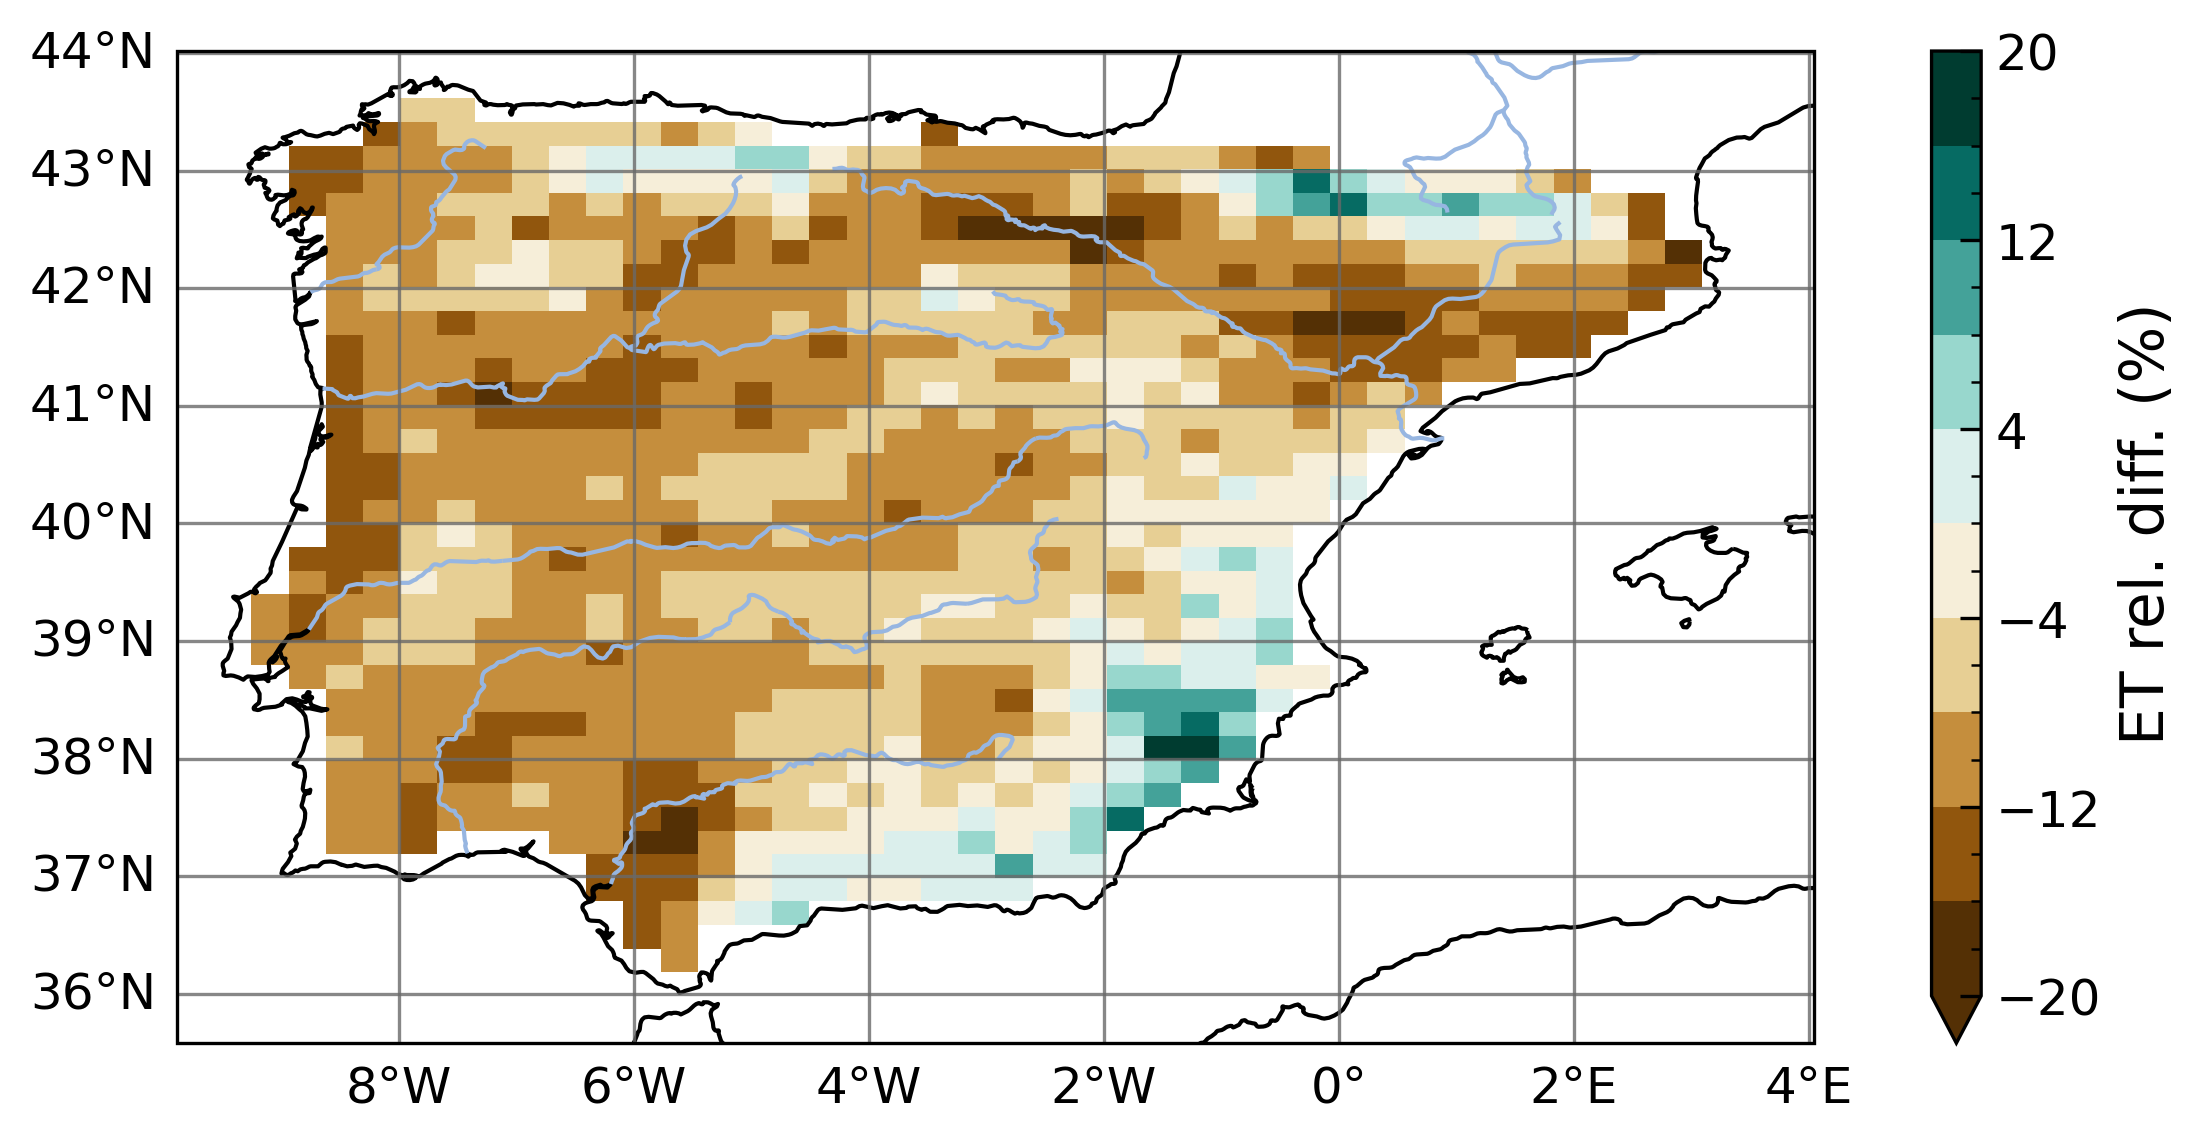
\includegraphics[width=\textwidth]{images/chap4/future/reldiffmap_evap_presfut.png}
        \end{subfigure} \\

        %t2m
        \begin{subfigure}[b]{0.5\textwidth}
            \caption{}
            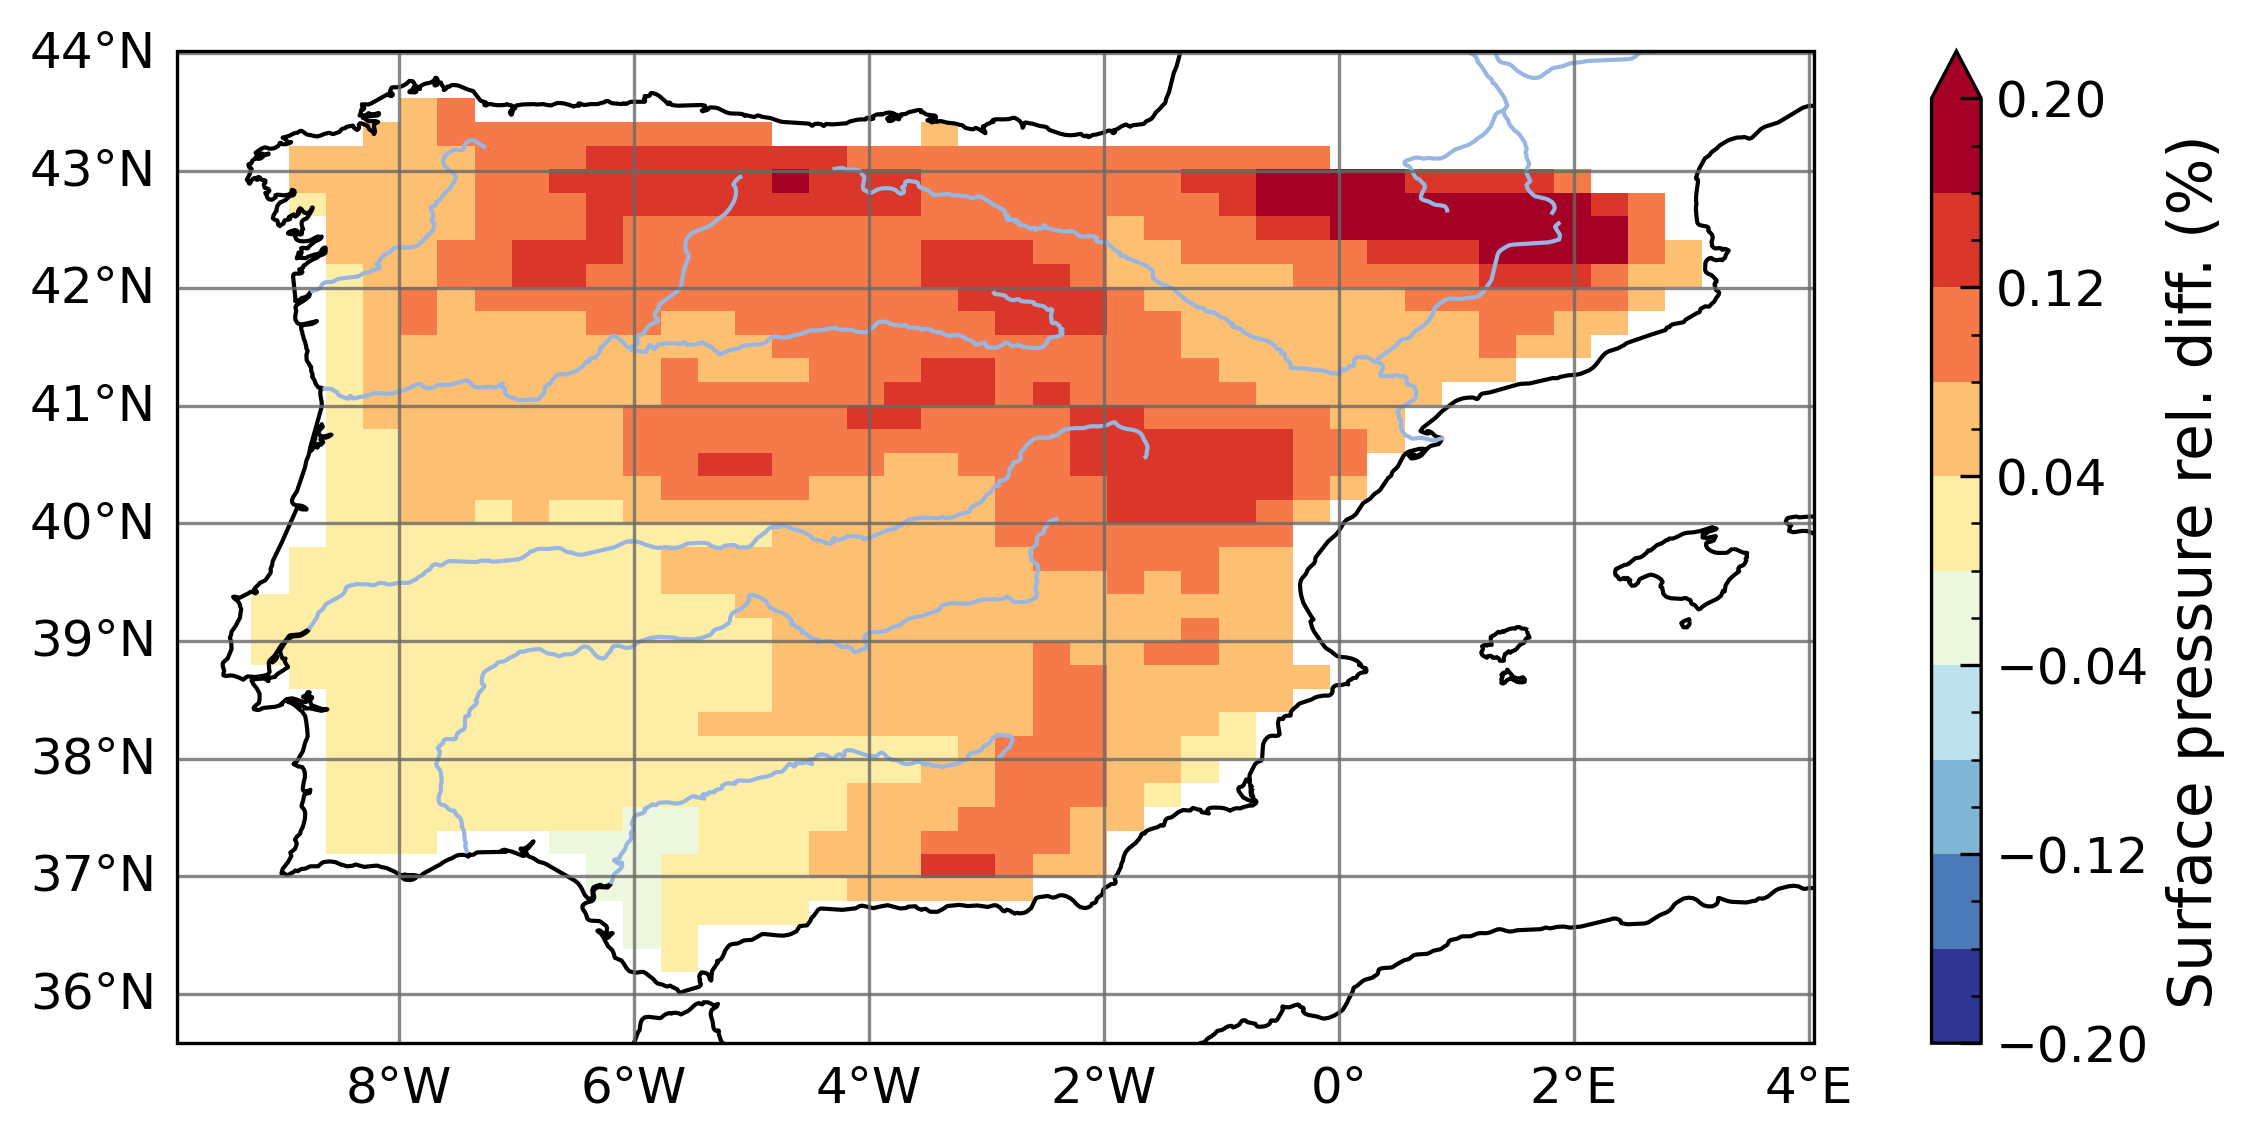
\includegraphics[width=\textwidth]{images/chap4/future/reldiffmap_psol_presfut.png}
        \end{subfigure} &
        %fluxsens
        \begin{subfigure}[b]{0.5\textwidth}
            \caption{}
            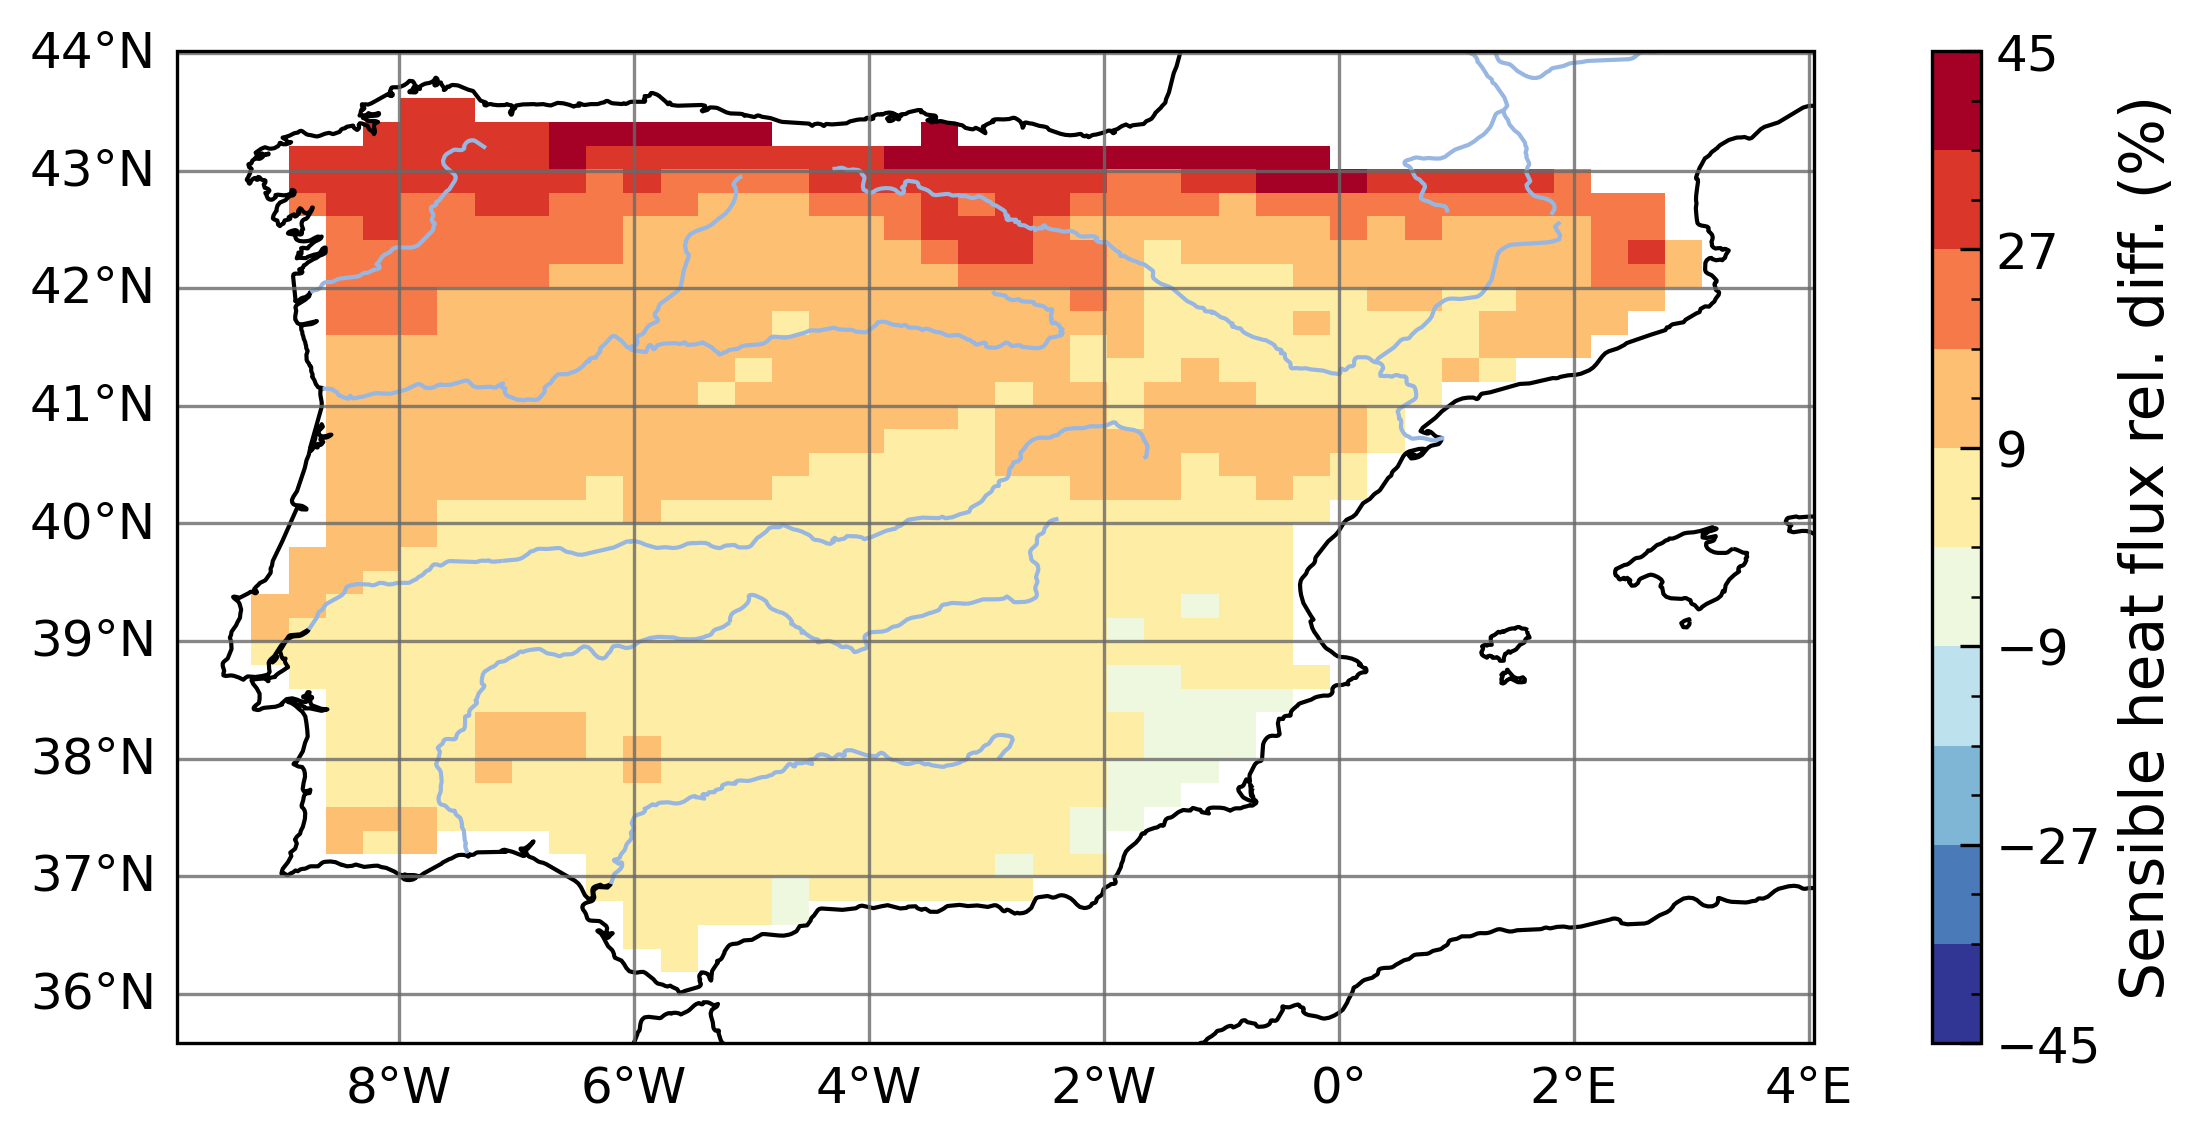
\includegraphics[width=\textwidth]{images/chap4/future/reldiffmap_fluxsens_presfut.png}
        \end{subfigure} \\

        %q2m
        \begin{subfigure}[b]{0.5\textwidth}
            \caption{}
            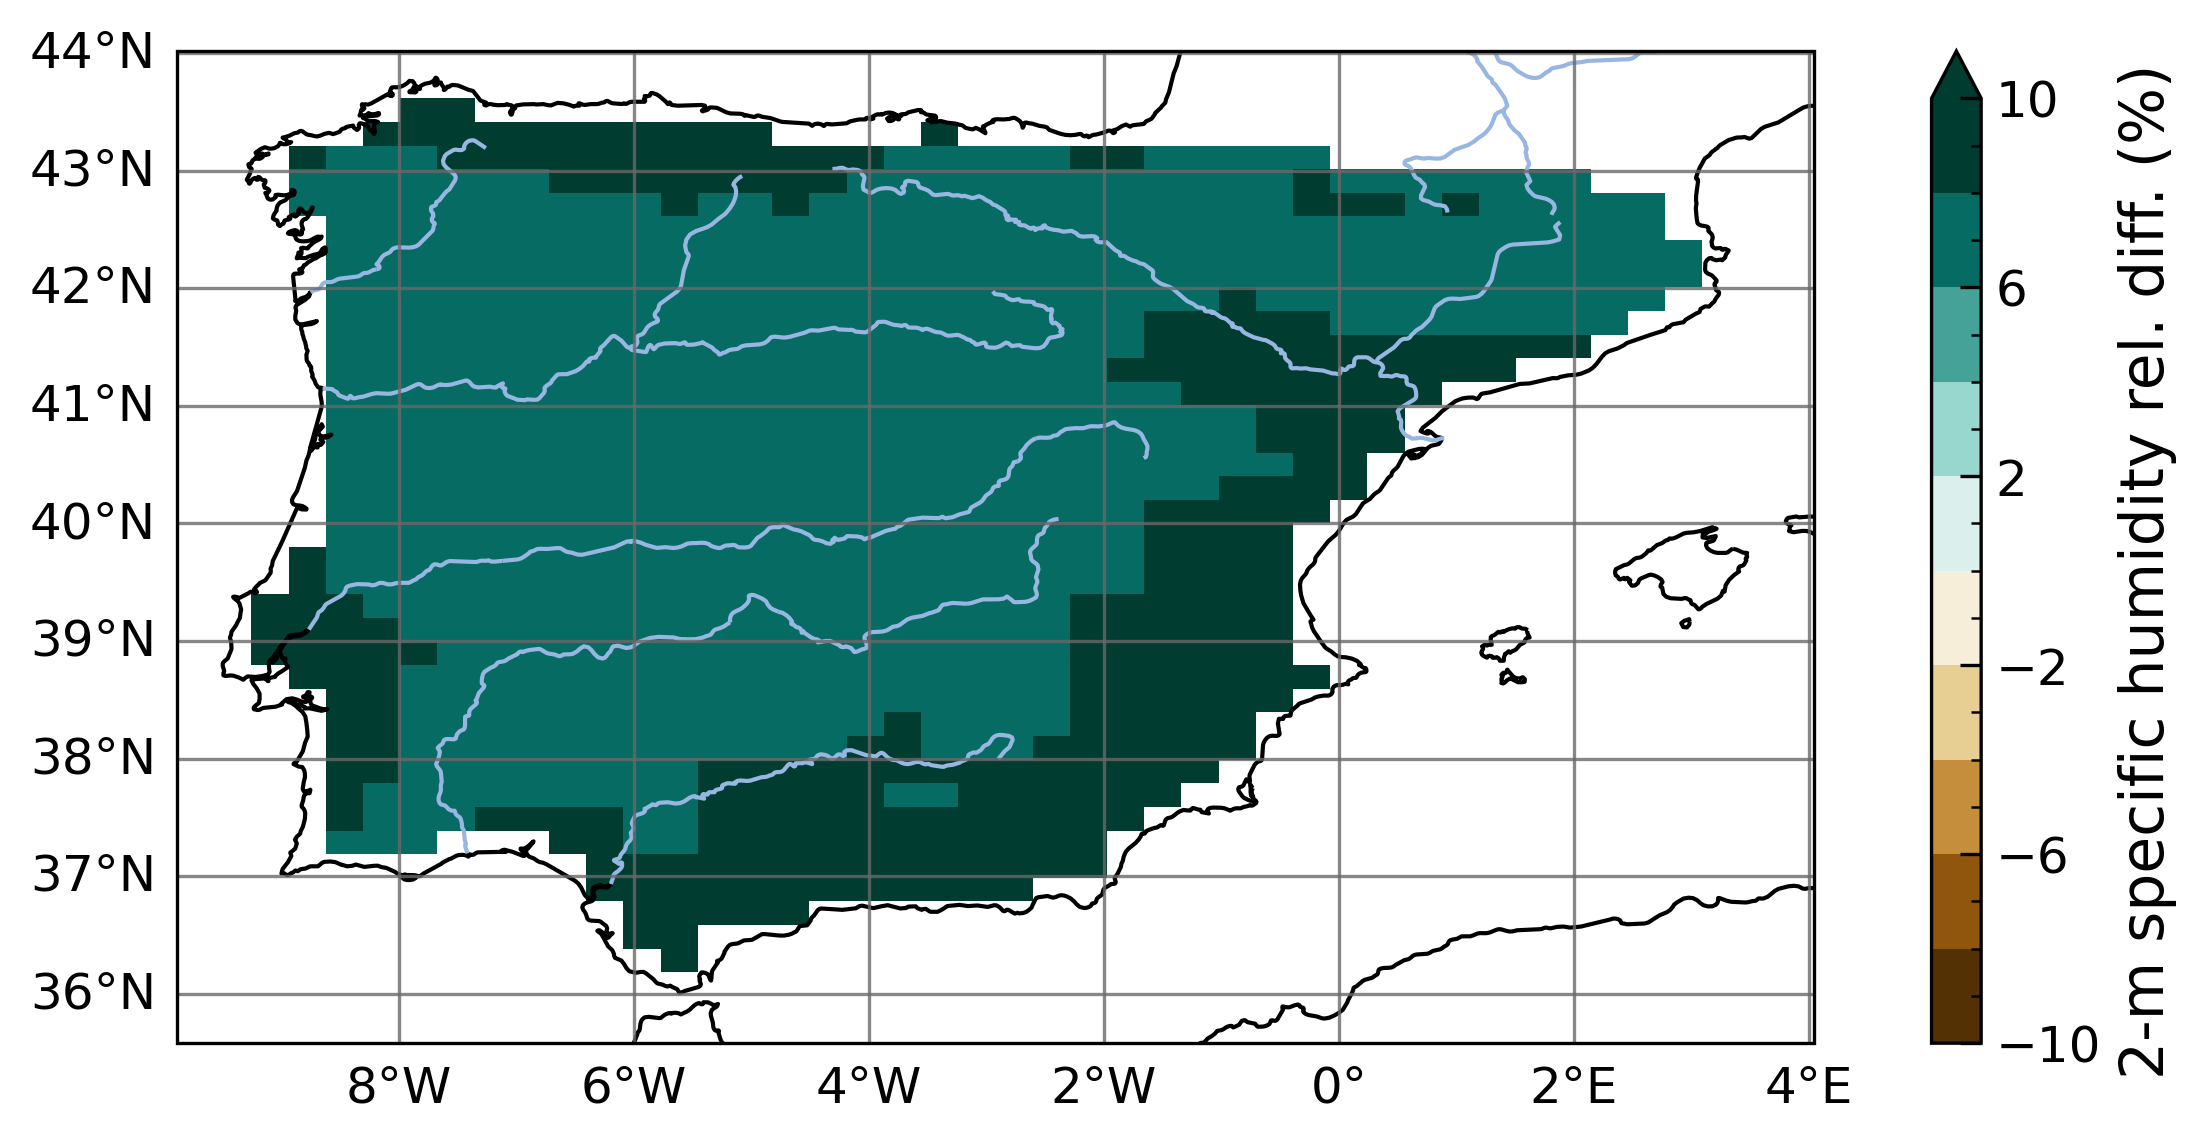
\includegraphics[width=\textwidth]{images/chap4/future/reldiffmap_q2m_presfut.png}
        \end{subfigure} &
        %rh2m
        \begin{subfigure}[b]{0.5\textwidth}
            \caption{}
            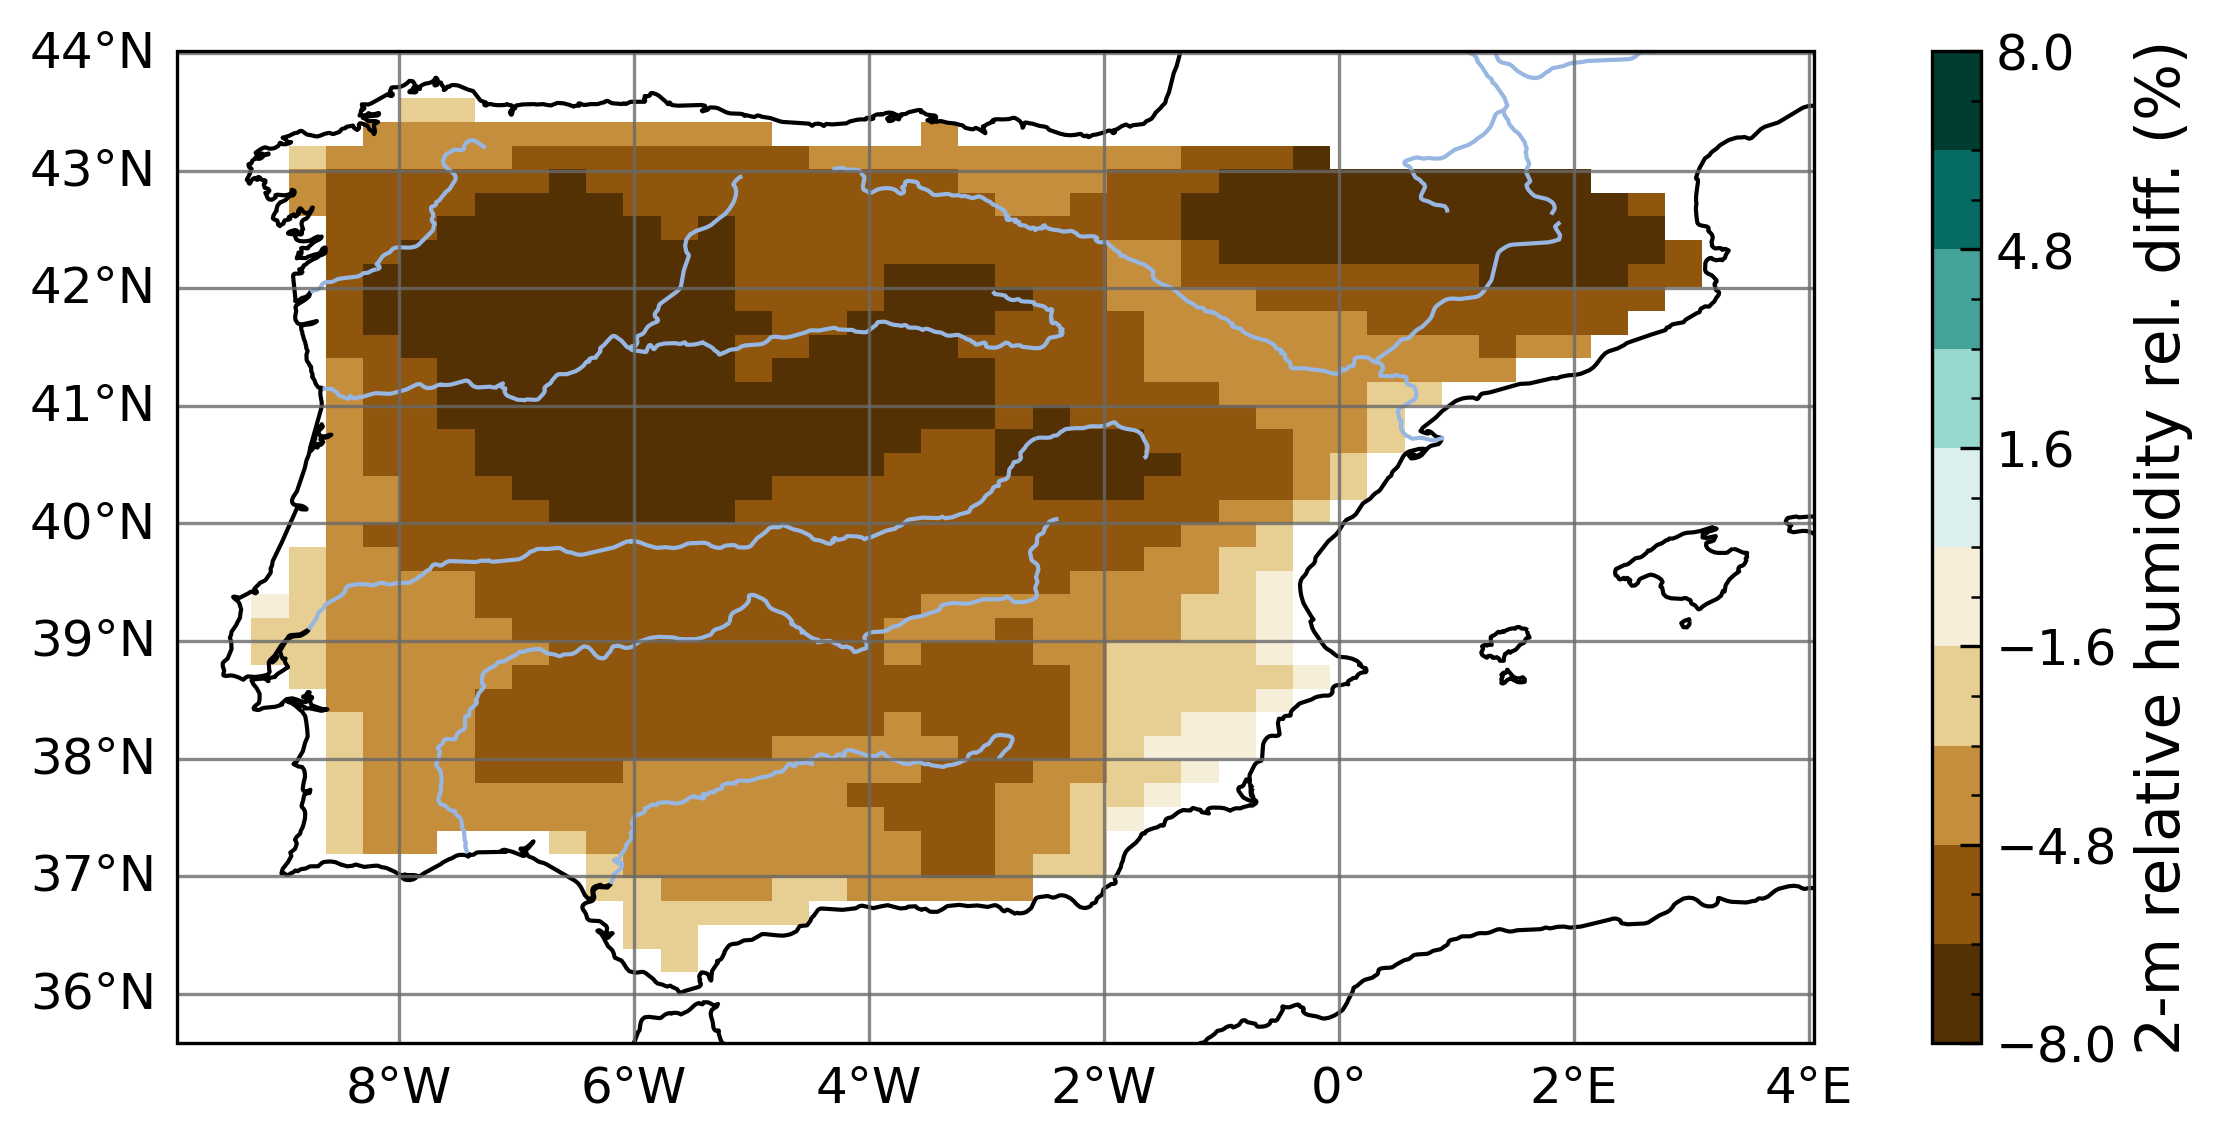
\includegraphics[width=\textwidth]{images/chap4/future/reldiffmap_rh2m_presfut.png}
        \end{subfigure} \\

        %pblh
        \begin{subfigure}[b]{0.5\textwidth}
            \caption{}
            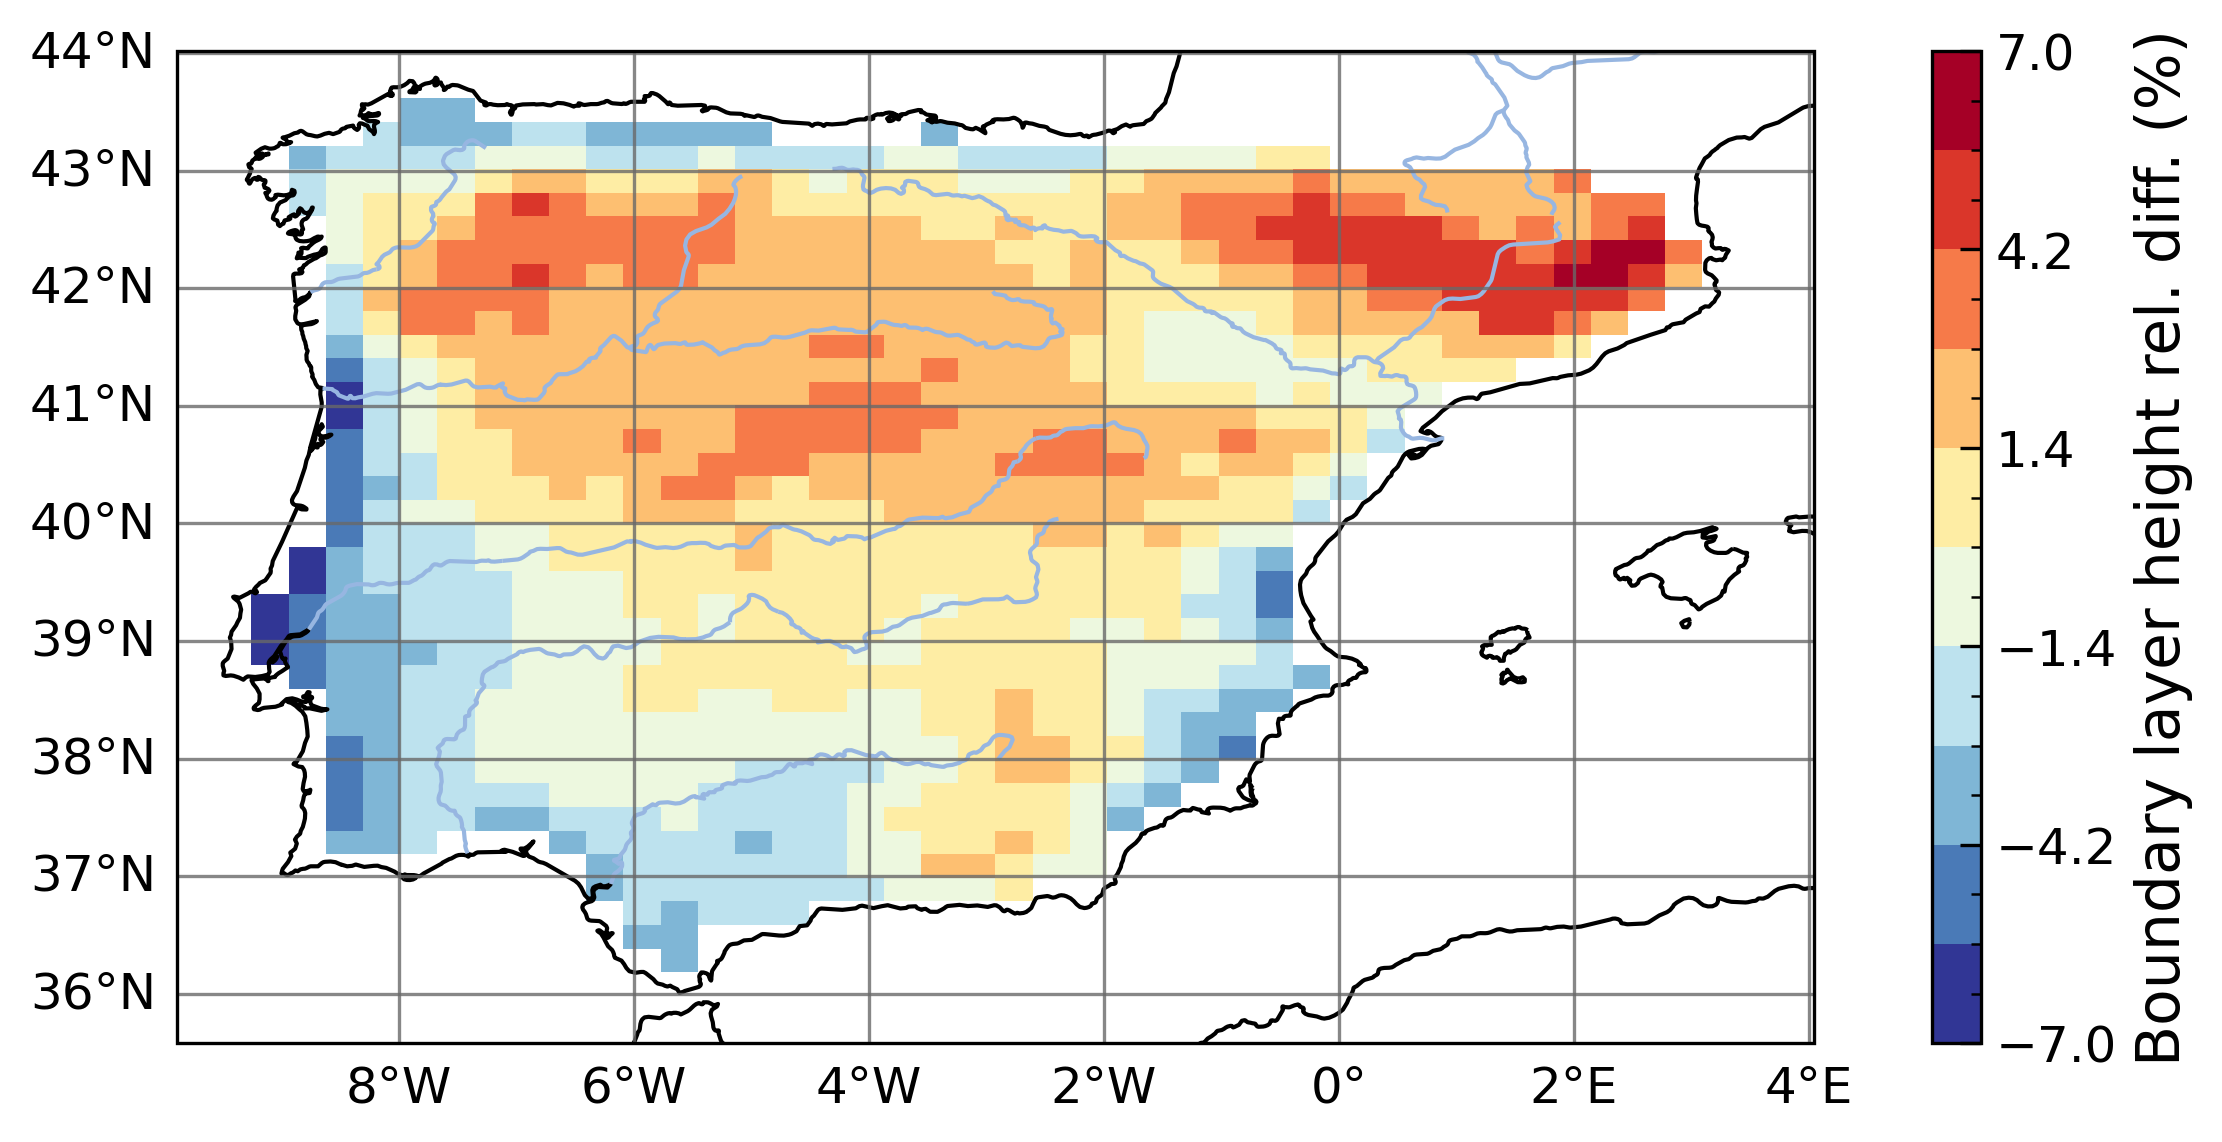
\includegraphics[width=\textwidth]{images/chap4/future/reldiffmap_s_pblh_presfut.png}
        \end{subfigure} &
        %lcl
        \begin{subfigure}[b]{0.5\textwidth}
            \caption{}
            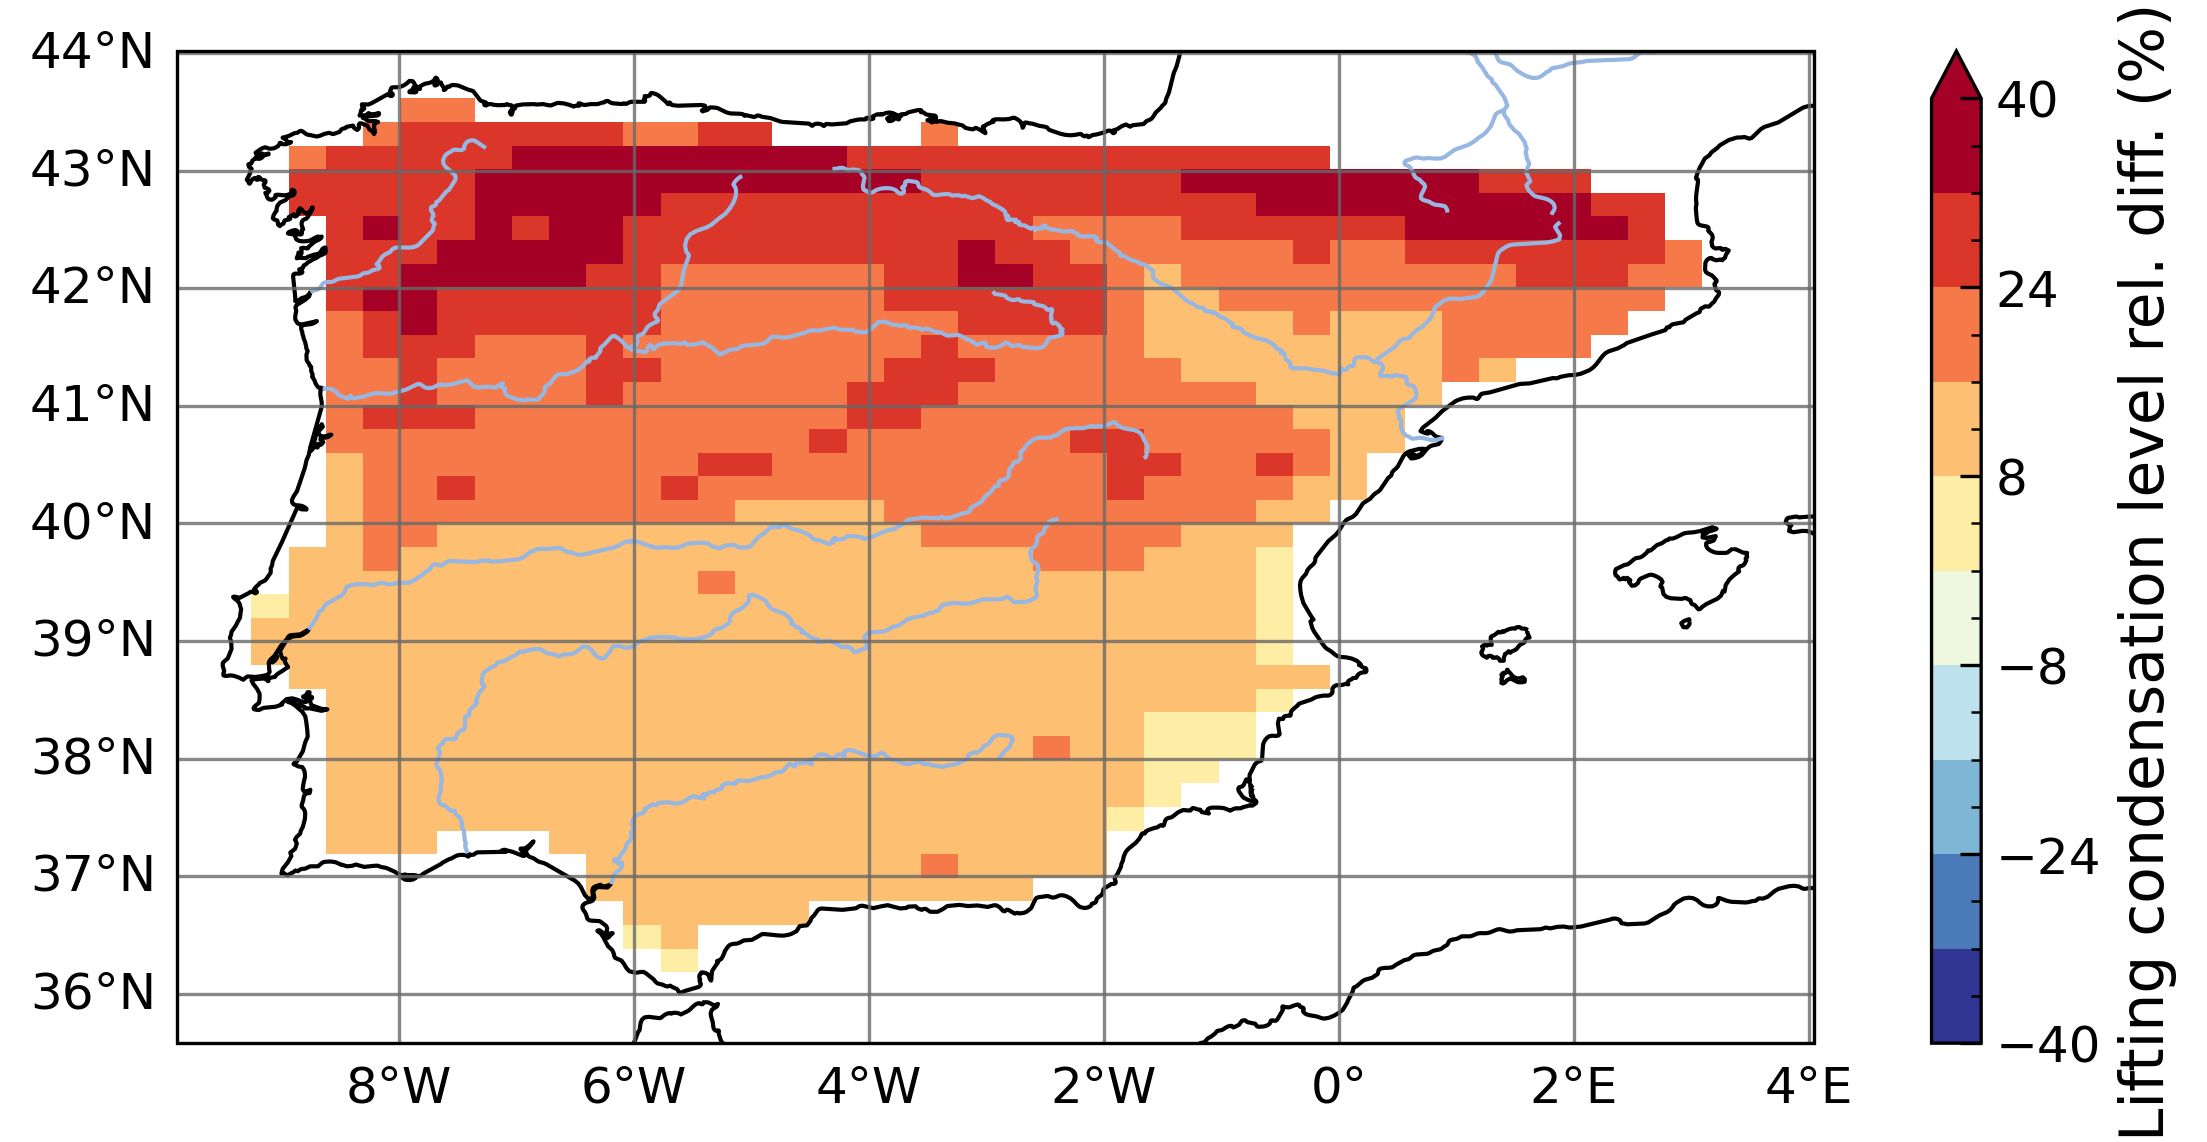
\includegraphics[width=\textwidth]{images/chap4/future/reldiffmap_s_lcl_presfut.png}
        \end{subfigure} \\
    \end{tabular}
    \caption{Relative difference, \futnoirr - \presnoirr}
    \label{fig:reldiffmaps_present_future}
\end{figure}

%figure : diff maps JJA (future, irr - no_irr)
% \begin{figure}[htbp]
%     \centering
%     \begin{tabular}{cc}
%         %precip
%         \begin{subfigure}[b]{0.5\textwidth}
%             \caption{}
%             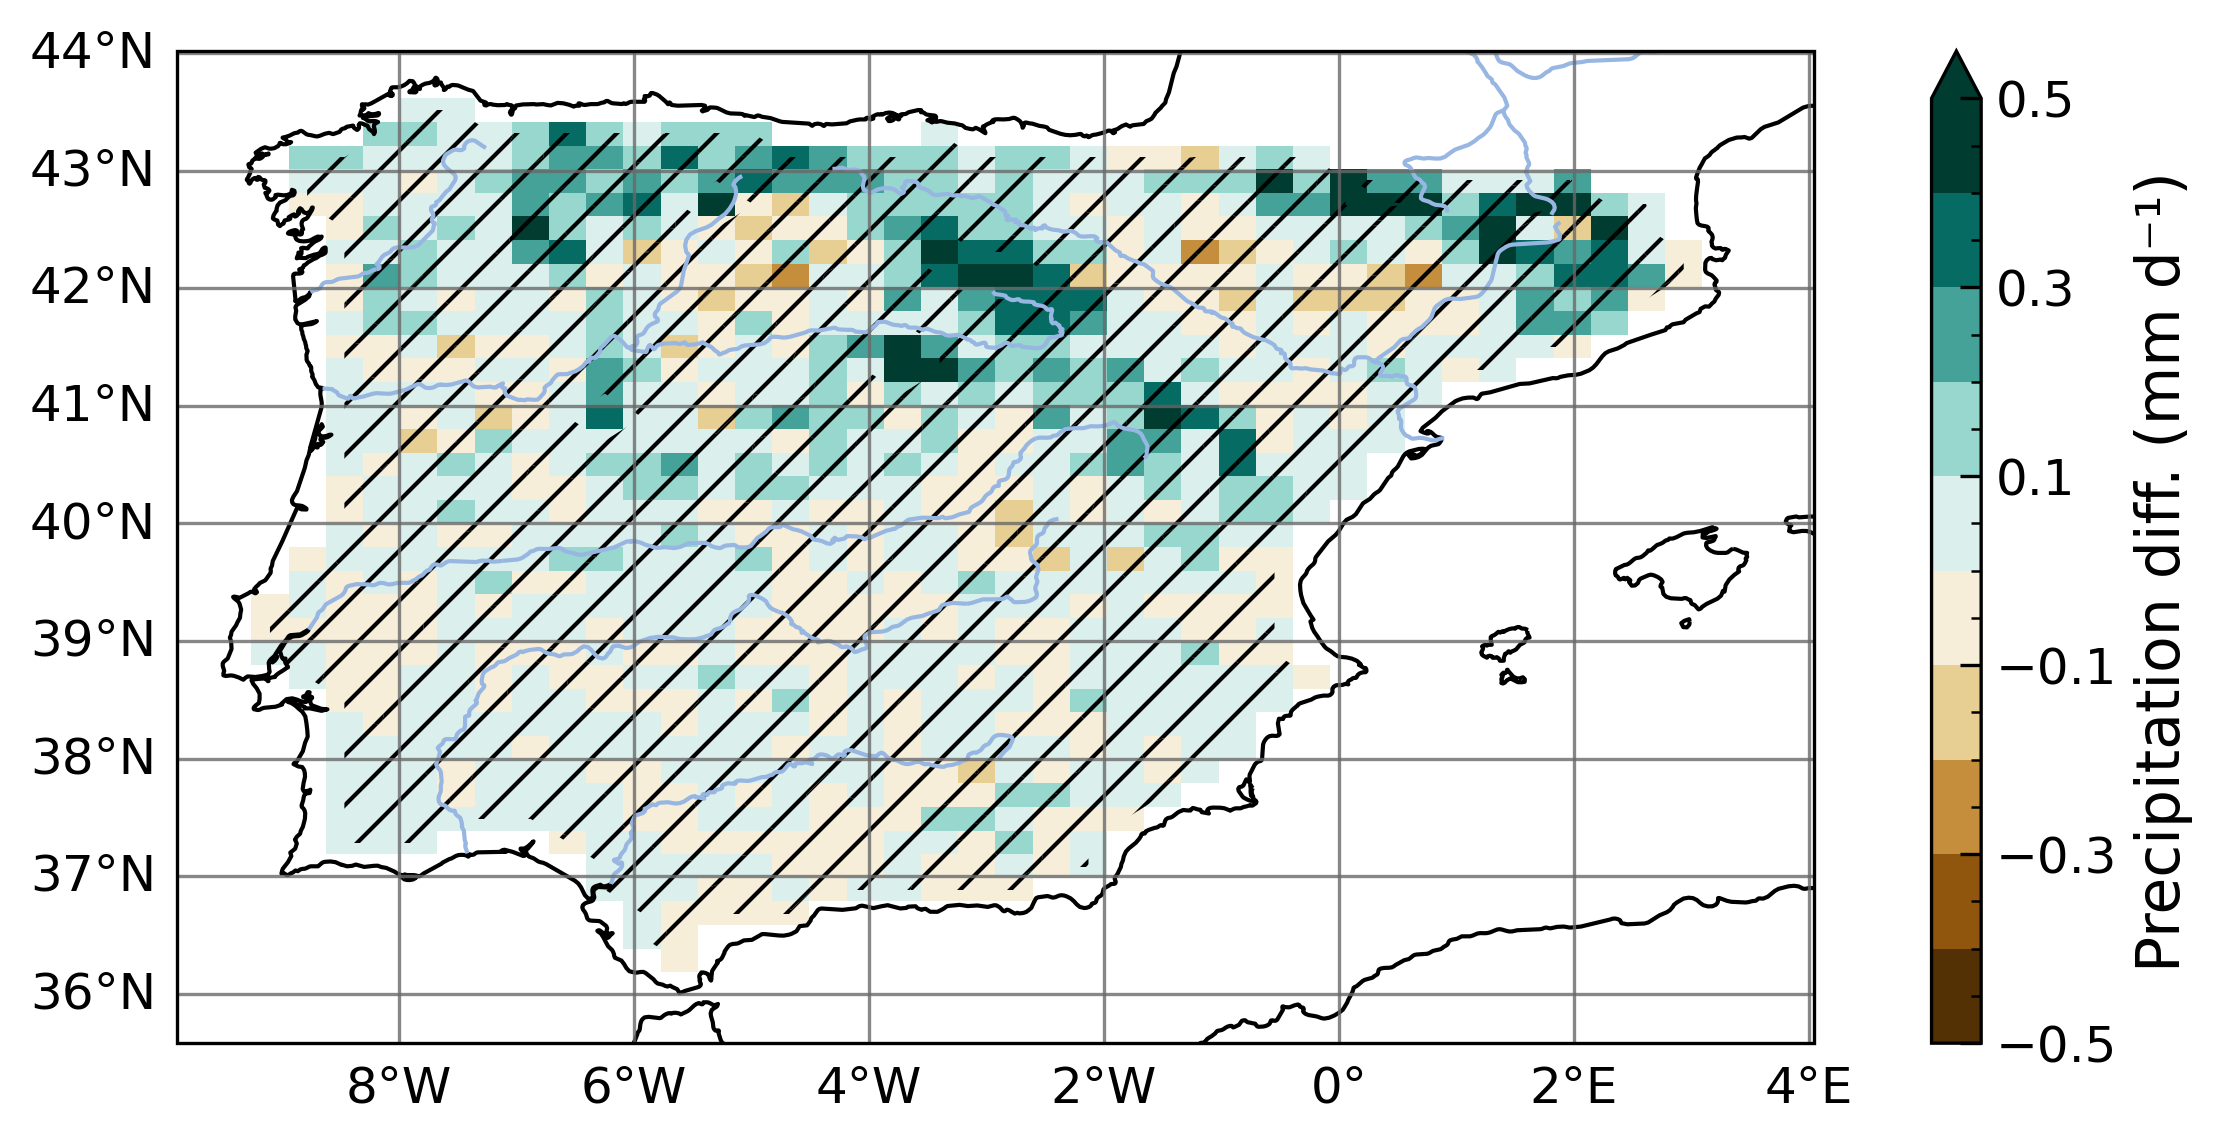
\includegraphics[width=\textwidth]{images/chap4/future/diffmap_JJA_precip_futirr.png}
%         \end{subfigure} &
%         %evap
%         \begin{subfigure}[b]{0.5\textwidth}
%             \caption{}
%             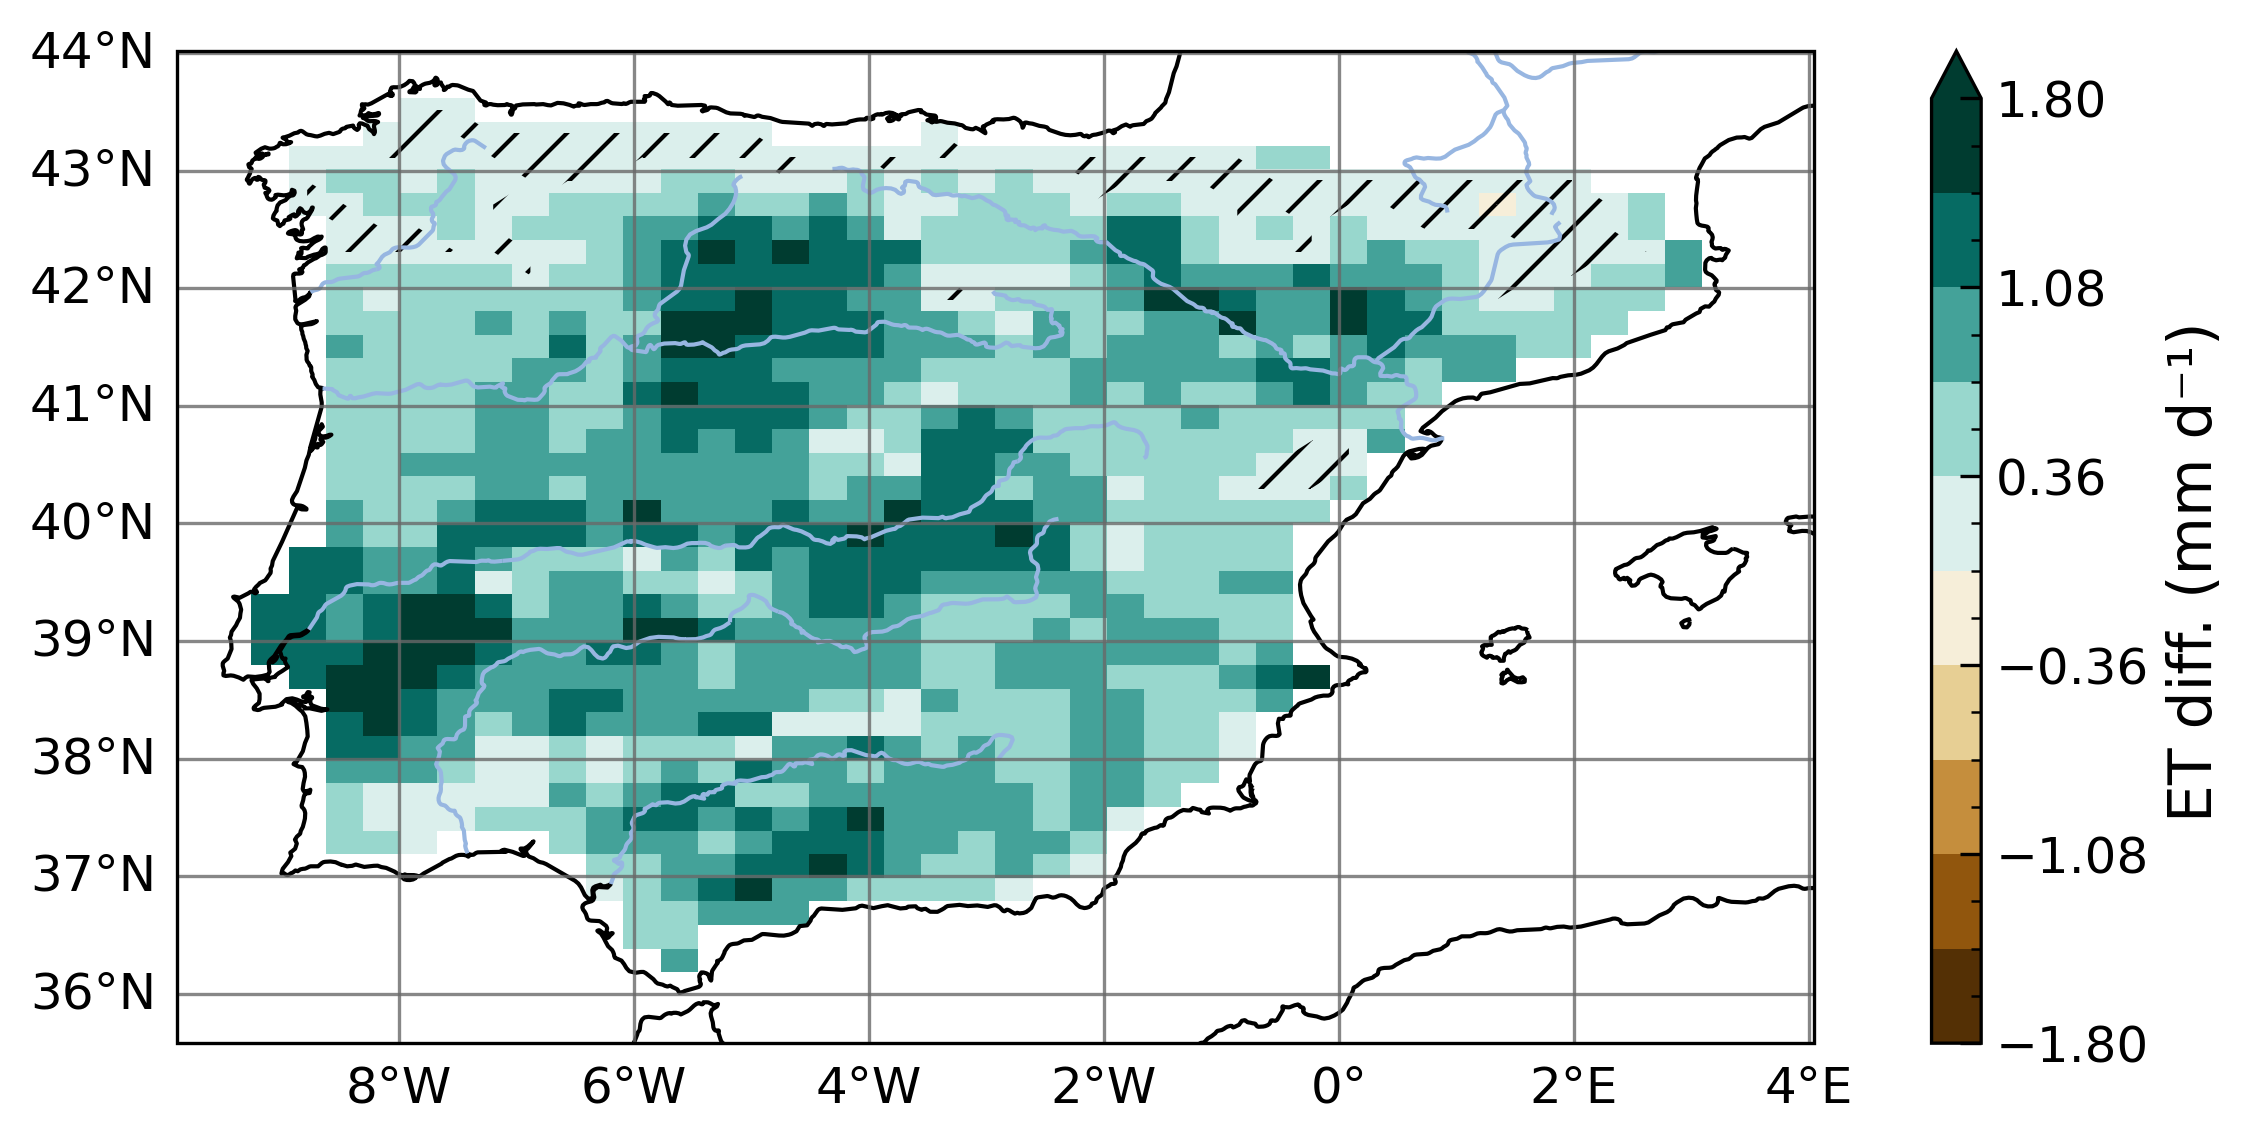
\includegraphics[width=\textwidth]{images/chap4/future/diffmap_JJA_evap_futirr.png}
%         \end{subfigure} \\

%         %t2m
%         \begin{subfigure}[b]{0.5\textwidth}
%             \caption{}
%             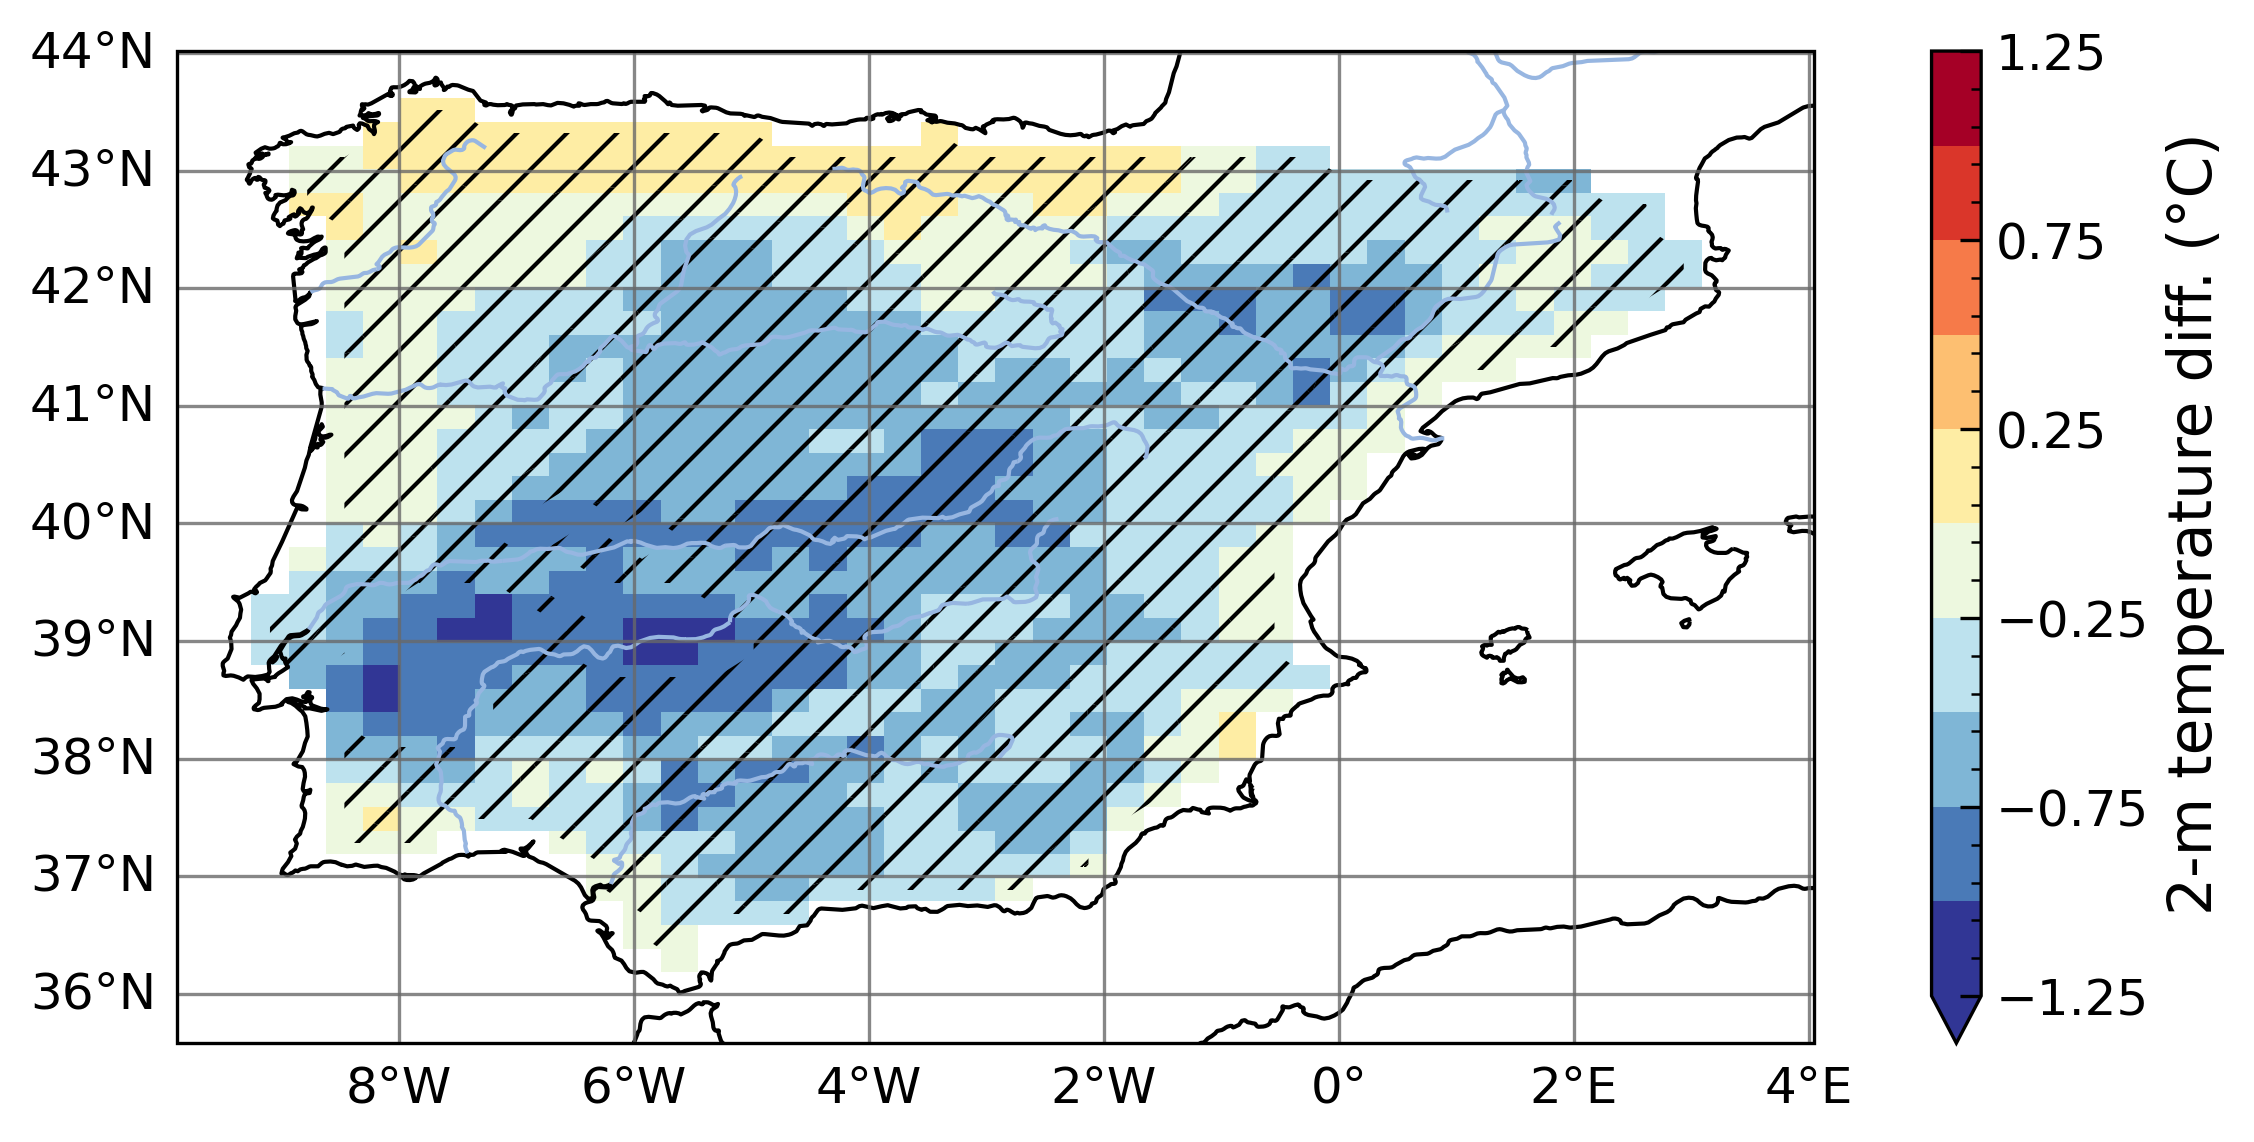
\includegraphics[width=\textwidth]{images/chap4/future/diffmap_JJA_t2m_futirr.png}
%         \end{subfigure} &
%         %fluxsens
%         \begin{subfigure}[b]{0.5\textwidth}
%             \caption{}
%             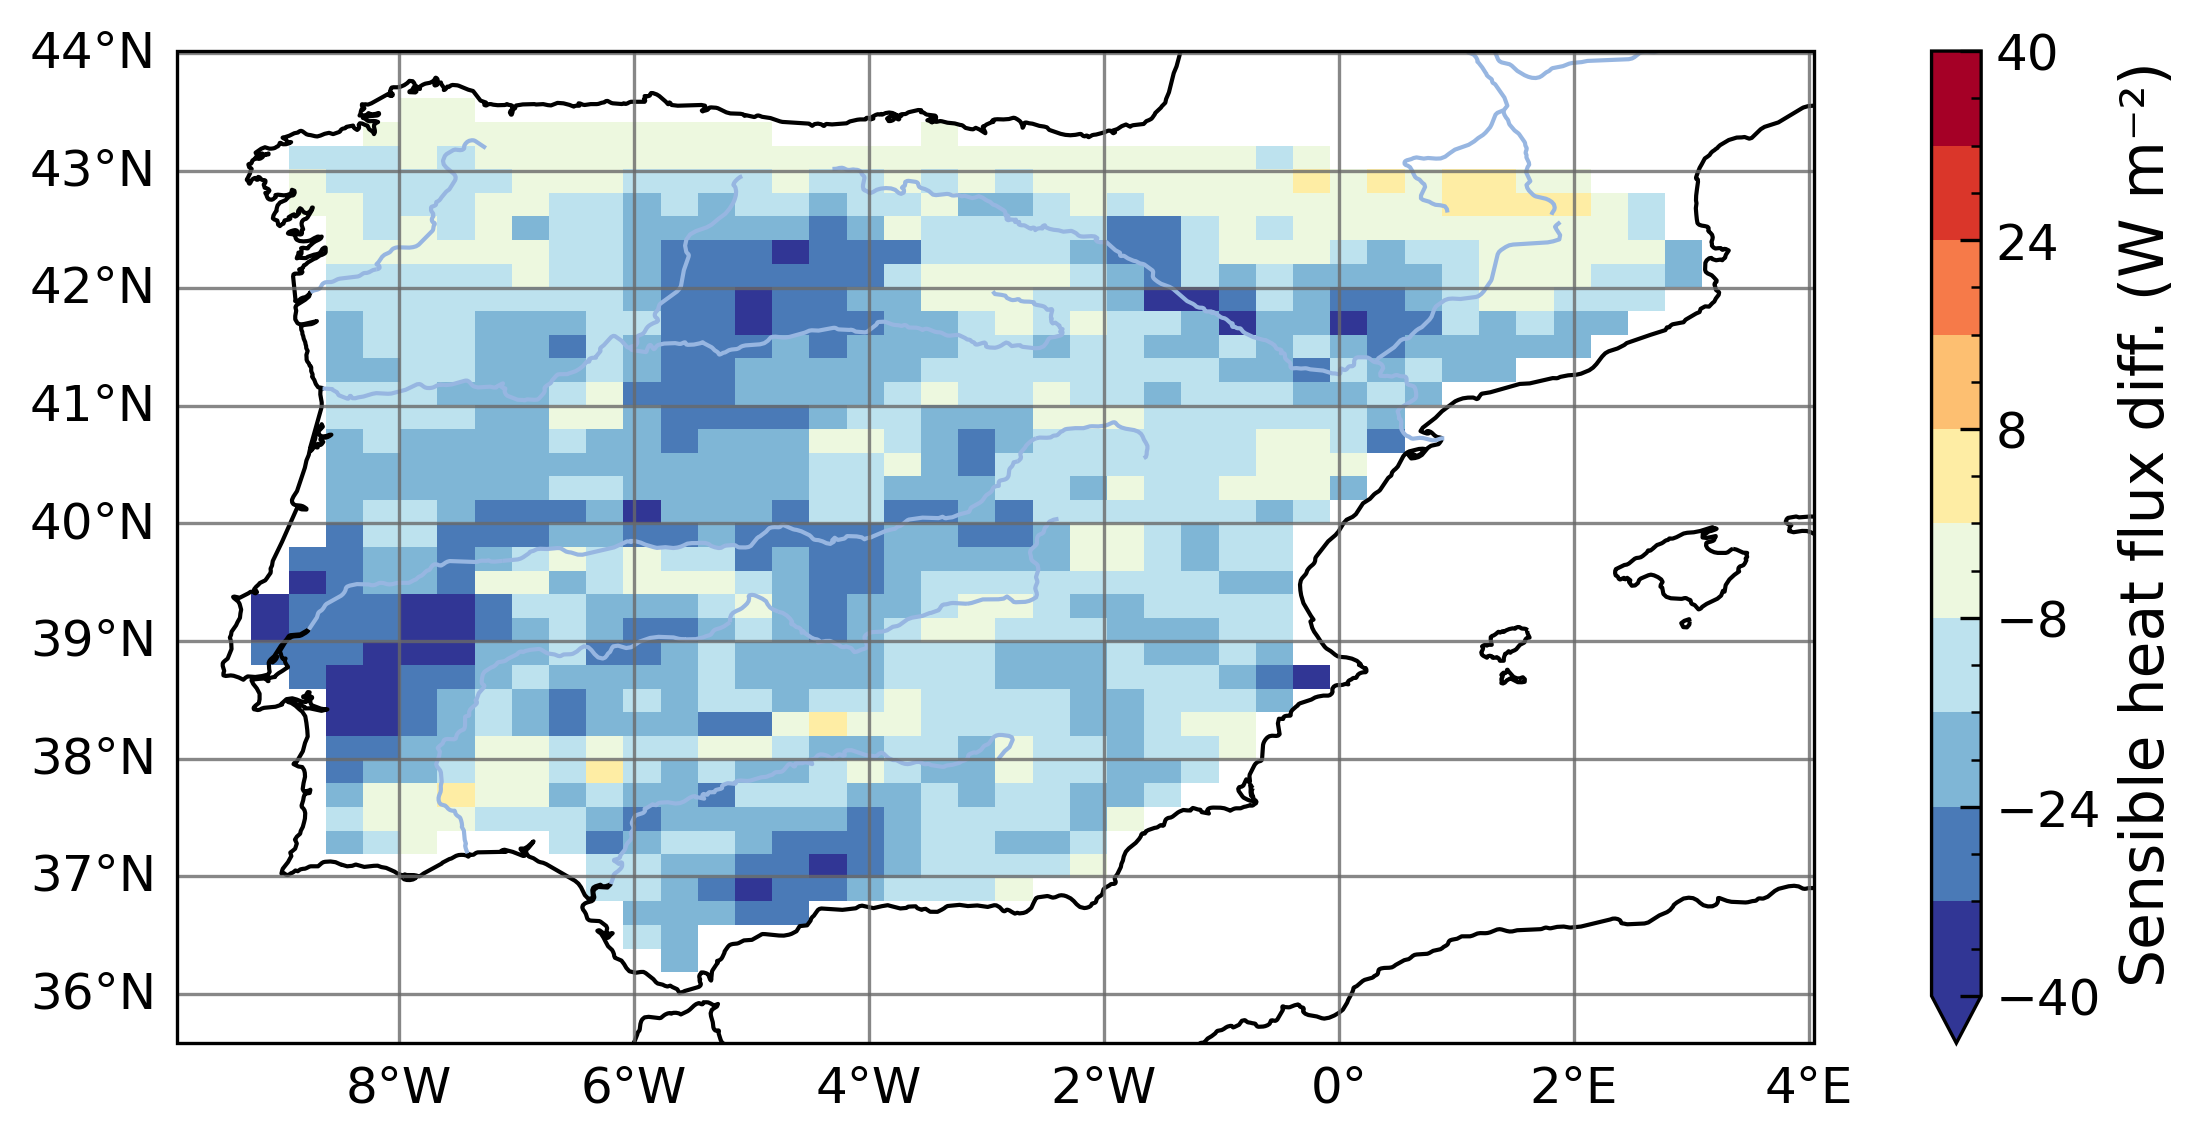
\includegraphics[width=\textwidth]{images/chap4/future/diffmap_JJA_fluxsens_futirr.png}
%         \end{subfigure} \\

%         %q2m
%         \begin{subfigure}[b]{0.5\textwidth}
%             \caption{}
%             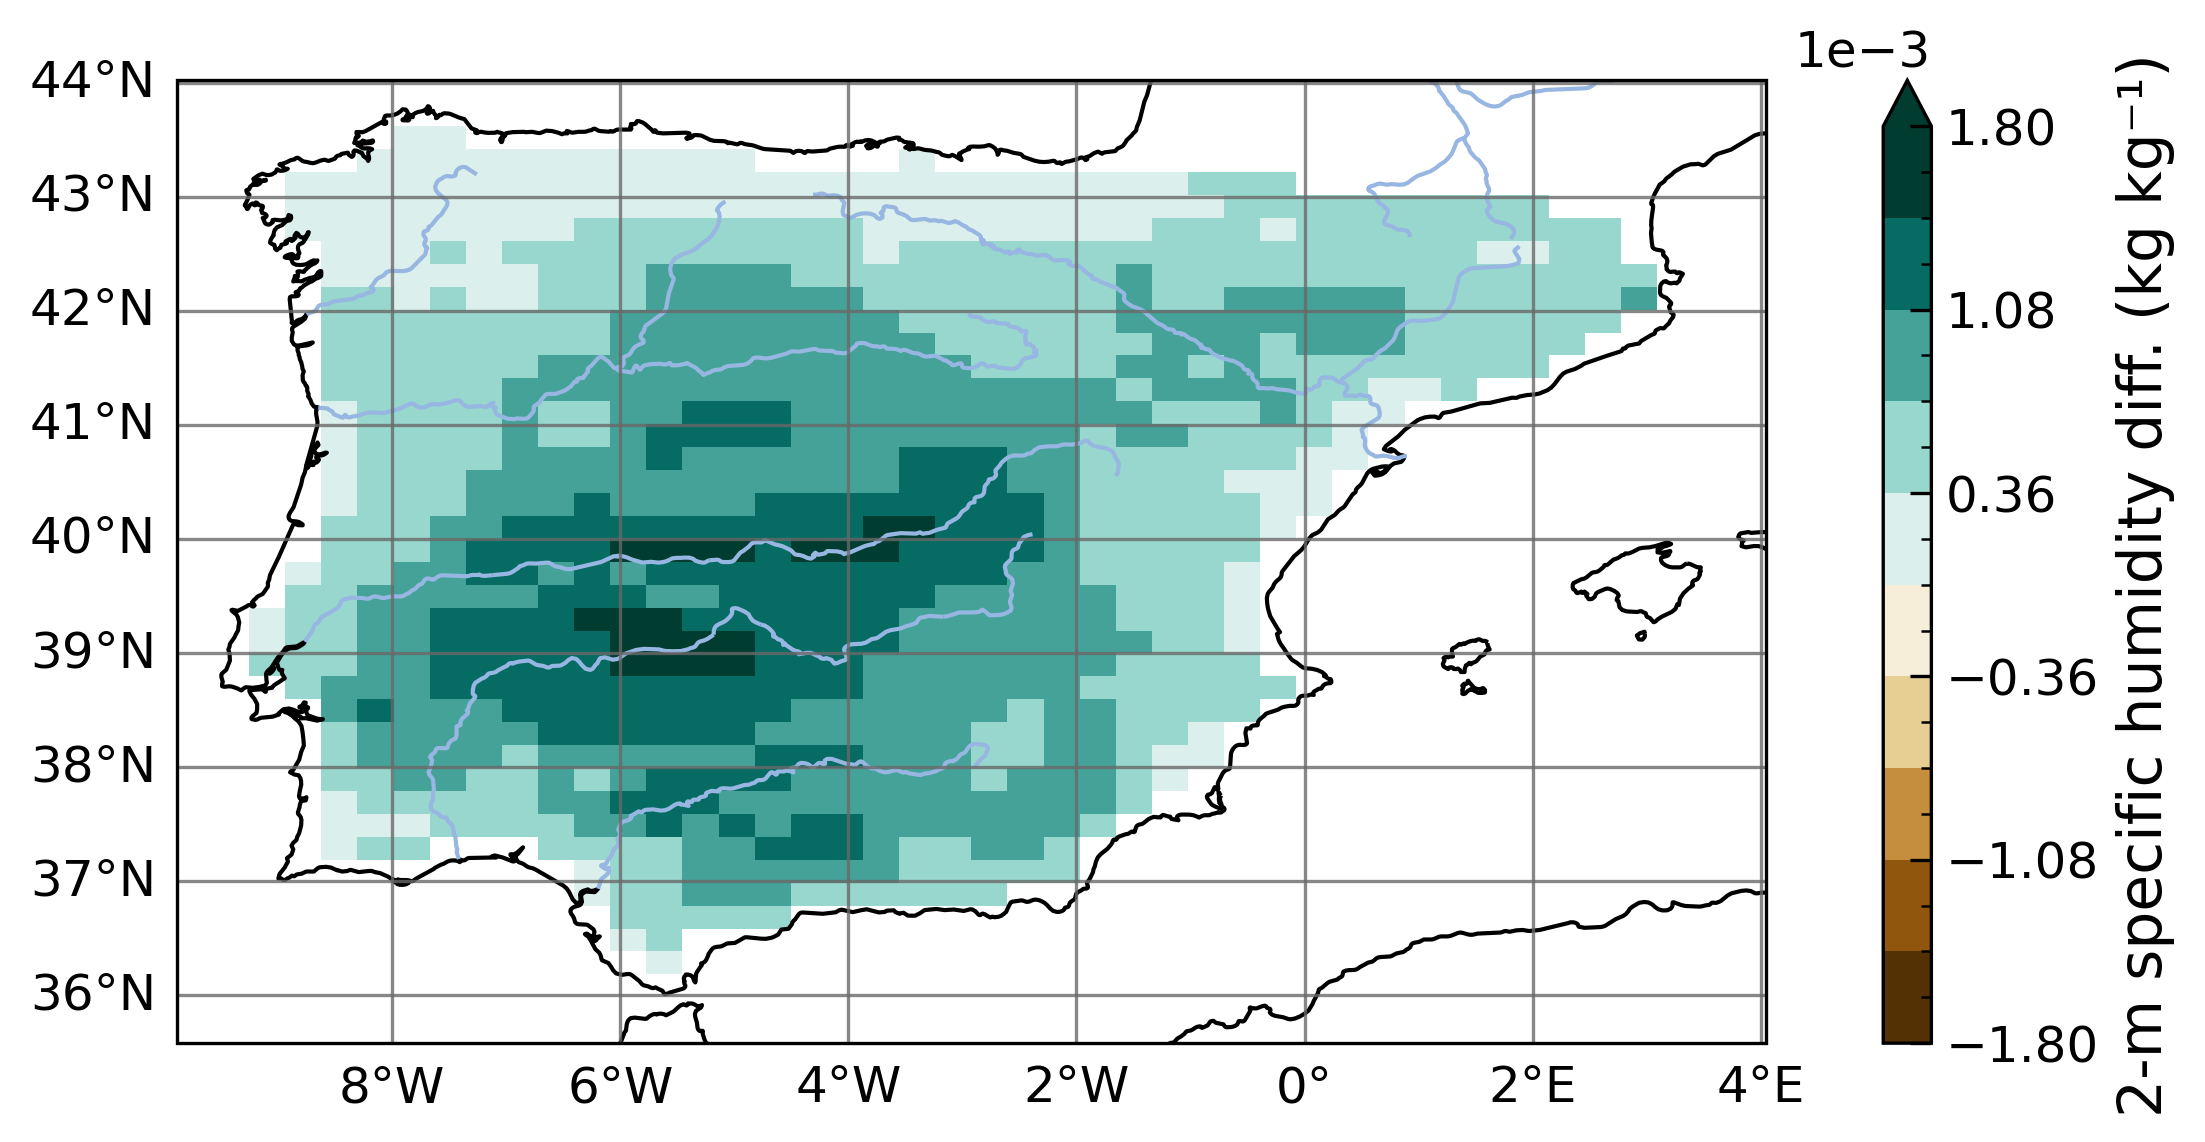
\includegraphics[width=\textwidth]{images/chap4/future/diffmap_JJA_q2m_futirr.png}
%         \end{subfigure} &
%         %rh2m
%         \begin{subfigure}[b]{0.5\textwidth}
%             \caption{}
%             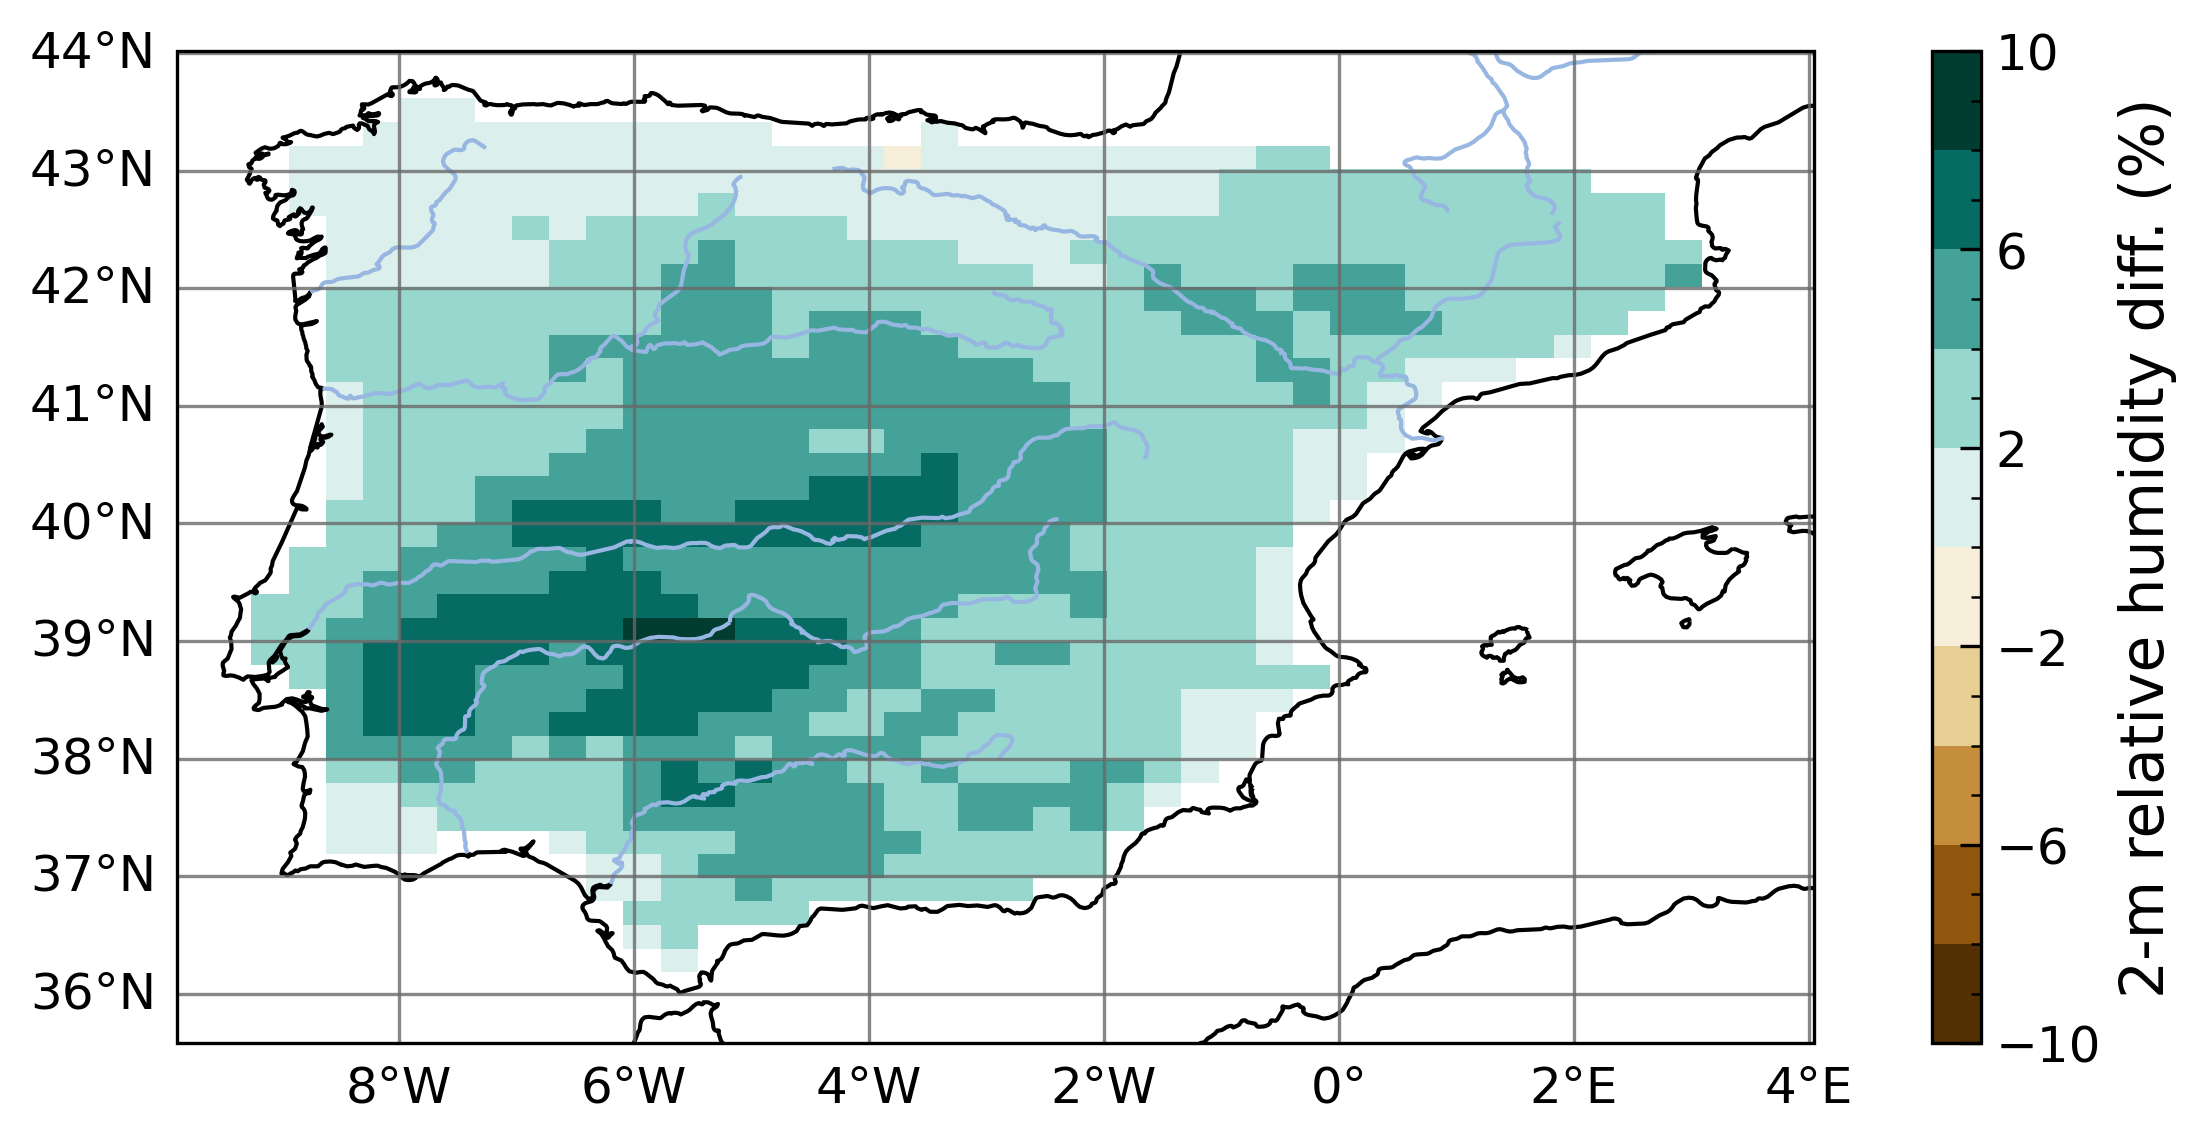
\includegraphics[width=\textwidth]{images/chap4/future/diffmap_JJA_rh2m_futirr.png}
%         \end{subfigure} \\

%         %pblh
%         \begin{subfigure}[b]{0.5\textwidth}
%             \caption{}
%             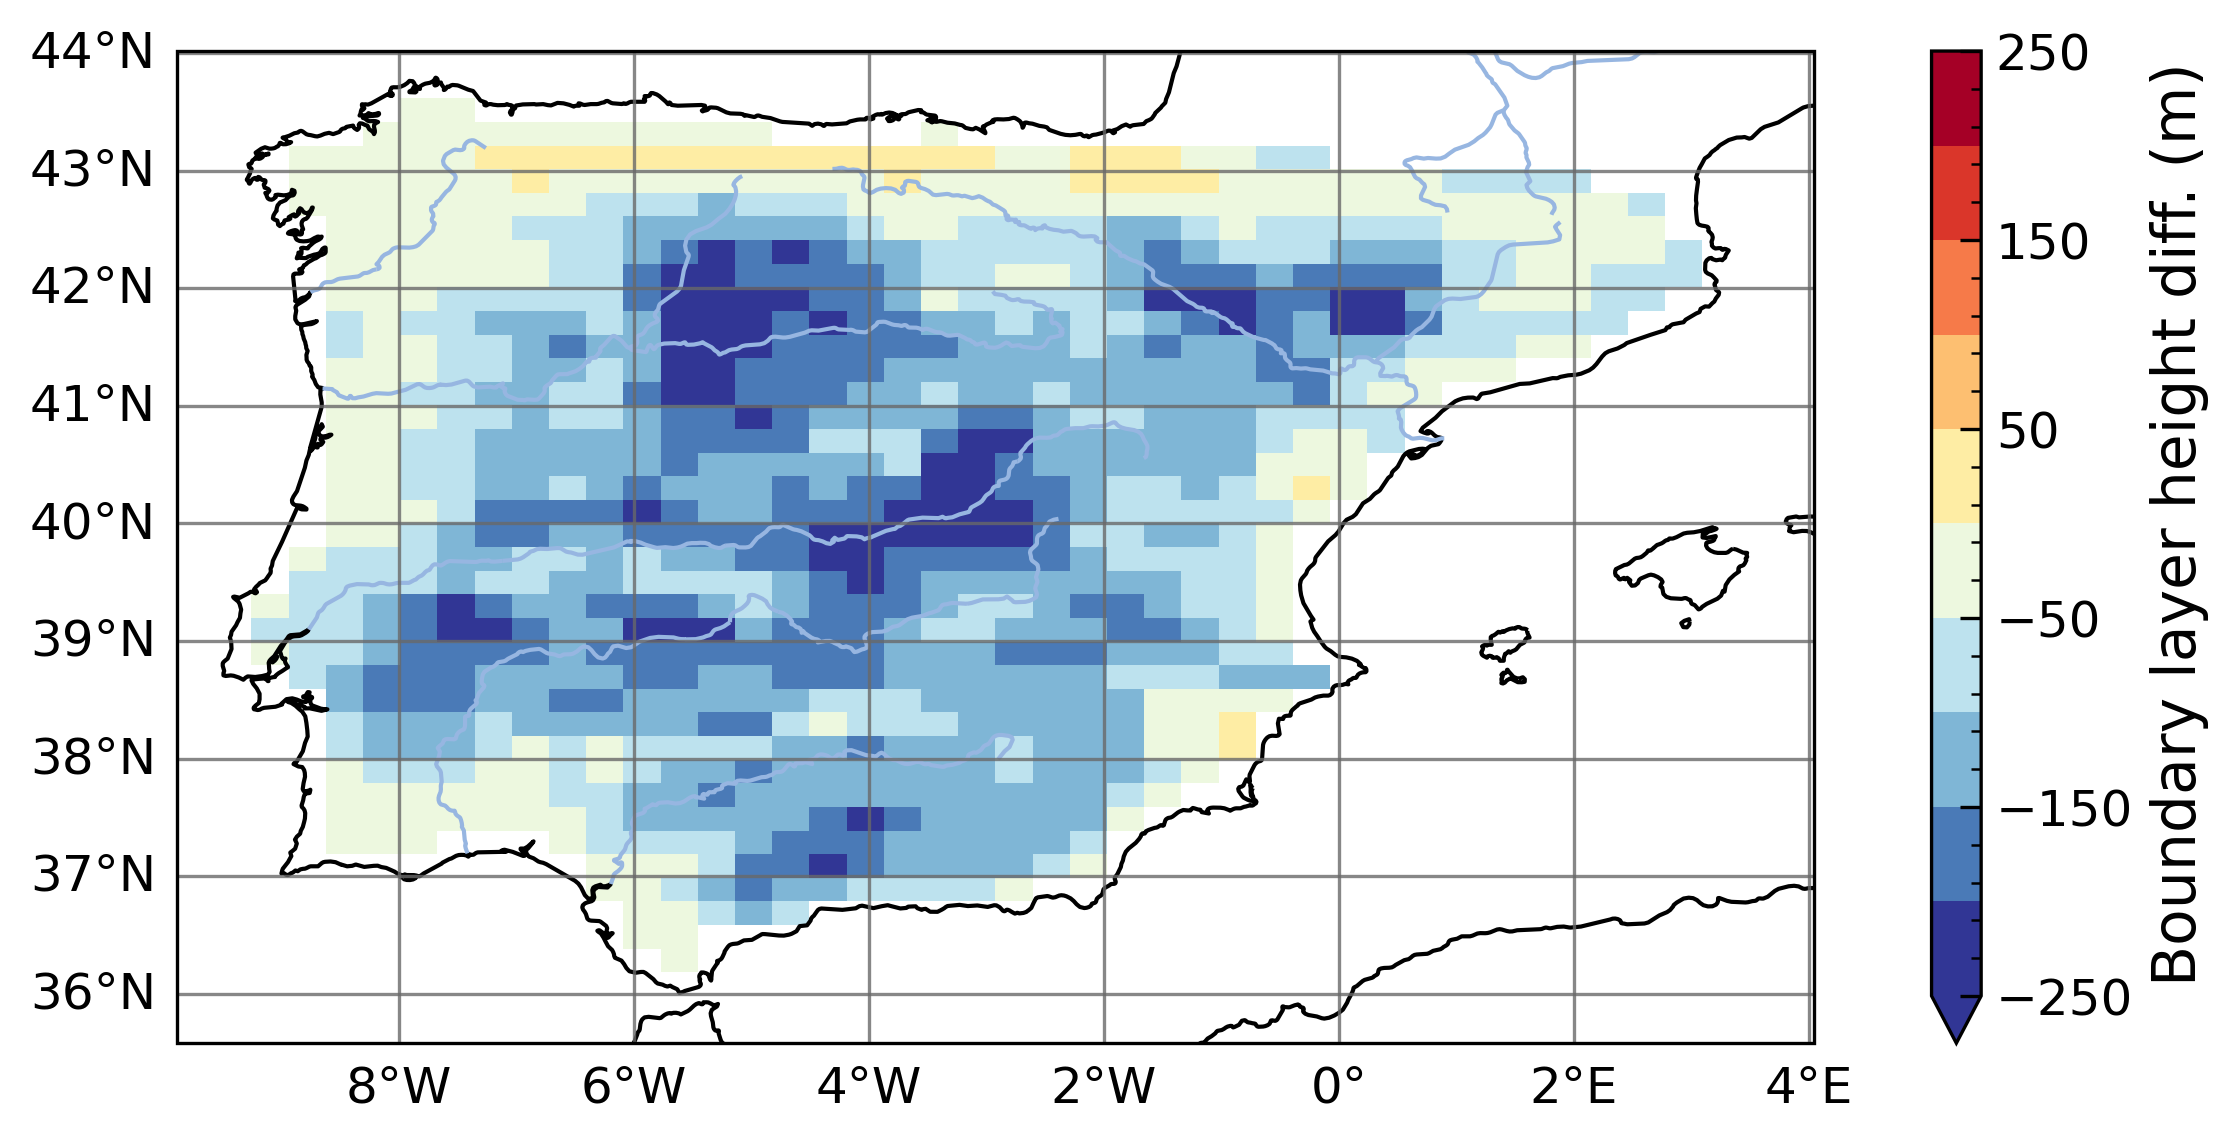
\includegraphics[width=\textwidth]{images/chap4/future/diffmap_JJA_s_pblh_futirr.png}
%         \end{subfigure} &
%         %lcl
%         \begin{subfigure}[b]{0.5\textwidth}
%             \caption{}
%             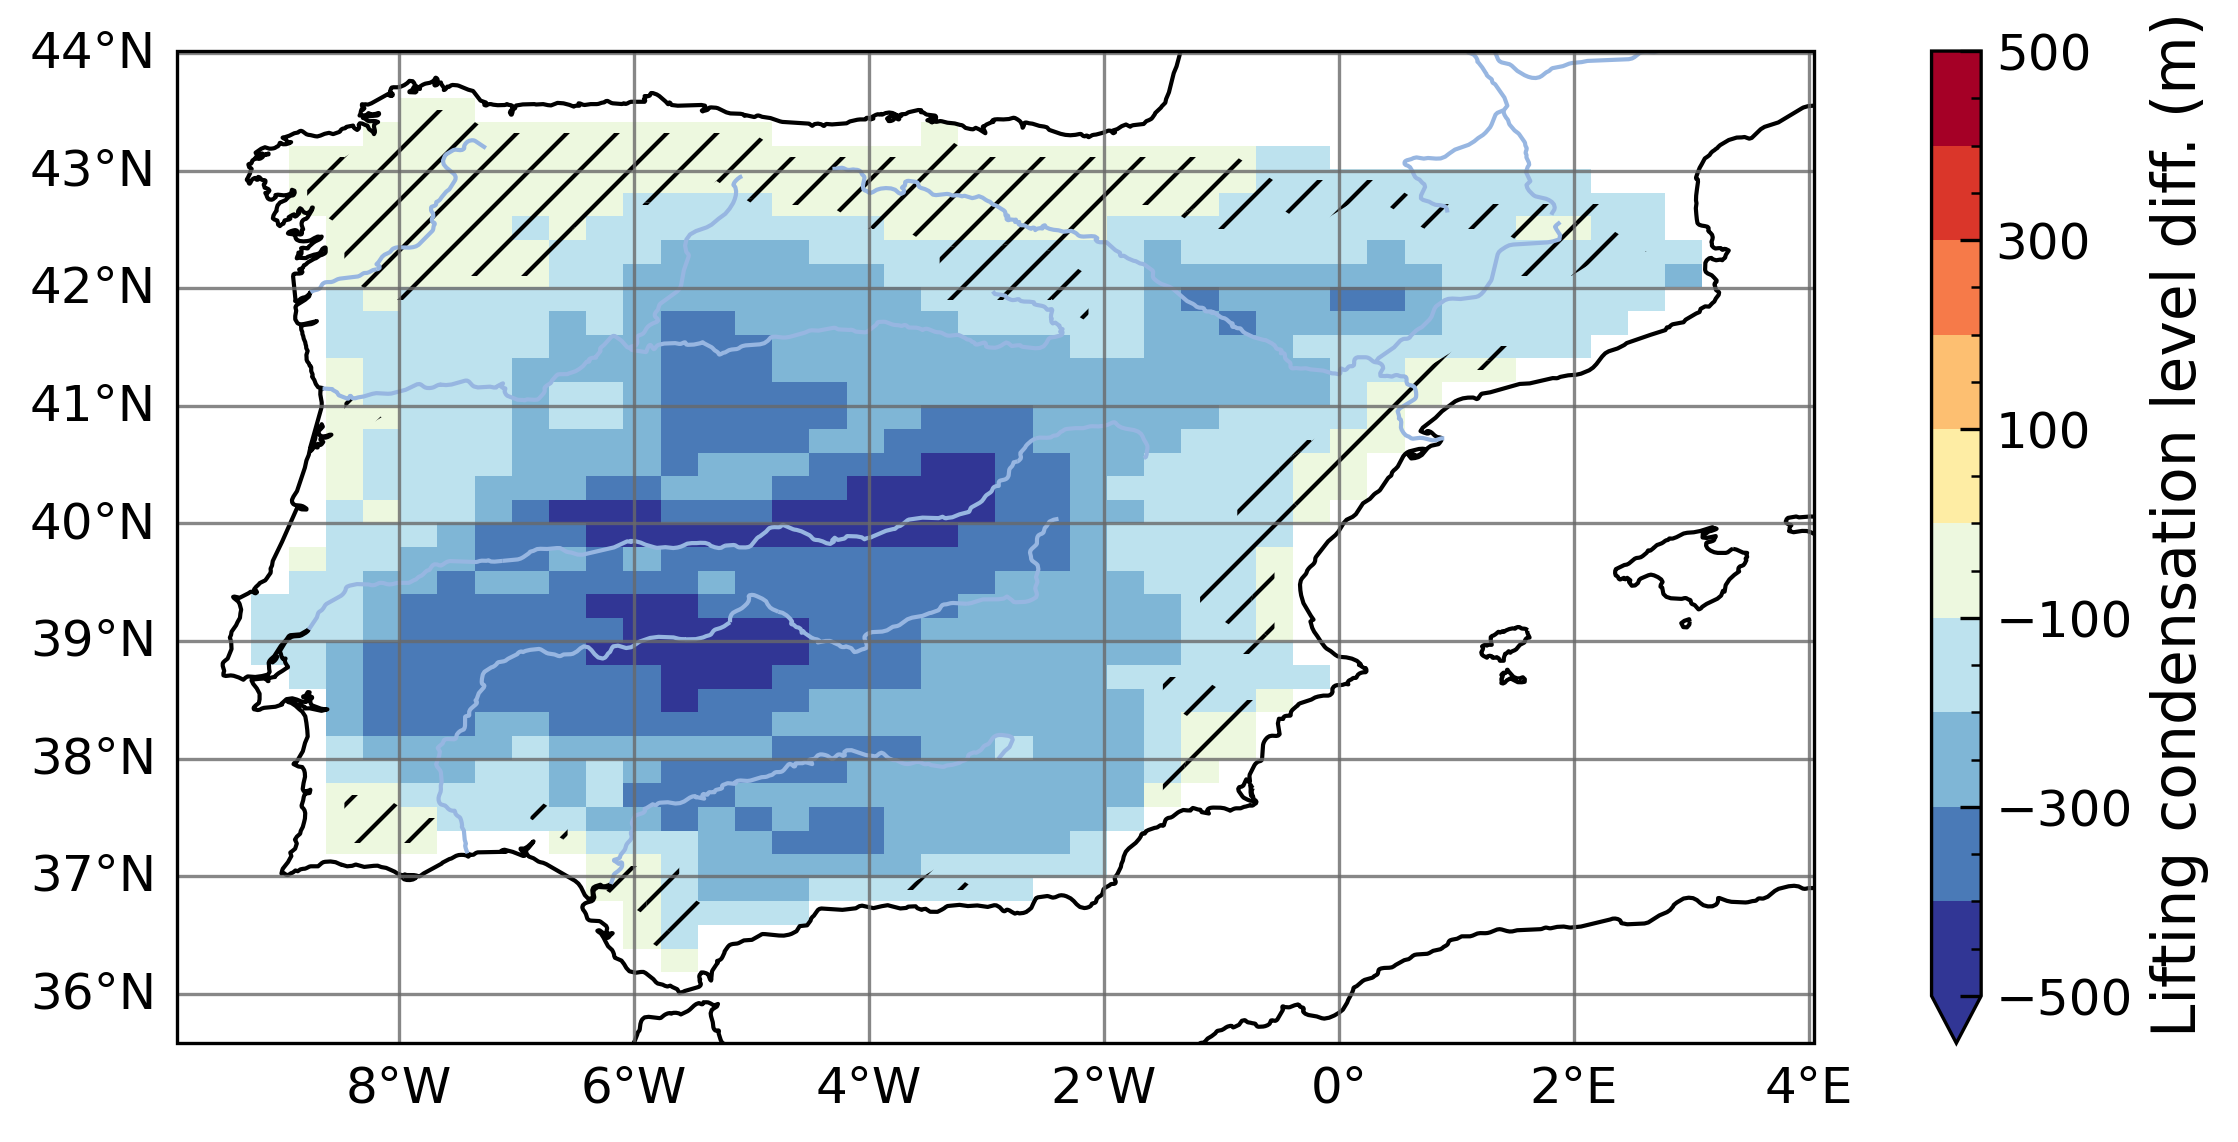
\includegraphics[width=\textwidth]{images/chap4/future/diffmap_JJA_s_lcl_futirr.png}
%         \end{subfigure} \\
%     \end{tabular}
%     \caption{JJA difference (\futnoirr - \futirr)}
%     \label{fig:diffmaps_JJA_future_irr}
% \end{figure}


%figure : rel diff maps (future, irr - no_irr)
\begin{figure}[htbp]
    \centering
    \begin{tabular}{cc}
        %precip
        \begin{subfigure}[b]{0.5\textwidth}
            \caption{}
            \includegraphics[width=\textwidth]{images/chap4/future/reldiffmap_precip_futirr.png}
        \end{subfigure} &
        %evap
        \begin{subfigure}[b]{0.5\textwidth}
            \caption{}
            \includegraphics[width=\textwidth]{images/chap4/future/reldiffmap_evap_futirr.png}
        \end{subfigure} \\

        %t2m
        \begin{subfigure}[b]{0.5\textwidth}
            \caption{}
            \includegraphics[width=\textwidth]{images/chap4/future/reldiffmap_psol_futirr.png}
        \end{subfigure} &
        %fluxsens
        \begin{subfigure}[b]{0.5\textwidth}
            \caption{}
            \includegraphics[width=\textwidth]{images/chap4/future/reldiffmap_fluxsens_futirr.png}
        \end{subfigure} \\

        %q2m
        \begin{subfigure}[b]{0.5\textwidth}
            \caption{}
            \includegraphics[width=\textwidth]{images/chap4/future/reldiffmap_q2m_futirr.png}
        \end{subfigure} &
        %rh2m
        \begin{subfigure}[b]{0.5\textwidth}
            \caption{}
            \includegraphics[width=\textwidth]{images/chap4/future/reldiffmap_rh2m_futirr.png}
        \end{subfigure} \\

        %pblh
        \begin{subfigure}[b]{0.5\textwidth}
            \caption{}
            \includegraphics[width=\textwidth]{images/chap4/future/reldiffmap_s_pblh_futirr.png}
        \end{subfigure} &
        %lcl
        \begin{subfigure}[b]{0.5\textwidth}
            \caption{}
            \includegraphics[width=\textwidth]{images/chap4/future/reldiffmap_s_lcl_futirr.png}
        \end{subfigure} \\
    \end{tabular}
    \caption{Annual relative difference (\futnoirr - \futirr)}
    \label{fig:reldiffmaps_future_irr}
\end{figure}

%figure : Aridity Index diff and rel diff maps
\begin{figure}[htbp]
    \centering
    \begin{tabular}{cc}
        %present vs future (noirr)
        \begin{subfigure}[b]{0.5\textwidth}
            \caption{Absolute change in aridity index under climate change}
            \includegraphics[width=\textwidth]{images/chap4/future/diffmap_aridity_index_presfut.png}
        \end{subfigure} &
        \begin{subfigure}[b]{0.5\textwidth}
            \caption{Relative change in aridity index under climate change}
            \includegraphics[width=\textwidth]{images/chap4/future/reldiffmap_aridity_index_presfut.png}
        \end{subfigure} \\

        %irr vs noirr (future)
        \begin{subfigure}[b]{0.5\textwidth}
            \caption{Absolute change in future aridity index in the presence of irrigation}
            \includegraphics[width=\textwidth]{images/chap4/future/diffmap_aridity_index_futirr.png}
        \end{subfigure} &
        \begin{subfigure}[b]{0.5\textwidth}
            \caption{Relative change in future aridity index in the presence of irrigation}
            \includegraphics[width=\textwidth]{images/chap4/future/reldiffmap_aridity_index_futirr.png}
        \end{subfigure} \\
    \end{tabular}
    \caption{Aridity index changes under climate change and in the presence of irrigation.}
    \label{fig:diffmaps_aridity}
\end{figure}

\clearpage

\section*{Appendix to chapter \ref{chap:liaise}}

\begin{figure}[hbtp]
    \centering
    \begin{tabular}{cc}
        \begin{subfigure}[t]{0.5\textwidth}
            \caption{}
            \includegraphics[width=\textwidth]{images/chap6/SOP_TS_DC/time_series_cendrosa_SWdnSFC.png}
        \end{subfigure} &
        \begin{subfigure}[t]{0.5\textwidth}
            \caption{}
            \includegraphics[width=\textwidth]{images/chap6/SOP_TS_DC/diurnal_cycle_cendrosa_SWdnSFC.png}
        \end{subfigure} \\
        
        \begin{subfigure}[t]{0.5\textwidth}
            \caption{}
            \includegraphics[width=\textwidth]{images/chap6/SOP_TS_DC/time_series_cendrosa_LWdnSFC.png}
        \end{subfigure} &
        \begin{subfigure}[t]{0.5\textwidth}
            \caption{}
            \includegraphics[width=\textwidth]{images/chap6/SOP_TS_DC/diurnal_cycle_cendrosa_LWdnSFC.png}
        \end{subfigure} \\

        \begin{subfigure}[t]{0.5\textwidth}
            \caption{}
            \includegraphics[width=\textwidth]{images/chap6/SOP_TS_DC/time_series_elsplans_SWdnSFC.png}
        \end{subfigure} &
        \begin{subfigure}[t]{0.5\textwidth}
            \caption{}
            \includegraphics[width=\textwidth]{images/chap6/SOP_TS_DC/diurnal_cycle_elsplans_SWdnSFC.png}
        \end{subfigure} \\
        
        \begin{subfigure}[t]{0.5\textwidth}
            \caption{}
            \includegraphics[width=\textwidth]{images/chap6/SOP_TS_DC/time_series_elsplans_LWdnSFC.png}
        \end{subfigure} &
        \begin{subfigure}[t]{0.5\textwidth}
            \caption{}
            \includegraphics[width=\textwidth]{images/chap6/SOP_TS_DC/diurnal_cycle_elsplans_LWdnSFC.png}
        \end{subfigure} \\
    \end{tabular}
    \caption{Time series and mean diurnal cycle of radiative fluxes on both sites, 14-30 July 2021.}
    \label{fig:bothsites_rad}
\end{figure}

%Fig : surface variables ElsPlans
\begin{figure}[hbtp]
    \centering
    \begin{tabular}{cc}
        %t2m, q2m
        \begin{subfigure}[t]{0.5\textwidth}
            \caption{}
            \includegraphics[width=\textwidth]{images/chap6/IOP_TS/TS_2021-07-15_elsplans_t2m.png}
        \end{subfigure} &
        \begin{subfigure}[t]{0.5\textwidth}
            \caption{}
            \includegraphics[width=\textwidth]{images/chap6/IOP_TS/TS_2021-07-20_elsplans_t2m.png}
        \end{subfigure} \\
        \begin{subfigure}[t]{0.5\textwidth}
            \caption{}
            \includegraphics[width=\textwidth]{images/chap6/IOP_TS/TS_2021-07-15_elsplans_q2m.png}
        \end{subfigure} &
        \begin{subfigure}[t]{0.5\textwidth}
            \caption{}
            \includegraphics[width=\textwidth]{images/chap6/IOP_TS/TS_2021-07-20_elsplans_q2m.png}
        \end{subfigure} \\
        %wind speed
        \begin{subfigure}[t]{0.5\textwidth}
            \caption{}
            \includegraphics[width=\textwidth]{images/chap6/IOP_TS/TS_2021-07-15_elsplans_wind_speed_10m.png}
        \end{subfigure} &
        \begin{subfigure}[t]{0.5\textwidth}
            \caption{}
            \includegraphics[width=\textwidth]{images/chap6/IOP_TS/TS_2021-07-20_elsplans_wind_speed_10m.png}
        \end{subfigure} \\
        \begin{subfigure}[t]{0.5\textwidth}
            \caption{}
            \includegraphics[width=\textwidth]{images/chap6/IOP_TS/TS_2021-07-15_elsplans_wind_direction_10m.png}
        \end{subfigure} &
        \begin{subfigure}[t]{0.5\textwidth}
            \caption{}
            \includegraphics[width=\textwidth]{images/chap6/IOP_TS/TS_2021-07-20_elsplans_wind_direction_10m.png}
        \end{subfigure} \\
    \end{tabular}
    \caption{}
    \label{fig:iop_days_TS_surfvars_elsplans}
\end{figure}

%Fig : energy fluxes ElsPlans
\begin{figure}[hbtp]
    \centering
    \begin{tabular}{cc}
        %turb fluxes
        \begin{subfigure}[t]{0.5\textwidth}
            \caption{}
            \includegraphics[width=\textwidth]{images/chap6/IOP_TS/TS_2021-07-15_elsplans_flat.png}
        \end{subfigure} &
        \begin{subfigure}[t]{0.5\textwidth}
            \caption{}
            \includegraphics[width=\textwidth]{images/chap6/IOP_TS/TS_2021-07-20_elsplans_flat.png}
        \end{subfigure} \\
        \begin{subfigure}[t]{0.5\textwidth}
            \caption{}
            \includegraphics[width=\textwidth]{images/chap6/IOP_TS/TS_2021-07-15_elsplans_sens.png}
        \end{subfigure} &
        \begin{subfigure}[t]{0.5\textwidth}
            \caption{}
            \includegraphics[width=\textwidth]{images/chap6/IOP_TS/TS_2021-07-20_elsplans_sens.png}
        \end{subfigure} \\
        %rad fluxes
        \begin{subfigure}[t]{0.5\textwidth}
            \caption{}
            \includegraphics[width=\textwidth]{images/chap6/IOP_TS/TS_2021-07-15_elsplans_SWdnSFC.png}
        \end{subfigure} &
        \begin{subfigure}[t]{0.5\textwidth}
            \caption{}
            \includegraphics[width=\textwidth]{images/chap6/IOP_TS/TS_2021-07-20_elsplans_SWdnSFC.png}
        \end{subfigure} \\
        \begin{subfigure}[t]{0.5\textwidth}
            \caption{}
            \includegraphics[width=\textwidth]{images/chap6/IOP_TS/TS_2021-07-15_elsplans_LWdnSFC.png}
        \end{subfigure} &
        \begin{subfigure}[t]{0.5\textwidth}
            \caption{}
            \includegraphics[width=\textwidth]{images/chap6/IOP_TS/TS_2021-07-20_elsplans_LWdnSFC.png}
        \end{subfigure} 
    \end{tabular}
    \caption{}
    \label{fig:iop_days_TS_energy_elsplans}
\end{figure}

%Fig : bins flux lat
\begin{figure}[hbtp]
    \centering
    \makebox[\textwidth][c]{%
    \begin{tabular}{cc}
        \begin{subfigure}[t]{0.48\textwidth}
            \caption{La Cendrosa, 15 July at 12UTC}
            \includegraphics[width=\textwidth]{images/chap6/IOP_bins/bins_flat_2021-07-15T12:00:00_cendrosa.png}
        \end{subfigure}
        \begin{subfigure}[t]{0.48\textwidth}
            \caption{La Cendrosa, 20 July at 12UTC}
            \includegraphics[width=\textwidth]{images/chap6/IOP_bins/bins_flat_2021-07-20T12:00:00_cendrosa.png}
        \end{subfigure} \\
        \begin{subfigure}[t]{0.48\textwidth}
            \caption{Els Plans, 15 July at 12UTC}
            \includegraphics[width=\textwidth]{images/chap6/IOP_bins/bins_flat_2021-07-15T12:00:00_elsplans.png}
        \end{subfigure}
        \begin{subfigure}[t]{0.48\textwidth}
            \caption{Els Plans, 20 July at 12UTC}
            \includegraphics[width=\textwidth]{images/chap6/IOP_bins/bins_flat_2021-07-20T12:00:00_elsplans.png}
        \end{subfigure}
    \end{tabular}
    }
    \caption{Distribution of surface latent heat flux at 12UTC in \mesomean at La Cendrosa (a-b) and Els Plans (c-d) on 15 July and 20 July.}
    \label{fig:flat_bins}
\end{figure}

%Fig : profiles with sens bins min/max winds
\begin{figure}[hbtp]
    \centering
    \makebox[\textwidth][c]{%
    \begin{tabular}{@{}cccc@{}}
        %cendrosa
        %1507
        \begin{subfigure}[t]{0.380\textwidth}
            \caption{}
            \includegraphics[width=\textwidth]{images/chap6/profiles/profile_cendrosa_wind_speed_1507_sensbins.png}
        \end{subfigure} &
        \begin{subfigure}[t]{0.283\textwidth}
            \caption{}
            \includegraphics[width=\textwidth]{images/chap6/profiles/profile_cendrosa_wind_direction_1507_sensbins.png}
        \end{subfigure} &
        %2007
        \begin{subfigure}[t]{0.283\textwidth}
            \caption{}
            \includegraphics[width=\textwidth]{images/chap6/profiles/profile_cendrosa_wind_speed_2007_sensbins.png}
        \end{subfigure} &
        \begin{subfigure}[t]{0.283\textwidth}
            \caption{}
            \includegraphics[width=\textwidth]{images/chap6/profiles/profile_cendrosa_wind_direction_2007_sensbins.png}
        \end{subfigure} \\
        %elsplans
        %1507
        \begin{subfigure}[t]{0.382\textwidth}
            \caption{}
            \includegraphics[width=\textwidth]{images/chap6/profiles/profile_elsplans_wind_speed_1507_sensbins.png}
        \end{subfigure} &
        \begin{subfigure}[t]{0.283\textwidth}
            \caption{}
            \includegraphics[width=\textwidth]{images/chap6/profiles/profile_elsplans_wind_direction_1507_sensbins.png}
        \end{subfigure} &
        %2007
        \begin{subfigure}[t]{0.283\textwidth}
            \caption{}
            \includegraphics[width=\textwidth]{images/chap6/profiles/profile_elsplans_wind_speed_2007_sensbins.png}
        \end{subfigure} &
        \begin{subfigure}[t]{0.283\textwidth}
            \caption{}
            \includegraphics[width=\textwidth]{images/chap6/profiles/profile_elsplans_wind_direction_2007_sensbins.png}
        \end{subfigure} \\
    \end{tabular}
    }
    \caption{Vertical wind profiles at 12UTC on 15 and 20 July, at La Cendrosa (a-d) and Els Plans (e-h). Dashed lines show the mean profiles for the minimum and maximum sensible heat fux bins of Fig. \ref{fig:sens_bins}.}
    \label{fig:profiles_winds_sensbins}
\end{figure}

%Fig : MesoNH IOP vertical winds
\begin{figure}[hbtp]
    \centering
    \begin{tabular}{cc}
        %10m
        \begin{subfigure}[t]{0.5\textwidth}
            \caption{15 July at 10 m}
            \includegraphics[width=\textwidth]{images/chap6/IOP_maps/mesoNH_vertwind_10m_2021-07-15T12:00:00.png}
        \end{subfigure} &
        \begin{subfigure}[t]{0.5\textwidth}
            \caption{20 July at 10 m}
            \includegraphics[width=\textwidth]{images/chap6/IOP_maps/mesoNH_vertwind_10m_2021-07-20T12:00:00.png}
        \end{subfigure} \\
        %950hPa
        \begin{subfigure}[t]{0.5\textwidth}
            \caption{15 July at 950 hPa}
            \includegraphics[width=\textwidth]{images/chap6/IOP_maps/mesoNH_vertwind_950_2021-07-15T12:00:00.png}
        \end{subfigure} &
        \begin{subfigure}[t]{0.5\textwidth}
            \caption{20 July at 950 hPa}
            \includegraphics[width=\textwidth]{images/chap6/IOP_maps/mesoNH_vertwind_950_2021-07-20T12:00:00.png}
        \end{subfigure} \\
        %900hPa
        \begin{subfigure}[t]{0.5\textwidth}
            \caption{15 July at 900 hPa}
            \includegraphics[width=\textwidth]{images/chap6/IOP_maps/mesoNH_vertwind_900_2021-07-15T12:00:00.png}
        \end{subfigure} &
        \begin{subfigure}[t]{0.5\textwidth}
            \caption{20 July at 900 hPa}
            \includegraphics[width=\textwidth]{images/chap6/IOP_maps/mesoNH_vertwind_900_2021-07-20T12:00:00.png}
        \end{subfigure} \\
        %850hPa
        \begin{subfigure}[t]{0.5\textwidth}
            \caption{15 July at 850 hPa}
            \includegraphics[width=\textwidth]{images/chap6/IOP_maps/mesoNH_vertwind_850_2021-07-15T12:00:00.png}
        \end{subfigure} &
        \begin{subfigure}[t]{0.5\textwidth}
            \caption{20 July at 850 hPa}
            \includegraphics[width=\textwidth]{images/chap6/IOP_maps/mesoNH_vertwind_850_2021-07-20T12:00:00.png}
        \end{subfigure} \\
    \end{tabular}
    \caption{Vertical wind speed simulated by Meso-NH over the LIAISE observations sites at 12UTC on 15 and 20 July, at 10m (a-b), 950hPa (c-d), 900hPa (e-f), and 850hPa (g-h).}
    \label{fig:iop_days_vertwinds}
\end{figure}


%Fig : LMDZ IOP winds (10m + 850hPa)
\begin{figure}[hbtp]
    \centering
    \begin{tabular}{cc}
        %10m
        \begin{subfigure}[t]{0.5\textwidth}
            \caption{15 July at 10 m}
            \includegraphics[width=\textwidth]{images/chap6/IOP_maps/lmdz_wind10m_2021-07-15_12UTC.png}
        \end{subfigure} &
        \begin{subfigure}[t]{0.5\textwidth}
            \caption{20 July at 10 m}
            \includegraphics[width=\textwidth]{images/chap6/IOP_maps/lmdz_wind10m_2021-07-20_12UTC.png}
        \end{subfigure} \\
        %850hPa
        \begin{subfigure}[t]{0.5\textwidth}
            \caption{15 July at 850 hPa}
            \includegraphics[width=\textwidth]{images/chap6/IOP_maps/lmdz_wind850_2021-07-15_12UTC.png}
        \end{subfigure} &
        \begin{subfigure}[t]{0.5\textwidth}
            \caption{20 July at 850 hPa}
            \includegraphics[width=\textwidth]{images/chap6/IOP_maps/lmdz_wind850_2021-07-20_12UTC.png}
        \end{subfigure} \\
    \end{tabular}
    \caption{Wind speed simulated by the ICOLMDZOR LAM over the LIAISE observations sites at 12UTC on 15 and 20 July, at 10m (a-b) and 850hPa (c-d).}
    \label{fig:iop_days_LMDZ_winds}
\end{figure}
\clearpage

%end of appendix